\documentclass[11pt,compress,t,notes=noshow, xcolor=table]{beamer}
% graphicx and color are loaded via lmu-lecture.sty
% maxwidth is the original width if it is less than linewidth
% otherwise use linewidth (to make sure the graphics do not exceed the margin)
% TODO: Remove once cleared to be superfluous
% \makeatletter
% \def\maxwidth{ %
%   \ifdim\Gin@nat@width>\linewidth
%     \linewidth
%   \else
%     \Gin@nat@width
%   \fi
% }
% \makeatother

% ---------------------------------%
% latex-math dependencies, do not remove:
% - mathtools
% - bm
% - siunitx
% - dsfont
% - xspace
% ---------------------------------%

%--------------------------------------------------------%
%       Language, encoding, typography
%--------------------------------------------------------%

\usepackage[english]{babel}
\usepackage[utf8]{inputenc} % Enables inputting UTF-8 symbols
% Standard AMS suite (loaded via lmu-lecture.sty)

% Font for double-stroke / blackboard letters for sets of numbers (N, R, ...)
% Distribution name is "doublestroke"
% According to https://mirror.physik.tu-berlin.de/pub/CTAN/fonts/doublestroke/dsdoc.pdf
% the "bbm" package does a similar thing and may be superfluous.
% Required for latex-math
\usepackage{dsfont}

% bbm – "Blackboard-style" cm fonts (https://www.ctan.org/pkg/bbm)
% Used to be in common.tex, loaded directly after this file
% Maybe superfluous given dsfont is loaded
% TODO: Check if really unused?
% \usepackage{bbm}

% bm – Access bold symbols in maths mode - https://ctan.org/pkg/bm
% Required for latex-math, preferred over \boldsymbol
% https://tex.stackexchange.com/questions/3238/bm-package-versus-boldsymbol
\usepackage{bm}

% pifont – Access to PostScript standard Symbol and Dingbats fonts
% Used for \newcommand{\xmark}{\ding{55}, which is never used
% aside from lecture_advml/attic/xx-automl/slides.Rnw
% \usepackage{pifont}

% Quotes (inline and display), provdes \enquote
% https://ctan.org/pkg/csquotes
\usepackage{csquotes}

% Adds arg to enumerate env, technically superseded by enumitem according
% to https://ctan.org/pkg/enumerate
% Replace with https://ctan.org/pkg/enumitem ?
% Even better: enumitem is not really compatible with beamer and breaks all sorts of things
% particularly the enumerate environment. The enumerate package also just isn't required
% from what I can tell so... don't re-add it I guess?
% \usepackage{enumerate}

% Line spacing - provides \singlespacing \doublespacing \onehalfspacing
% https://ctan.org/pkg/setspace
% \usepackage{setspace}

% mathtools – Mathematical tools to use with amsmath
% https://ctan.org/pkg/mathtools?lang=en
% latex-math dependency according to latex-math repo
\usepackage{mathtools}

% Maybe not great to use this https://tex.stackexchange.com/a/197/19093
% Use align instead -- TODO: Global search & replace to check, eqnarray is used a lot
% $ rg -f -u "\begin{eqnarray" -l | grep -v attic | awk -F '/' '{print $1}' | sort | uniq -c
%   13 lecture_advml
%   14 lecture_i2ml
%    2 lecture_iml
%   27 lecture_optimization
%   45 lecture_sl
\usepackage{eqnarray}
% For shaded regions / boxes
% Used sometimes in optim
% https://www.ctan.org/pkg/framed
\usepackage{framed}

%--------------------------------------------------------%
%       Cite button (version 2024-05)
%--------------------------------------------------------%

% Superseded by style/ref-buttons.sty, kept just in case these don't work out somehow.

% Note this requires biber to be in $PATH when running,
% telltale error in log would be e.g. Package biblatex Info: ... file 'authoryear.dbx' not found
% aside from obvious "biber: command not found" or similar.
% Tried moving this to lmu-lecture.sty but had issues I didn't quite understood,
% so it's here for now.

\usepackage{hyperref}

% Only try adding a references file if it exists, otherwise
% this would compile error when references.bib is not found
% NOTE: Bibliography packages (usebib, biblatex) are now loaded by ref-buttons.sty when needed
% This keeps all bibliography-related setup in one place

% Legacy \citelink command removed - superseded by ref-buttons.sty

%--------------------------------------------------------%
%       Displaying code and algorithms
%--------------------------------------------------------%

% Reimplements verbatim environments: https://ctan.org/pkg/verbatim
% verbatim used sed at least once in
% supervised-classification/slides-classification-tasks.tex
% Removed since code should not be put on slides anyway
% \usepackage{verbatim}

% Both used together for algorithm typesetting, see also overleaf: https://www.overleaf.com/learn/latex/Algorithms
% algorithmic env is also used, but part of the bundle:
%   "algpseudocode is part of the algorithmicx bundle, it gives you an improved version of algorithmic besides providing some other features"
% According to https://tex.stackexchange.com/questions/229355/algorithm-algorithmic-algorithmicx-algorithm2e-algpseudocode-confused
\usepackage{algorithm}
\usepackage{algpseudocode}

%--------------------------------------------------------%
%       Tables
%--------------------------------------------------------%

% multi-row table cells: https://www.namsu.de/Extra/pakete/Multirow.html
% Provides \multirow
% Used e.g. in evaluation/slides-evaluation-measures-classification.tex
\usepackage{multirow}

% colortbl: https://ctan.org/pkg/colortbl
% "The package allows rows and columns to be coloured, and even individual cells." well.
% Provides \columncolor and \rowcolor
% \rowcolor is used multiple times, e.g. in knn/slides-knn.tex
\usepackage{colortbl}

% long/multi-page tables: https://texdoc.org/serve/longtable.pdf/0
% Not used in slides
% \usepackage{longtable}

% pretty table env: https://ctan.org/pkg/booktabs
% Is used
% Defines \toprule
\usepackage{booktabs}

%--------------------------------------------------------%
%       Figures: Creating, placing, verbing
%--------------------------------------------------------%

% wrapfig - Wrapping text around figures https://de.overleaf.com/learn/latex/Wrapping_text_around_figures
% Provides wrapfigure environment -used in lecture_optimization
\usepackage{wrapfig}

% Sub figures in figures and tables
% https://ctan.org/pkg/subfig -- supersedes subfigure package
% Provides \subfigure
% \subfigure not used in slides but slides-tuning-practical.pdf errors without this pkg, error due to \captionsetup undefined
\usepackage{subfig}

% Actually it's pronounced PGF https://en.wikibooks.org/wiki/LaTeX/PGF/TikZ
\usepackage{tikz}

% No idea what/why these settings are what they are but I assume they're there on purpose
\usetikzlibrary{shapes,arrows,automata,positioning,calc,chains,trees, shadows}
\tikzset{
  %Define standard arrow tip
  >=stealth',
  %Define style for boxes
  punkt/.style={
    rectangle,
    rounded corners,
    draw=black, very thick,
    text width=6.5em,
    minimum height=2em,
    text centered},
  % Define arrow style
  pil/.style={
    ->,
    thick,
    shorten <=2pt,
    shorten >=2pt,}
}

%--------------------------------------------------------%
%       Beamer setup and custom macros & environments
%--------------------------------------------------------%

% Main sty file for beamer setup (layout, style, lecture page numbering, etc.)
% For long-term maintenance, this may me refactored into a more modular set of .sty files
\usepackage{../../style/lmu-lecture}
% Custom itemize wrappers, itemizeS, itemizeL, etc
\usepackage{../../style/customitemize}
% Custom framei environment, uses custom itemize!
\usepackage{../../style/framei}
% Custom frame2 environment, allows specifying font size for all content
\usepackage{../../style/frame2}
% Column layout macros
\usepackage{../../style/splitV}
% \image and derivatives
\usepackage{../../style/image}
% New generation of reference button macros
\usepackage{../../style/ref-buttons}

% Used regularly
\let\code=\texttt

% Not sure what/why this does
\setkeys{Gin}{width=0.9\textwidth}

% -- knitr leftovers --
% These may be used by knitr/R Markdown workflows in other lectures
\makeatletter
\def\maxwidth{ %
  \ifdim\Gin@nat@width>\linewidth
    \linewidth
  \else
    \Gin@nat@width
  \fi
}
\makeatother

% Define colors for syntax highlighting (may be used by knitr)
\definecolor{fgcolor}{rgb}{0.345, 0.345, 0.345}
\definecolor{shadecolor}{rgb}{.97, .97, .97}

% knitr code output environment
\newenvironment{knitrout}{}{}


% Can't find a reason why common.tex is not just part of this file?
% This file is included in slides and exercises

% Rarely used fontstyle for R packages, used only in 
% - forests/slides-forests-benchmark.tex
% - exercises/single-exercises/methods_l_1.Rnw
% - slides/cart/attic/slides_extra_trees.Rnw
\newcommand{\pkg}[1]{{\fontseries{b}\selectfont #1}}

% Spacing helpers, used often (mostly in exercises for \dlz)
\newcommand{\lz}{\vspace{0.5cm}} % vertical space (used often in slides)
\newcommand{\dlz}{\vspace{1cm}}  % double vertical space (used often in exercises, never in slides)
\newcommand{\oneliner}[1] % Oneliner for important statements, used e.g. in iml, algods
{\begin{block}{}\begin{center}\begin{Large}#1\end{Large}\end{center}\end{block}}

% Don't know if this is used or needed, remove?
% textcolor that works in mathmode
% https://tex.stackexchange.com/a/261480
% Used e.g. in forests/slides-forests-bagging.tex
% [...] \textcolor{blue}{\tfrac{1}{M}\sum^M_{m} [...]
% \makeatletter
% \renewcommand*{\@textcolor}[3]{%
%   \protect\leavevmode
%   \begingroup
%     \color#1{#2}#3%
%   \endgroup
% }
% \makeatother



% machine learning
\newcommand{\Xspace}{\mathcal{X}} % X, input space
\newcommand{\Yspace}{\mathcal{Y}} % Y, output space
\newcommand{\Zspace}{\mathcal{Z}} % Z, space of sampled datapoints
\newcommand{\nset}{\{1, \ldots, n\}} % set from 1 to n
\newcommand{\pset}{\{1, \ldots, p\}} % set from 1 to p
\newcommand{\gset}{\{1, \ldots, g\}} % set from 1 to g
\newcommand{\Pxy}{\mathbb{P}_{xy}} % P_xy
\newcommand{\Exy}{\mathbb{E}_{xy}} % E_xy: Expectation over random variables xy
\newcommand{\xv}{\mathbf{x}} % vector x (bold)
\newcommand{\xtil}{\tilde{\mathbf{x}}} % vector x-tilde (bold)
\newcommand{\yv}{\mathbf{y}} % vector y (bold)
\newcommand{\xy}{(\xv, y)} % observation (x, y)
\newcommand{\xvec}{\left(x_1, \ldots, x_p\right)^\top} % (x1, ..., xp)
\newcommand{\Xmat}{\mathbf{X}} % Design matrix
\newcommand{\allDatasets}{\mathds{D}} % The set of all datasets
\newcommand{\allDatasetsn}{\mathds{D}_n}  % The set of all datasets of size n
\newcommand{\D}{\mathcal{D}} % D, data
\newcommand{\Dn}{\D_n} % D_n, data of size n
\newcommand{\Dtrain}{\mathcal{D}_{\text{train}}} % D_train, training set
\newcommand{\Dtest}{\mathcal{D}_{\text{test}}} % D_test, test set
\newcommand{\xyi}[1][i]{\left(\xv^{(#1)}, y^{(#1)}\right)} % (x^i, y^i), i-th observation
\newcommand{\Dset}{\left( \xyi[1], \ldots, \xyi[n]\right)} % {(x1,y1)), ..., (xn,yn)}, data
\newcommand{\defAllDatasetsn}{(\Xspace \times \Yspace)^n} % Def. of the set of all datasets of size n
\newcommand{\defAllDatasets}{\bigcup_{n \in \N}(\Xspace \times \Yspace)^n} % Def. of the set of all datasets
\newcommand{\xdat}{\left\{ \xv^{(1)}, \ldots, \xv^{(n)}\right\}} % {x1, ..., xn}, input data
\newcommand{\ydat}{\left\{ \yv^{(1)}, \ldots, \yv^{(n)}\right\}} % {y1, ..., yn}, input data
\newcommand{\yvec}{\left(y^{(1)}, \hdots, y^{(n)}\right)^\top} % (y1, ..., yn), vector of outcomes
\newcommand{\greekxi}{\xi} % Greek letter xi
\renewcommand{\xi}[1][i]{\xv^{(#1)}} % x^i, i-th observed value of x
\newcommand{\yi}[1][i]{y^{(#1)}} % y^i, i-th observed value of y
\newcommand{\xivec}{\left(x^{(i)}_1, \ldots, x^{(i)}_p\right)^\top} % (x1^i, ..., xp^i), i-th observation vector
\newcommand{\xj}{\xv_j} % x_j, j-th feature
\newcommand{\xjvec}{\left(x^{(1)}_j, \ldots, x^{(n)}_j\right)^\top} % (x^1_j, ..., x^n_j), j-th feature vector
\newcommand{\phiv}{\mathbf{\phi}} % Basis transformation function phi
\newcommand{\phixi}{\mathbf{\phi}^{(i)}} % Basis transformation of xi: phi^i := phi(xi)

%%%%%% ml - models general
\newcommand{\lamv}{\bm{\lambda}} % lambda vector, hyperconfiguration vector
\newcommand{\Lam}{\Lambda}	 % Lambda, space of all hpos
% Inducer / Inducing algorithm
\newcommand{\preimageInducer}{\left(\defAllDatasets\right)\times\Lam} % Set of all datasets times the hyperparameter space
\newcommand{\preimageInducerShort}{\allDatasets\times\Lam} % Set of all datasets times the hyperparameter space
% Inducer / Inducing algorithm
\newcommand{\ind}{\mathcal{I}} % Inducer, inducing algorithm, learning algorithm

% continuous prediction function f
\newcommand{\ftrue}{f_{\text{true}}}  % True underlying function (if a statistical model is assumed)
\newcommand{\ftruex}{\ftrue(\xv)} % True underlying function (if a statistical model is assumed)
\newcommand{\fx}{f(\xv)} % f(x), continuous prediction function
\newcommand{\fdomains}{f: \Xspace \rightarrow \R^g} % f with domain and co-domain
\newcommand{\Hspace}{\mathcal{H}} % hypothesis space where f is from
\newcommand{\fbayes}{f^{\ast}} % Bayes-optimal model
\newcommand{\fxbayes}{f^{\ast}(\xv)} % Bayes-optimal model
\newcommand{\fkx}[1][k]{f_{#1}(\xv)} % f_j(x), discriminant component function
\newcommand{\fh}{\hat{f}} % f hat, estimated prediction function
\newcommand{\fxh}{\fh(\xv)} % fhat(x)
\newcommand{\fxt}{f(\xv ~|~ \thetav)} % f(x | theta)
\newcommand{\fxi}{f\left(\xv^{(i)}\right)} % f(x^(i))
\newcommand{\fxih}{\hat{f}\left(\xv^{(i)}\right)} % f(x^(i))
\newcommand{\fxit}{f\left(\xv^{(i)} ~|~ \thetav\right)} % f(x^(i) | theta)
\newcommand{\fhD}{\fh_{\D}} % fhat_D, estimate of f based on D
\newcommand{\fhDtrain}{\fh_{\Dtrain}} % fhat_Dtrain, estimate of f based on D
\newcommand{\fhDnlam}{\fh_{\Dn, \lamv}} %model learned on Dn with hp lambda
\newcommand{\fhDlam}{\fh_{\D, \lamv}} %model learned on D with hp lambda
\newcommand{\fhDnlams}{\fh_{\Dn, \lamv^\ast}} %model learned on Dn with optimal hp lambda
\newcommand{\fhDlams}{\fh_{\D, \lamv^\ast}} %model learned on D with optimal hp lambda

% discrete prediction function h
\newcommand{\hx}{h(\xv)} % h(x), discrete prediction function
\newcommand{\hh}{\hat{h}} % h hat
\newcommand{\hxh}{\hat{h}(\xv)} % hhat(x)
\newcommand{\hxt}{h(\xv | \thetav)} % h(x | theta)
\newcommand{\hxi}{h\left(\xi\right)} % h(x^(i))
\newcommand{\hxit}{h\left(\xi ~|~ \thetav\right)} % h(x^(i) | theta)
\newcommand{\hbayes}{h^{\ast}} % Bayes-optimal classification model
\newcommand{\hxbayes}{h^{\ast}(\xv)} % Bayes-optimal classification model

% yhat
\newcommand{\yh}{\hat{y}} % yhat for prediction of target
\newcommand{\yih}{\hat{y}^{(i)}} % yhat^(i) for prediction of ith targiet
\newcommand{\resi}{\yi- \yih}

% theta
\newcommand{\thetah}{\hat{\theta}} % theta hat
\newcommand{\thetav}{\bm{\theta}} % theta vector
\newcommand{\thetavh}{\bm{\hat\theta}} % theta vector hat
\newcommand{\thetat}[1][t]{\thetav^{[#1]}} % theta^[t] in optimization
\newcommand{\thetatn}[1][t]{\thetav^{[#1 +1]}} % theta^[t+1] in optimization
\newcommand{\thetahDnlam}{\thetavh_{\Dn, \lamv}} %theta learned on Dn with hp lambda
\newcommand{\thetahDlam}{\thetavh_{\D, \lamv}} %theta learned on D with hp lambda
\newcommand{\mint}{\min_{\thetav \in \Theta}} % min problem theta
\newcommand{\argmint}{\argmin_{\thetav \in \Theta}} % argmin theta

% densities + probabilities
% pdf of x
\newcommand{\pdf}{p} % p
\newcommand{\pdfx}{p(\xv)} % p(x)
\newcommand{\pixt}{\pi(\xv~|~ \thetav)} % pi(x|theta), pdf of x given theta
\newcommand{\pixit}[1][i]{\pi\left(\xi[#1] ~|~ \thetav\right)} % pi(x^i|theta), pdf of x given theta
\newcommand{\pixii}[1][i]{\pi\left(\xi[#1]\right)} % pi(x^i), pdf of i-th x

% pdf of (x, y)
\newcommand{\pdfxy}{p(\xv,y)} % p(x, y)
\newcommand{\pdfxyt}{p(\xv, y ~|~ \thetav)} % p(x, y | theta)
\newcommand{\pdfxyit}{p\left(\xi, \yi ~|~ \thetav\right)} % p(x^(i), y^(i) | theta)

% pdf of x given y
\newcommand{\pdfxyk}[1][k]{p(\xv | y= #1)} % p(x | y = k)
\newcommand{\lpdfxyk}[1][k]{\log p(\xv | y= #1)} % log p(x | y = k)
\newcommand{\pdfxiyk}[1][k]{p\left(\xi | y= #1 \right)} % p(x^i | y = k)

% prior probabilities
\newcommand{\pik}[1][k]{\pi_{#1}} % pi_k, prior
\newcommand{\pih}{\hat{\pi}} % pi hat, estimated prior (binary classification)
\newcommand{\pikh}[1][k]{\hat{\pi}_{#1}} % pi_k hat, estimated prior
\newcommand{\lpik}[1][k]{\log \pi_{#1}} % log pi_k, log of the prior
\newcommand{\pit}{\pi(\thetav)} % Prior probability of parameter theta

% posterior probabilities
\newcommand{\post}{\P(y = 1 ~|~ \xv)} % P(y = 1 | x), post. prob for y=1
\newcommand{\postk}[1][k]{\P(y = #1 ~|~ \xv)} % P(y = k | y), post. prob for y=k
\newcommand{\pidomains}{\pi: \Xspace \rightarrow \unitint} % pi with domain and co-domain
\newcommand{\pibayes}{\pi^{\ast}} % Bayes-optimal classification model
\newcommand{\pixbayes}{\pi^{\ast}(\xv)} % Bayes-optimal classification model
\newcommand{\pix}{\pi(\xv)} % pi(x), P(y = 1 | x)
\newcommand{\piv}{\bm{\pi}} % pi, bold, as vector
\newcommand{\pikx}[1][k]{\pi_{#1}(\xv)} % pi_k(x), P(y = k | x)
\newcommand{\pikxt}[1][k]{\pi_{#1}(\xv ~|~ \thetav)} % pi_k(x | theta), P(y = k | x, theta)
\newcommand{\pixh}{\hat \pi(\xv)} % pi(x) hat, P(y = 1 | x) hat
\newcommand{\pikxh}[1][k]{\hat \pi_{#1}(\xv)} % pi_k(x) hat, P(y = k | x) hat
\newcommand{\pixih}{\hat \pi(\xi)} % pi(x^(i)) with hat
\newcommand{\pikxih}[1][k]{\hat \pi_{#1}(\xi)} % pi_k(x^(i)) with hat
\newcommand{\pdfygxt}{p(y ~|~\xv, \thetav)} % p(y | x, theta)
\newcommand{\pdfyigxit}{p\left(\yi ~|~\xi, \thetav\right)} % p(y^i |x^i, theta)
\newcommand{\lpdfygxt}{\log \pdfygxt } % log p(y | x, theta)
\newcommand{\lpdfyigxit}{\log \pdfyigxit} % log p(y^i |x^i, theta)

% probababilistic
\newcommand{\bayesrulek}[1][k]{\frac{\P(\xv | y= #1) \P(y= #1)}{\P(\xv)}} % Bayes rule
\newcommand{\muv}{\bm{\mu}} % expectation vector of Gaussian
\newcommand{\muk}[1][k]{\bm{\mu_{#1}}} % mean vector of class-k Gaussian (discr analysis)
\newcommand{\mukh}[1][k]{\bm{\hat{\mu}_{#1}}} % estimated mean vector of class-k Gaussian (discr analysis)

% residual and margin
\newcommand{\eps}{\epsilon} % residual, stochastic
\newcommand{\epsv}{\bm{\epsilon}} % residual, stochastic, as vector
\newcommand{\epsi}{\epsilon^{(i)}} % epsilon^i, residual, stochastic
\newcommand{\epsh}{\hat{\epsilon}} % residual, estimated
\newcommand{\epsvh}{\hat{\epsv}} % residual, estimated, vector
\newcommand{\yf}{y \fx} % y f(x), margin
\newcommand{\yfi}{\yi \fxi} % y^i f(x^i), margin
\newcommand{\Sigmah}{\hat \Sigma} % estimated covariance matrix
\newcommand{\Sigmahj}{\hat \Sigma_j} % estimated covariance matrix for the j-th class

% ml - loss, risk, likelihood
\newcommand{\Lyf}{L\left(y, f\right)} % L(y, f), loss function
\newcommand{\Lypi}{L\left(y, \pi\right)} % L(y, pi), loss function
\newcommand{\Lxy}{L\left(y, \fx\right)} % L(y, f(x)), loss function
\newcommand{\Lxyi}{L\left(\yi, \fxi\right)} % loss of observation
\newcommand{\Lxyt}{L\left(y, \fxt\right)} % loss with f parameterized
\newcommand{\Lxyit}{L\left(\yi, \fxit\right)} % loss of observation with f parameterized
\newcommand{\Lxym}{L\left(\yi, f\left(\bm{\tilde{x}}^{(i)} ~|~ \thetav\right)\right)} % loss of observation with f parameterized
\newcommand{\Lpixy}{L\left(y, \pix\right)} % loss in classification
\newcommand{\Lpiy}{L\left(y, \pi\right)} % loss in classification
\newcommand{\Lpiv}{L\left(y, \piv\right)} % loss in classification
\newcommand{\Lpixyi}{L\left(\yi, \pixii\right)} % loss of observation in classification
\newcommand{\Lpixyt}{L\left(y, \pixt\right)} % loss with pi parameterized
\newcommand{\Lpixyit}{L\left(\yi, \pixit\right)} % loss of observation with pi parameterized
\newcommand{\Lhy}{L\left(y, h\right)} % L(y, h), loss function on discrete classes
\newcommand{\Lhxy}{L\left(y, \hx\right)} % L(y, h(x)), loss function on discrete classes
\newcommand{\Lr}{L\left(r\right)} % L(r), loss defined on residual (reg) / margin (classif)
\newcommand{\lone}{|y - \fx|} % L1 loss
\newcommand{\ltwo}{\left(y - \fx\right)^2} % L2 loss
\newcommand{\lbernoullimp}{\ln(1 + \exp(-y \cdot \fx))} % Bernoulli loss for -1, +1 encoding
\newcommand{\lbernoullizo}{- y \cdot \fx + \log(1 + \exp(\fx))} % Bernoulli loss for 0, 1 encoding
\newcommand{\lcrossent}{- y \log \left(\pix\right) - (1 - y) \log \left(1 - \pix\right)} % cross-entropy loss
\newcommand{\lbrier}{\left(\pix - y \right)^2} % Brier score
\newcommand{\risk}{\mathcal{R}} % R, risk
\newcommand{\riskbayes}{\mathcal{R}^\ast}
\newcommand{\riskf}{\risk(f)} % R(f), risk
\newcommand{\riskdef}{\E_{y|\xv}\left(\Lxy \right)} % risk def (expected loss)
\newcommand{\riskt}{\mathcal{R}(\thetav)} % R(theta), risk
\newcommand{\riske}{\mathcal{R}_{\text{emp}}} % R_emp, empirical risk w/o factor 1 / n
\newcommand{\riskeb}{\bar{\mathcal{R}}_{\text{emp}}} % R_emp, empirical risk w/ factor 1 / n
\newcommand{\riskef}{\riske(f)} % R_emp(f)
\newcommand{\risket}{\mathcal{R}_{\text{emp}}(\thetav)} % R_emp(theta)
\newcommand{\riskr}{\mathcal{R}_{\text{reg}}} % R_reg, regularized risk
\newcommand{\riskrt}{\mathcal{R}_{\text{reg}}(\thetav)} % R_reg(theta)
\newcommand{\riskrf}{\riskr(f)} % R_reg(f)
\newcommand{\riskrth}{\hat{\mathcal{R}}_{\text{reg}}(\thetav)} % hat R_reg(theta)
\newcommand{\risketh}{\hat{\mathcal{R}}_{\text{emp}}(\thetav)} % hat R_emp(theta)
\newcommand{\LL}{\mathcal{L}} % L, likelihood
\newcommand{\LLt}{\mathcal{L}(\thetav)} % L(theta), likelihood
\newcommand{\LLtx}{\mathcal{L}(\thetav | \xv)} % L(theta|x), likelihood
\newcommand{\logl}{\ell} % l, log-likelihood
\newcommand{\loglt}{\logl(\thetav)} % l(theta), log-likelihood
\newcommand{\logltx}{\logl(\thetav | \xv)} % l(theta|x), log-likelihood
\newcommand{\errtrain}{\text{err}_{\text{train}}} % training error
\newcommand{\errtest}{\text{err}_{\text{test}}} % test error
\newcommand{\errexp}{\overline{\text{err}_{\text{test}}}} % avg training error

% lm
\newcommand{\thx}{\thetav^\top \xv} % linear model
\newcommand{\olsest}{(\Xmat^\top \Xmat)^{-1} \Xmat^\top \yv} % OLS estimator in LM

% dependencies: amsmath, amssymb, dsfont
% math spaces
\ifdefined\N
\renewcommand{\N}{\mathds{N}} % N, naturals
\else \newcommand{\N}{\mathds{N}} \fi
\newcommand{\Z}{\mathds{Z}} % Z, integers
\newcommand{\Q}{\mathds{Q}} % Q, rationals
\newcommand{\R}{\mathds{R}} % R, reals
\ifdefined\C
\renewcommand{\C}{\mathds{C}} % C, complex
\else \newcommand{\C}{\mathds{C}} \fi
\newcommand{\continuous}{\mathcal{C}} % C, space of continuous functions
\newcommand{\M}{\mathcal{M}} % machine numbers
\newcommand{\epsm}{\epsilon_m} % maximum error

% counting / finite sets
\newcommand{\setzo}{\{0, 1\}} % set 0, 1
\newcommand{\setmp}{\{-1, +1\}} % set -1, 1
\newcommand{\unitint}{[0, 1]} % unit interval

% basic math stuff
\newcommand{\xt}{\tilde x} % x tilde
\newcommand{\argmin}{\mathop{\mathrm{arg\,min}}} % argmin
\newcommand{\argmax}{\mathop{\mathrm{arg\,max}}} % argmax
\newcommand{\argminlim}{\argmin\limits} % argmin with limits
\newcommand{\argmaxlim}{\argmax\limits} % argmax with limits
\newcommand{\sign}{\operatorname{sign}} % sign, signum
\newcommand{\I}{\mathbb{I}} % I, indicator
\newcommand{\order}{\mathcal{O}} % O, order
\newcommand{\bigO}{\mathcal{O}} % Big-O Landau
\newcommand{\littleo}{{o}} % Little-o Landau
\newcommand{\pd}[2]{\frac{\partial{#1}}{\partial #2}} % partial derivative
\newcommand{\floorlr}[1]{\left\lfloor #1 \right\rfloor} % floor
\newcommand{\ceillr}[1]{\left\lceil #1 \right\rceil} % ceiling
\newcommand{\indep}{\perp \!\!\! \perp} % independence symbol

% sums and products
\newcommand{\sumin}{\sum\limits_{i=1}^n} % summation from i=1 to n
\newcommand{\sumim}{\sum\limits_{i=1}^m} % summation from i=1 to m
\newcommand{\sumjn}{\sum\limits_{j=1}^n} % summation from j=1 to p
\newcommand{\sumjp}{\sum\limits_{j=1}^p} % summation from j=1 to p
\newcommand{\sumik}{\sum\limits_{i=1}^k} % summation from i=1 to k
\newcommand{\sumkg}{\sum\limits_{k=1}^g} % summation from k=1 to g
\newcommand{\sumjg}{\sum\limits_{j=1}^g} % summation from j=1 to g
\newcommand{\summM}{\sum\limits_{m=1}^M} % summation from m=1 to M
\newcommand{\meanin}{\frac{1}{n} \sum\limits_{i=1}^n} % mean from i=1 to n
\newcommand{\meanim}{\frac{1}{m} \sum\limits_{i=1}^m} % mean from i=1 to n
\newcommand{\meankg}{\frac{1}{g} \sum\limits_{k=1}^g} % mean from k=1 to g
\newcommand{\meanmM}{\frac{1}{M} \sum\limits_{m=1}^M} % mean from m=1 to M
\newcommand{\prodin}{\prod\limits_{i=1}^n} % product from i=1 to n
\newcommand{\prodkg}{\prod\limits_{k=1}^g} % product from k=1 to g
\newcommand{\prodjp}{\prod\limits_{j=1}^p} % product from j=1 to p

% linear algebra
\newcommand{\one}{\bm{1}} % 1, unitvector
\newcommand{\zero}{\mathbf{0}} % 0-vector
\newcommand{\id}{\bm{I}} % I, identity
\newcommand{\diag}{\operatorname{diag}} % diag, diagonal
\newcommand{\trace}{\operatorname{tr}} % tr, trace
\newcommand{\spn}{\operatorname{span}} % span
\newcommand{\scp}[2]{\left\langle #1, #2 \right\rangle} % <.,.>, scalarproduct
\newcommand{\mat}[1]{\begin{pmatrix} #1 \end{pmatrix}} % short pmatrix command
\newcommand{\Amat}{\mathbf{A}} % matrix A
\newcommand{\Deltab}{\mathbf{\Delta}} % error term for vectors

% basic probability + stats
\renewcommand{\P}{\mathds{P}} % P, probability
\newcommand{\E}{\mathds{E}} % E, expectation
\newcommand{\var}{\mathsf{Var}} % Var, variance
\newcommand{\cov}{\mathsf{Cov}} % Cov, covariance
\newcommand{\corr}{\mathsf{Corr}} % Corr, correlation
\newcommand{\normal}{\mathcal{N}} % N of the normal distribution
\newcommand{\iid}{\overset{i.i.d}{\sim}} % dist with i.i.d superscript
\newcommand{\distas}[1]{\overset{#1}{\sim}} % ... is distributed as ...

\input{../../latex-math/ml-hpo.tex}
% resampling
\newcommand{\ntest}{n_{\mathrm{test}}} % size of the test set
\newcommand{\ntrain}{n_{\mathrm{train}}} % size of the train set
\newcommand{\ntesti}[1][i]{n_{\mathrm{test},#1}} % size of the i-th test set
\newcommand{\ntraini}[1][i]{n_{\mathrm{train},#1}} % size of the i-th train set
\newcommand{\Jtrain}{J_\mathrm{train}} % index vector train data
\newcommand{\Jtest}{J_\mathrm{test}} % index vector test data
\newcommand{\Jtraini}[1][i]{J_{\mathrm{train},#1}} % index vector i-th train dataset
\newcommand{\Jtesti}[1][i]{J_{\mathrm{test},#1}} % index vector i-th test dataset
\newcommand{\Dtraini}[1][i]{\mathcal{D}_{\text{train},#1}} % D_train,i, i-th training set
\newcommand{\Dtesti}[1][i]{\mathcal{D}_{\text{test},#1}} % D_test,i, i-th test set

\newcommand{\JSpace}[1][m]{\nset^{#1}} % space of train indices of size n_train
\newcommand{\JtrainSpace}{\nset^{\ntrain}} % space of train indices of size n_train
\newcommand{\JtestSpace}{\nset^{\ntest}} % space of train indices of size n_test
\newcommand{\yJ}[1][J]{\yv_{#1}} % output vector associated to index J
\newcommand{\yJDef}{\left(y^{(J^{(1)})},\dots,y^{(J^{(m)})}\right)} % def of the output vector associated to index J
\newcommand{\JJ}{\mathcal{J}} % cali-J, set of all splits
\newcommand{\JJset}{\left((\Jtraini[1], \Jtesti[1]),\dots,(\Jtraini[B], \Jtesti[B])\right)} % (Jtrain_1,Jtest_1) ...(Jtrain_B,Jtest_B)
\newcommand{\Itrainlam}{\ind(\Dtrain, \lamv)}
% Generalization error
\newcommand{\GE}{\mathrm{GE}} % GE
\newcommand{\GEh}{\widehat{\GE}} % GE-hat
\newcommand{\GEfull}[1][\ntrain]{\GE(\ind, \lamv, #1, \rho)} % GE full
\newcommand{\GEhholdout}{\GEh_{\Jtrain, \Jtest}(\ind, \lamv, |\Jtrain|, \rho)} % GE hat holdout
\newcommand{\GEhholdouti}[1][i]{\GEh_{\Jtraini[#1], \Jtesti[#1]}(\ind, \lamv, |\Jtraini[#1]|, \rho)} % GE hat holdout i-th set
\newcommand{\GEhlam}{\GEh(\lamv)} % GE-hat(lam)
\newcommand{\GEhlamsubIJrho}{\GEh_{\ind, \JJ, \rho}(\lamv)} % GE-hat_I,J,rho(lam)
\newcommand{\GEhresa}{\GEh(\ind, \JJ, \rho, \lamv)} % GE-hat_I,J,rho(lam)
\newcommand{\GErhoDef}{\lim_{\ntest\rightarrow\infty} \E_{\Dtrain,\Dtest \sim \Pxy} \left[ \rho\left(\yv_{\Jtest}, \FJtestftrain\right)\right]} % GE formal def
\newcommand{\agr}{\mathrm{agr}} % aggregate function
\newcommand{\GEf}{\GE\left(\fh\right)} % GE of a fitted model
\newcommand{\GEfh}{\GEh\left(\fh\right)} % GEh of a fitted model
\newcommand{\GEfL}{\GE\left(\fh, L\right)} % GE of a fitted model wrt loss L
\newcommand{\Lyfhx}{L\left(y, \hat{f}(\xv)\right)} % pointwise loss of fitted model
\newcommand{\GEnf}[1]{GE_n\left(\fh_{#1}\right)} % GE of a fitted model
\newcommand{\GEind}{GE_n\left(\ind_{L, O}\right)} % GE of inducer
\newcommand{\GED}{\GE_{\D}} % GE indexed with data
\newcommand{\EGEn}{EGE_n} % expected GE
\newcommand{\EDn}{\E_{|D| = n}} % expectation wrt data of size n

% performance measure
\newcommand{\rhoL}{\rho_L} % perf. measure derived from pointwise loss
\newcommand{\F}{\bm{F}} % matrix of prediction scores
\newcommand{\Fi}[1][i]{\F^{(#1)}} % i-th row vector of the predscore mat
\newcommand{\FJ}[1][J]{\F_{#1}} % predscore mat idxvec J
\newcommand{\FJf}{\FJ[J,f]} % predscore mat idxvec J and model f
\newcommand{\FJtestfh}{\FJ[\Jtest, \fh]} % predscore mat idxvec Jtest and model f hat
\newcommand{\FJtestftrain}{\F_{\Jtest, \Itrainlam}} % predscore mat idxvec Jtest and model f
\newcommand{\FJtestftraini}[1][i]{\F_{\Jtesti[#1],\ind(\Dtraini[#1], \lamv)}}  % predscore mat i-th idxvec Jtest and model f
\newcommand{\FJfDef}{\left(f(\xv^{(J^{(1)})}),\dots, f(\xv^{(J^{(m)})})\right)} % def of predscore mat idxvec J and model f
\newcommand{\preimageRho}{\bigcup_{m\in\N}\left(\Yspace^m\times\R^{m\times g}\right)} % Set of all datasets times HP space

% ml - ROC
\newcommand{\np}{n_{+}} % no. of positive instances
\newcommand{\nn}{n_{-}} % no. of negative instances
\newcommand{\rn}{\pi_{-}} % proportion negative instances
\newcommand{\rp}{\pi_{+}} % proportion negative instances
% true/false pos/neg:
\newcommand{\tp}{\# \text{TP}} % true pos
\newcommand{\fap}{\# \text{FP}} % false pos (fp taken for partial derivs)
\newcommand{\tn}{\# \text{TN}} % true neg
\newcommand{\fan}{\# \text{FN}} % false neg


\title{Important Learning Algorithms in ML}


\usepackage{amsmath}

% define colors
\definecolor{hlcol}{RGB}{150, 150, 150}
\newcommand{\highlight}[1]{\textcolor{hlcol}{\textbf{#1}}}

% define tags
\newcommand{\maketag}[2][100]{
  \colorbox{hlcol!#1}{\textcolor{white}{\MakeUppercase{\scriptsize #2}} 
  \vphantom{}}
}

% define bullet points
\newcommand{\positem}{\item[\textcolor{hlcol}{$\bm{+}$}]}
\newcommand{\negitem}{\item[\textcolor{hlcol}{$\bm{-}$}]}
\newenvironment{procon}{
\begin{itemize}
  \setlength{\itemsep}{1.5pt}
  \setlength{\parskip}{1.5pt}
}{\end{itemize}}


\begin{document}

\titlemeta{% Chunk title (example: CART, Forests, Boosting, ...), can be empty
  }{% Lecture title  
}{% Relative path to title page image: Can be empty but must not start with slides/
figure_man/titlefig.png
}{% Learning goals, wrapped inside itemize environment

\item General idea of important ML algorithms
\item Overview of strengths and weaknesses
}

\sloppy

\begin{frame2}{Contents}
  \begin{itemize}
    \item $k$-Nearest Neighbors ($k$-NN)
    \item Generalized Linear Models (GLM)
    \item Generalized Additive Models (GAM)
    \item Classification \& Regression Trees (CART)
    \item Random Forests
    \item Gradient Boosting
    \item Linear Support Vector Machines (SVM)
    \item Nonlinear Support Vector Machines
    \item Neural Networks (NN)
  \end{itemize}
\end{frame2}


\begin{frame2}{$k$-NN -- method summary}

  \maketag{regression} \maketag{classification}
  \maketag{Nonparametric} \maketag[50]{White-box}

  \highlight{General idea}
  \begin{itemize}
    \item \textbf{similarity} in feature space (w.r.t. certain \textbf{distance metric} $d(\xi,\xv)$) $\leadsto$ similarity in target space 
    % \item The \textbf{$k$-nearest neighbors ($k$-NN)} model is based on 
    % inter-observational \textbf{distances}, thus heavily depending on the chosen 
    % \textbf{distance measure}.
    \item \textbf{Prediction} for $\xv$: construct \textbf{$k$-neighborhood} 
    $N_k(\xv)$ from $k$ points closest to $\xv$ in $\Xspace$, then 
    predict
    \begin{itemize}
      \footnotesize
      \item (weighted) mean target for \textbf{regression}: 
      $\yh = \tfrac{1}{\sum\limits_{i: \xi \in N_k(\xv)} w_i}  
      \sum\limits_{i: \xi \in N_k(\xv)} w_i \yi $ with $w_i = \tfrac{1}{d(\xi,\xv)}$\\
      $\rightarrow$ optional: higher weights $w_i$ for close neighbors
      \item most frequent class for \textbf{classification}: 
      $\yh = \underset{\ell \in \gset}{\mathrm{\argmax}} \sum\limits_{i: \xi \in N_k(\xv)} \I(\yi = \ell)$\\
      $\Rightarrow$ Estimating posterior probabilities as $\hat{\pi}_{\ell}(\xi)= \frac{1}{k} \sum\limits_{i: \xi \in N_k(\xv)} \I(\yi = \ell)$
    \end{itemize}
    %\item No distributional or functional \textbf{assumptions}
    \item \textbf{Nonparametric} behavior: no 
    compression of information
    \item Not immediately interpretable
  \end{itemize}

\end{frame2}



\begin{frame2} {$k$-NN -- method summary}

  \highlight{Hyperparameters} ~~ Neighborhood \textbf{size} $k$ (locality), 
  \textbf{distance} metric (next page)

  \vspace{5px}

  \begin{minipage}{0.7\textwidth}
    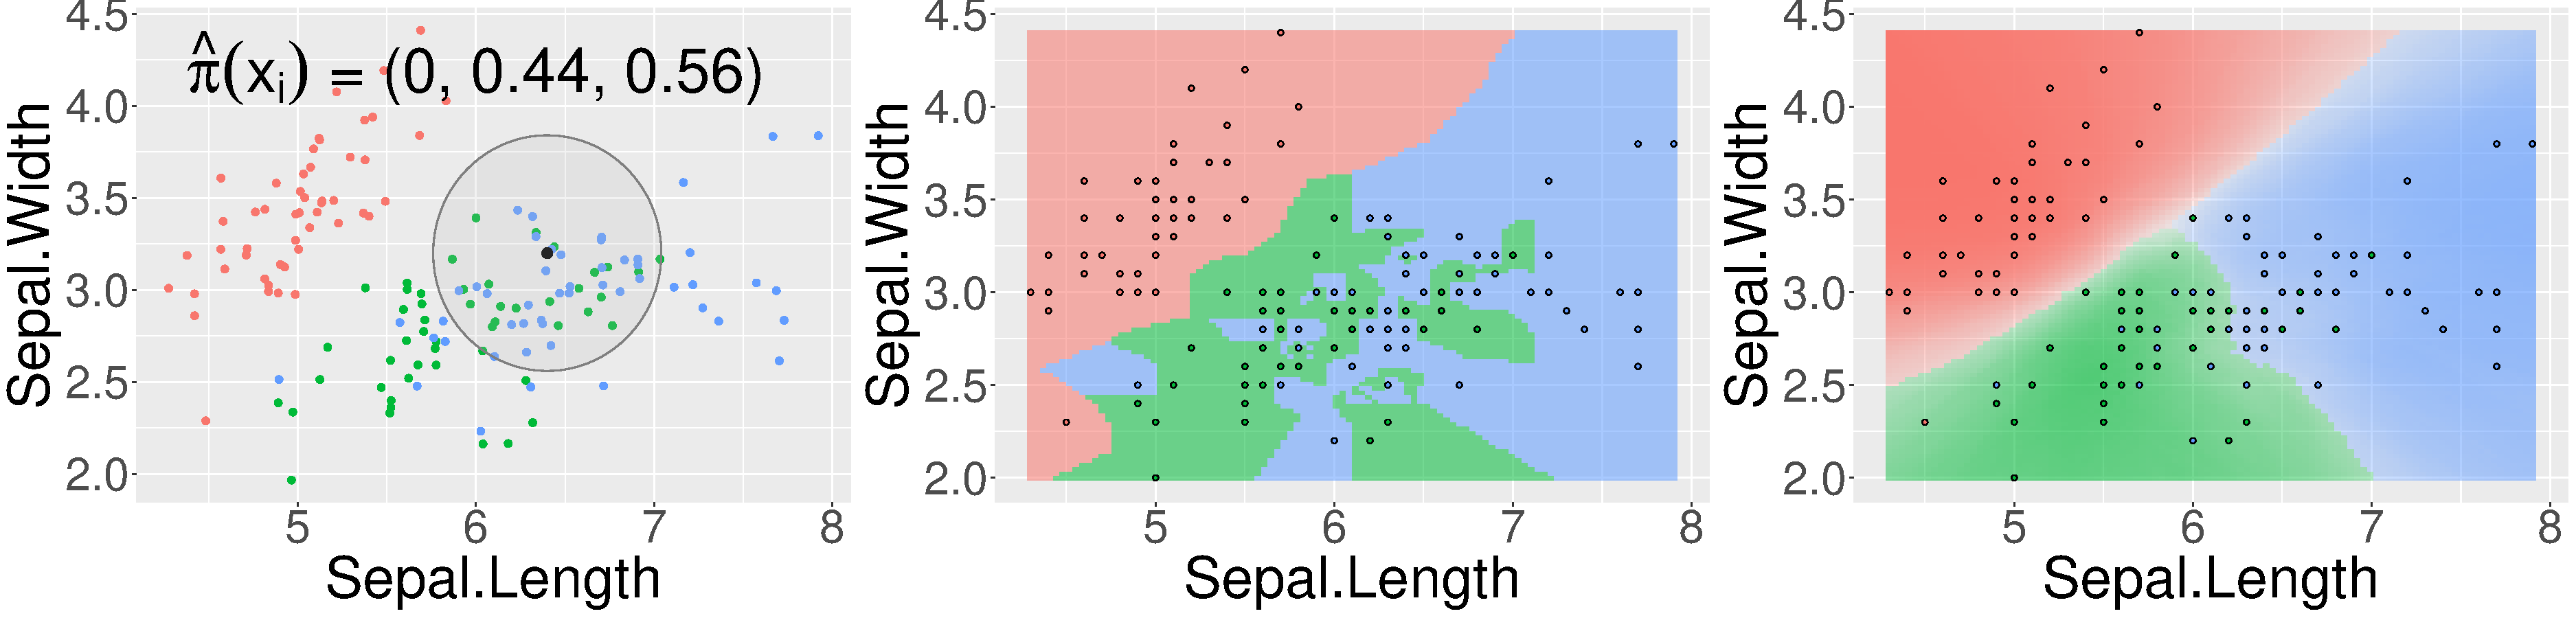
\includegraphics[width=\textwidth]{figure/knn-neighborhood.pdf}
  \end{minipage}%
  \hfill
  \begin{minipage}{0.25\textwidth}
    \tiny
    \raggedright
    \textbf{Classification} \\
    \textit{Left}: Neighborhood for exemplary observation in \texttt{iris}, 
    $k = 50$ \\
    \textit{Middle}: Prediction surface for $k = 1$\\
    \textit{Right}: Prediction surface for $k = 50$
  \end{minipage}

  \begin{minipage}{0.7\textwidth}
  \, \, \, 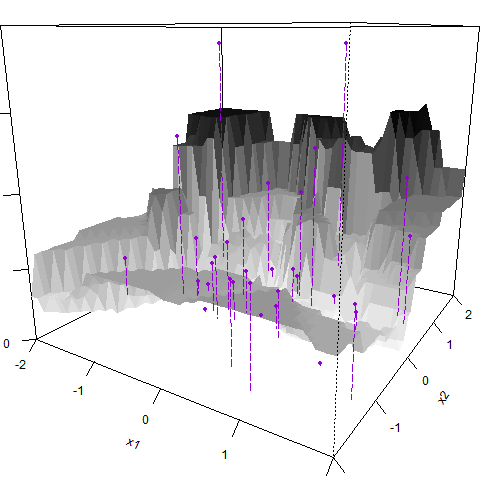
\includegraphics[width=0.25\textwidth]{figure/knn-reg-3d-3.png} \, \,
  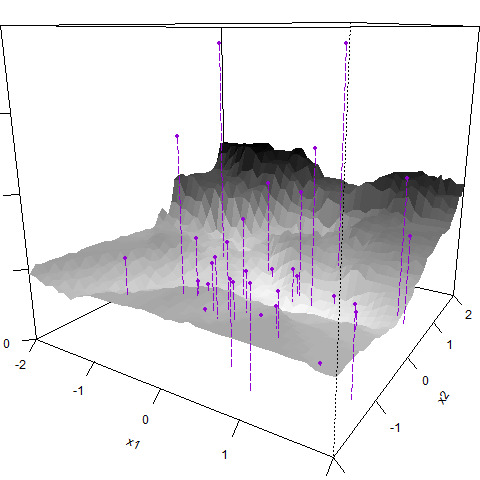
\includegraphics[width=0.25\textwidth]{figure/knn-reg-3d-7.png} \, \,
  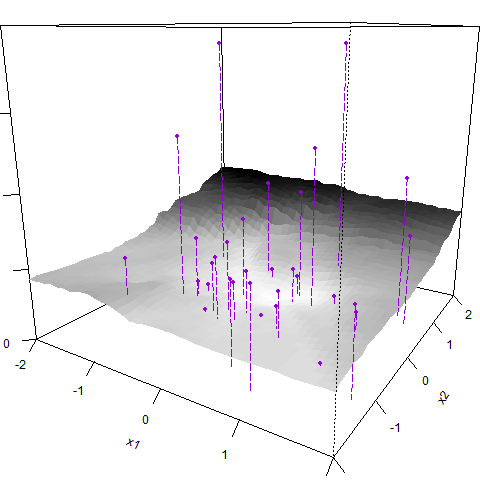
\includegraphics[width=0.25\textwidth]{figure/knn-reg-3d-15.png}
  \end{minipage}%
  \hfill
  \begin{minipage}{0.25\textwidth}
    \tiny
    \raggedright
    \textbf{Regression} \\
    \textit{Left}: Prediction surface for $k = 3$\\ 
    \textit{Middle}: Prediction surface for $k = 7$\\
    \textit{Right}: Prediction surface for $k = 15$
  \end{minipage}

  \medskip

  \begin{itemize}
      \item Small $k$ $\Rightarrow$ very local, "wiggly" decision boundaries
      \item Large $k$ $\Rightarrow$ rather global, smooth decision boundaries
  \end{itemize}

\end{frame2}



\begin{frame2}{$k$-NN -- method summary}

\highlight{Popular distance metrics}

\begin{itemize}
  \item Numerical feature space: Typically, \textbf{Minkowski} distances\\
  \splitVCC[0.6]{
    $d(\xv, \xtil) = \|\xv - \xtil \|_q = 
  \left( \sum_j | x_j - \tilde{x_j} |^q
  \right)^{\tfrac{1}{q}}$
    \begin{itemize}
    \item $q = 1$: \textbf{Manhattan} distance $\rightarrow d(\xv, \xtil) =
      \sum_j | x_j - \tilde{x_j} |$
    \item $q = 2$: \textbf{Euclidean} distance $\rightarrow d(\xv, \xtil) =
    \sqrt{\sum_j (x_j - \tilde{x_j})^2}$
    \end{itemize}
  }{
    \begin{center}
      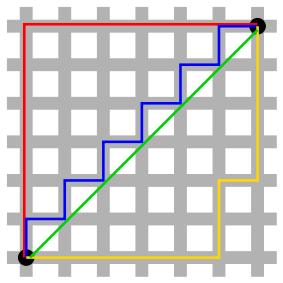
\includegraphics[width=.5\textwidth]{figure/manhattan_distance.png} %https://es.m.wikipedia.org/wiki/Archivo:Manhattan_distance.svg
     \end{center}
     Manhattan vs. Euclidean (green) \\
     {\tiny \href{https://es.m.wikipedia.org/wiki/Archivo:Manhattan_distance.svg}{https://es.m.wikipedia.org/wiki/Archivo:Manhattan\_distance.svg}}
  }

  \item Mixed feature space: 
  \begin{itemize}
%      \item Minkowski distances not applicable anymore
      \item \textbf{Gower distance} for numerical, categorical and missing data:\\ % (defined as \textit{similarity} by Gower, 1971):\\ %https://www.jstor.org/stable/2528823?seq=3#metadata_info_tab_contents
            - numerical: $d(x_i,x_j) =  \dfrac{|x_i-x_j|}{\max(x)-\min(x)}$\\
            - categorical: $d(x_i,x_j) =
            \begin{cases}
              1, \text{if\,} x_i \neq x_j\\
              0, \text{if\,} x_i = x_j
            \end{cases}$\\
            - Gower distance as average over individual scores
  \end{itemize}
  %\item \textbf{Custom} distance measures applicable
  \item Optional \textbf{weighting} for beliefs about varying feature
  importance
\end{itemize}
\vfill
  

\end{frame2}

\begin{frame2}{$k$-NN -- Implementation \& Practical hints}
  \footnotesize

\highlight{Preprocessing} ~~
Features should be standardized or normalized

\medskip

\highlight{Implementation}
\begin{itemize}
  \item \textbf{R:} \texttt{mlr3} learners (calling \texttt{kknn::kknn()})
  \begin{itemize}
    \item \textbf{Classification:}\\ 
    - \texttt{LearnerClassifKKNN}\\
    - \texttt{fnn::knn()}
    \item \textbf{Regression:}\\
    - \texttt{LearnerRegrKKNN}\\
    - \texttt{fnn::knn.reg()}
    \item Nearest Neighbour Search in $\order(N \log N)$: \texttt{RANN::nn2()}
  \end{itemize}
\end{itemize}
\end{frame2}



\begin{frame2}{$k$-NN -- Implementation \& Practical hints}
\begin{itemize}
  \item \textbf{Python:} From package \texttt{sklearn.neighbors} 
  \begin{itemize}
    \item \textbf{Classification:}\\ 
    - \texttt{KNeighborsClassifier()}\\
    - \texttt{RadiusNeighborsClassifier()} as alternative if data not uniformly sampled
    \item \textbf{Regression:}\\
    - \texttt{KNeighborsRegressor()} \\
    - \texttt{RadiusNeighborsRegressor()} as alternative if data not uniformly sampled
  \end{itemize}
\end{itemize}
  
\end{frame2}

\begin{frame2}{$k$-NN -- Pros \& Cons}
  \footnotesize

\begin{columns}[onlytextwidth]
  \begin{column}{0.5\textwidth}
    \highlight{Advantages}
    \footnotesize
    \begin{itemize}
      \positem Algorithm \textbf{easy} to explain and implement
      % \positem Applicable to both regression and classification
      \positem No distributional or functional \textbf{assumptions}\\
      $\rightarrow$ able to model data of \textbf{arbitrary complexity} %(in theory) 
      \positem No \textbf{training} or \textbf{optimization} required 
      %\positem Constant evolvement with \textbf{new data}
      \positem \textbf{local model} $\rightarrow$ \textbf{nonlinear} decision boundaries
      \positem Easy to \textbf{tune} (few hyperparameters)\\
      $\rightarrow$ number of neighbors $k$, distance metric
      % \positem Only one \textbf{hyperparameter} to tune
      \positem \textbf{Custom} distance metrics can often be easily designed to incorporate domain knowledge
    \end{itemize}
  \end{column}
  \begin{column}{0.5\textwidth}
    \highlight{Disadvantages}
    \footnotesize
    \begin{itemize}
      \negitem Sensitivity w.r.t. \textbf{noisy} or \textbf{irrelevant} features and outliers due to dependency on distance measure
      \negitem Heavily affected by \textbf{curse of dimensionality}
      \negitem Bad performance when feature \textbf{scales} are not consistent with feature relevance
      \negitem Poor handling of data \textbf{imbalances} (worse for more global model, i.e., large $k$)
      %\negitem High \textbf{memory} consumption of distance computation
    \end{itemize}
  \end{column}
\end{columns}
  
\end{frame2}

\begin{frame2}{Generalized Linear Models -- method summary}
  \maketag{regression} \maketag{classification} \maketag{PARAMETRIC} 
\maketag{WHITE-BOX} \maketag[50]{Feature selection}

\highlight{General idea} ~~ Represent target as function of linear predictor
$\thx$ (weighted sum of features)\\
$\rightarrow$ \textbf{Interpretation:} if feature $x_j$ increases by 1 unit, the linear predictor changes by $\theta_j$ units

\highlight{Hypothesis space} ~~
$\Hspace = \left\{f: \Xspace \to \R ~|~\fx = \phi(\thetav^\top \xv)\right\}$, 
with suitable transformation $\phi(\cdot)$, e.g.,

\begin{itemize}
  \item \textbf{Linear Regression}: $\Yspace = \R$, $\phi$ identity
  % $\rightarrow$ continous output
  \item \textbf{Logistic Regression}: $\Yspace = \{0, 1\}$, logistic sigmoid $\phi(\thx) = \frac{1}{1 + \exp(- \thx)} 
  =: \pixt$\\
  $\Rightarrow$ Decision rule: Linear hyperplane
\end{itemize}
\end{frame2}

\begin{frame2}{Generalized Linear Models -- method summary}
\highlight{Loss functions}

\twobytwo{
  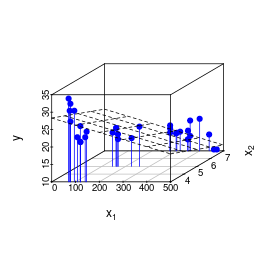
\includegraphics[width=0.7\textwidth, trim=0 40 0 0, clip]{
    figure/lm_3d.png} \\
    \tiny{Linear regression hyperplane}
}{
  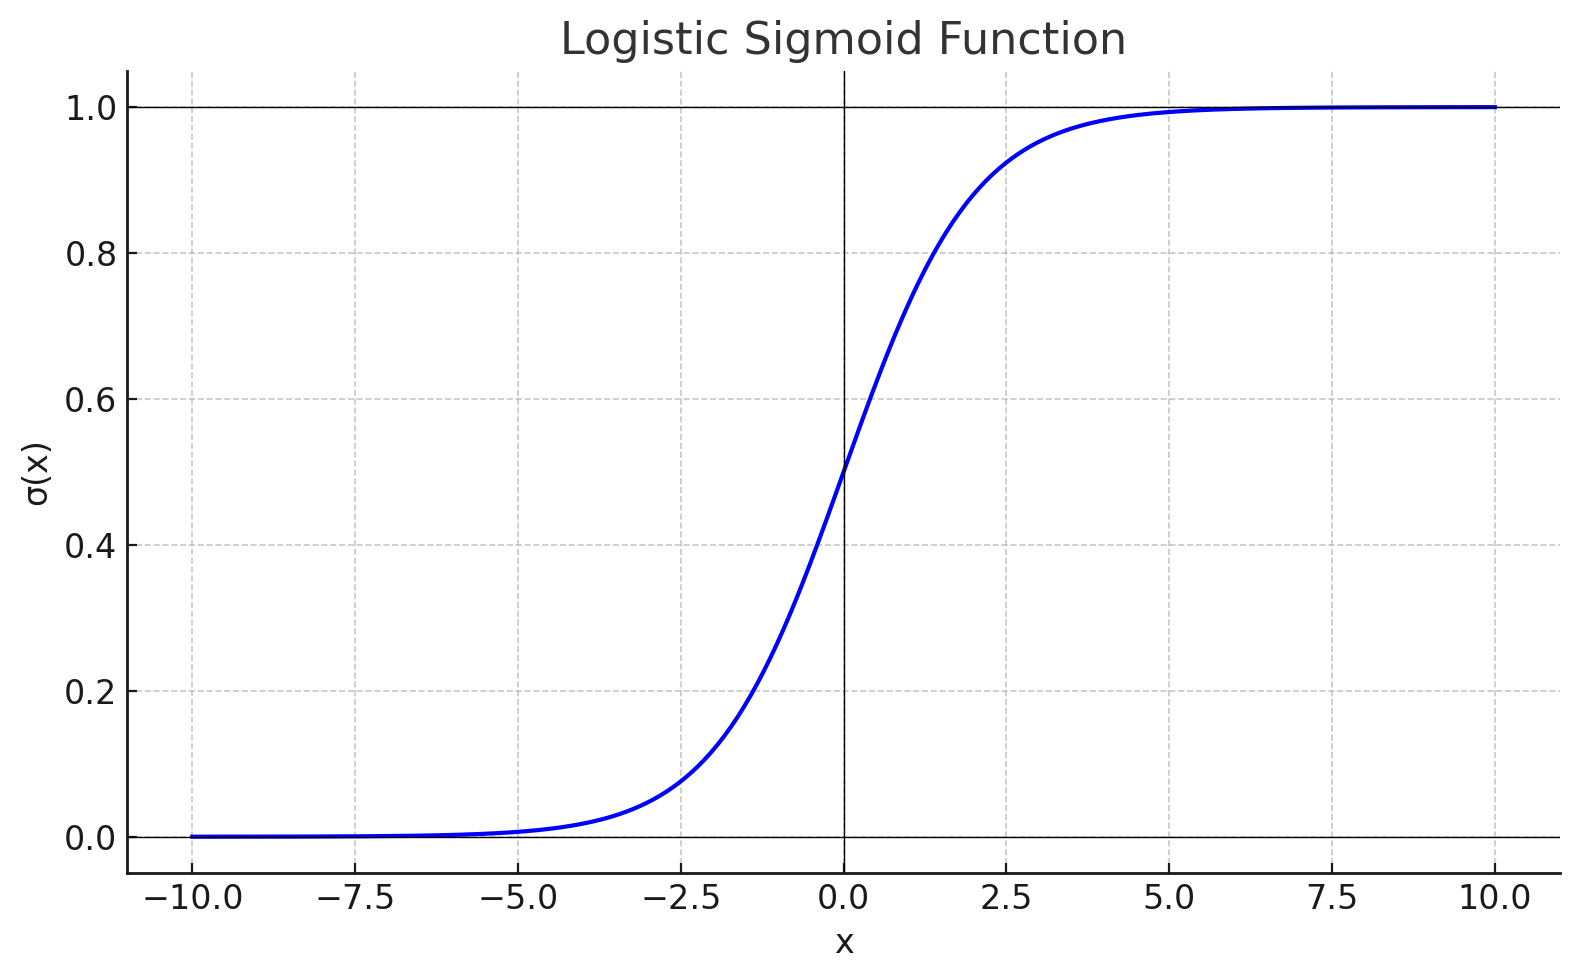
\includegraphics[width=0.7\textwidth, trim=0 40 0 0, clip]{../supervised-classification/figure/reg_class_loss_1.png}\\
    \tiny{Logistic sigmoid function}
}{
  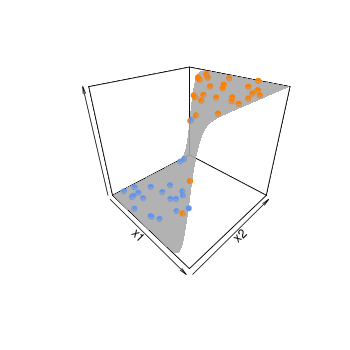
\includegraphics[width=0.7\textwidth, trim=30 50 0 0, clip]{
    figure/logreg_3d}\\
    \tiny{Logistic function for bivariate input and loss-minimal $\thetav$}
}{
  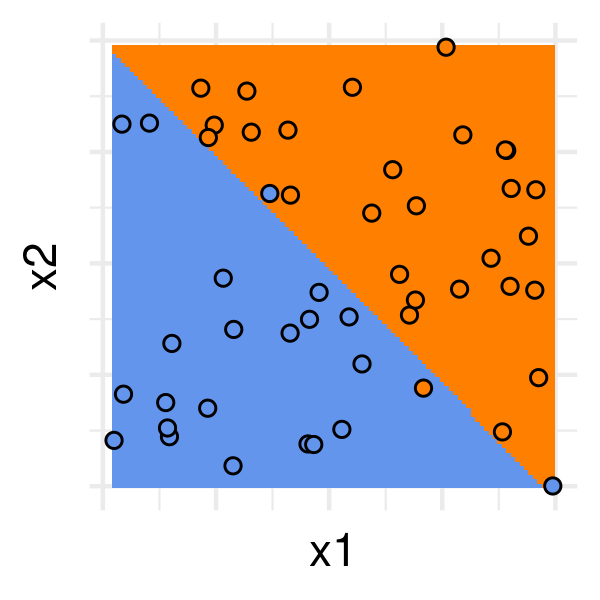
\includegraphics[width=0.7\textwidth]{figure/logreg_2d}\\
    \tiny{Corresponding separating hyperplane}
}
\end{frame2}

\begin{frame2}{Generalized Linear Models -- method summary}
\begin{itemize}
  \item \textbf{Lin. Regr.}:
  \begin{itemize}
    
    \item Typically, based on \textbf{quadratic} loss (OLS estimation): 
    $$L\left(y, f\right) = \left(y - f \right)^2$$ %~~
    %$\Rightarrow$ OLS estimation
    % \item Alternatives: e.g., \textbf{absolute} or \textbf{Huber} loss (both 
    % improving robustness)
  \end{itemize}
  \item \textbf{Log. Regr.}: Based on \textbf{bernoulli / log / cross-entropy} loss ~ 
  %$\Rightarrow \risket = \sumin -\yi \log \left(\pixii\right) - (1 - \yi) \log \left(1 - \pixii \right)$
  \begin{itemize}
      \item Loss based on scores
      \begin{eqnarray*}
    L\left(y, f\right) &=& \ln\left(1+\exp\left(-y \cdot f\right)\right) \quad \text{for } y \in \setmp\\
    L\left(y, f\right) &=& - y \cdot f + \log\left(1 + \exp\left(f\right)\right) \quad \text{for } y \in \setzo 
    \end{eqnarray*}
    \item Loss based on probabilities:
      \begin{eqnarray*}
    L\left(y, \pi\right) &=& \ln\left(1+\exp\left(-y \cdot \log \left(\pi\right)\right)\right) \quad \text{for } y \in \setmp\\
    L\left(y, \pi\right) &=& -y \log \left(\pi\right) - (1 - y) \log \left(1 - \pi \right)  \quad \text{for } y \in \setzo 
    \end{eqnarray*}
  \end{itemize}
\end{itemize}
\end{frame2}

\begin{frame2}{Generalized Linear Models -- method summary}

\highlight{Optimization} 

\begin{itemize}
    \item Minimization of the empirical risk
    \item For \textbf{OLS}: analytical solution $\thetavh = \olsest$
    \item For other loss functions: 
    \begin{itemize}
        \item \textbf{Log. Regr.}: Convex problem, solvable via second-order optimization methods (e.g. BFGS)
        \item \textbf{Else}: Numerical optimization 
    \end{itemize}
    
\end{itemize}

\medskip

% \highlight{Hyperparameters} ~~ None

%\medskip

\highlight{Multi-class extension of logistic regression}

\begin{itemize}
  \item Estimate \textbf{class-wise} scoring functions:
  $\Rightarrow \pi: \Xspace \rightarrow \unitint^g, ~
  \pix = (\pikx[1], \dots, \pikx[g]), ~\sumkg \pikx = 1$
  \item Achieved through \textbf{softmax} transformation: 
  $\pikxt = \exp(\thetav_k^\top \xv) \big/ \sum_{j=1}^g \exp(\thetav_j^\top 
  \xv)  $
  \item Multi-class log-loss: $\Lpixy = - \sumkg \I_{\{y = k\}} \log(\pikx)$
  \item Predict class with maximum score (or use thresholding variant)
\end{itemize}

% \highlight{Runtime behavior} ~~ $\mathcal{O}(p^2 \cdot n + p^3)$ for $n$ 
% observations and $p$ features
\end{frame2}


\begin{frame2}{Generalized Linear Models -- regularization}

  \highlight{General idea}

\begin{itemize}
  \item Unregularized LM: risk of \textbf{overfitting} in high-dimensional 
  space with only few observations
  %\item \textbf{Goal}: find compromise between model fit and generalization by adding \textbf{penalty term}
  \item \textbf{Goal}: avoidance of overfitting by adding \textbf{penalty term}
%  \item Regularization ubiquitous in ML, with similar techniques
\end{itemize}

%\medskip

% \highlight{Hypothesis space} ~~\\
% $\Hspace = \left\{f: \Xspace \to \R ~|~\fx = \phi(\thetav^\top \xv)\right\}$, 
% where $\phi(\cdot)$ is a transformation function.


%$\Hspace = \{ \theta_0 + \thx\ |\ (\theta_0, \thetav) \in \R^{p+1} \} $

        
\highlight{Regularized empirical risk}

\begin{itemize}
  \item Empirical risk function \textbf{plus complexity penalty} 
  $J(\thetav)$, controlled by shrinkage parameter $\lambda > 0$:
  $\riskrt := \risket + \lambda \cdot J(\thetav)$
  %\item Popular regularizers
  %\begin{itemize} 
    \item \textbf{Ridge} regression: L2 penalty $J(\thetav) = \|\thetav\|_2^2 $
    \item \textbf{LASSO} regression: L1 penalty $J(\thetav) = \|\thetav\|_1 $
  %\end{itemize}

\end{itemize}

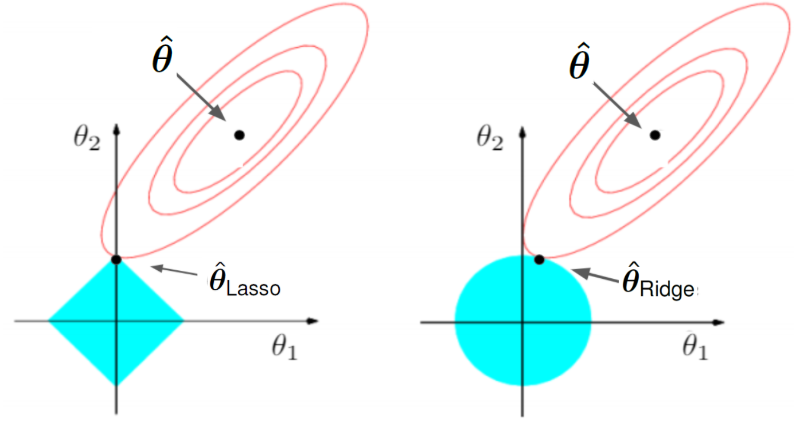
\includegraphics[width=0.5\textwidth]{figure/l1_l2_hat.png}

\end{frame2}

\begin{frame2}{Generalized Linear Models -- regularization}

\highlight{Optimization under regularization}
\begin{itemize}
  \item \textbf{Ridge}: analytically with 
  $\thetavh_{\text{Ridge}} = (\Xmat^\top \Xmat  + \lambda \id)^{-1} \Xmat^\top 
  \yv$
  \item \textbf{LASSO}: numerically with, e.g., (sub-)gradient descent
\end{itemize}

\highlight{Choice of regularization parameter}

\begin{itemize}
  \item Standard hyperparameter optimization problem
  \item E.g., choose $\lambda$ with minimum mean cross-validated error 
  %(default in R package \texttt{glmnet})
\end{itemize}


\highlight{Ridge vs. LASSO} 

\begin{itemize}
  \item \textbf{Ridge}
  \begin{itemize} 
    \item Global shrinkage $\Rightarrow$ overall smaller but still dense $\thetav$
    \item Applicable with large number of influential features,
    correlated variables' coefficients are shrinked by equal amount
  \end{itemize}
  \item \textbf{LASSO}
  \begin{itemize} 
    \item Actual variable selection by shrinking coefficients to zero
    \item Suitable for sparse problems, ineffective with correlated 
    features (randomly selecting one)
  \end{itemize}  
\end{itemize}

\end{frame2}


\begin{frame2}{Generalized Linear Models -- regularization}


\begin{columns}[T, totalwidth=\textwidth]
  \begin{column}{0.62\textwidth}

  \begin{itemize}
    \item Neither overall better $\Rightarrow$ \textbf{elastic net}
    \item Weighted combination of Ridge and LASSO
    \item Introducing additional penalization coefficient: %$\riskrt = \risket + \lambda_1 \cdot \|\thetav\|_1 + \lambda_2 \cdot \|\thetav\|_2^2$\\
    $\riskrt = \risket 
    + \lambda \cdot P_{\alpha}(\thetav)$, with\\
    $P_{\alpha}(\thetav) = [\alpha \cdot \|\thetav\|_1 + (1 - \alpha) \cdot \frac{1}{2} \cdot \|\thetav\|_2^2]$
  \end{itemize}  


\end{column}

\begin{column}{0.38\textwidth}
\tiny
\centering
\begin{columns}[T, totalwidth=\textwidth]
\begin{column}{0.5\textwidth}
\tiny
\begin{center}
\textbf{Ridge} performs better for correlated features: \\ 
\medskip
$\boldsymbol{\beta}=(\underbrace{2,\ldots,2}_{5},\underbrace{0,\ldots,0}_{5})$\\
$ \operatorname{cor}(\Xmat_{i},\Xmat_{j})=0.8^{|i-j|}, \forall i, j$
  \end{center}
\end{column}
\begin{column}{0.5\textwidth} \tiny

\begin{center}
\textbf{Lasso} performs better for uncorrelated features: \\
\medskip
$\boldsymbol{\beta}=(2, 2, 2,\underbrace{0,\ldots,0}_{7})$ \\
$\operatorname{cor}(\Xmat_{i},\Xmat_{j})= 0, \forall i \neq j$
\end{center}
\end{column}
\end{columns}



          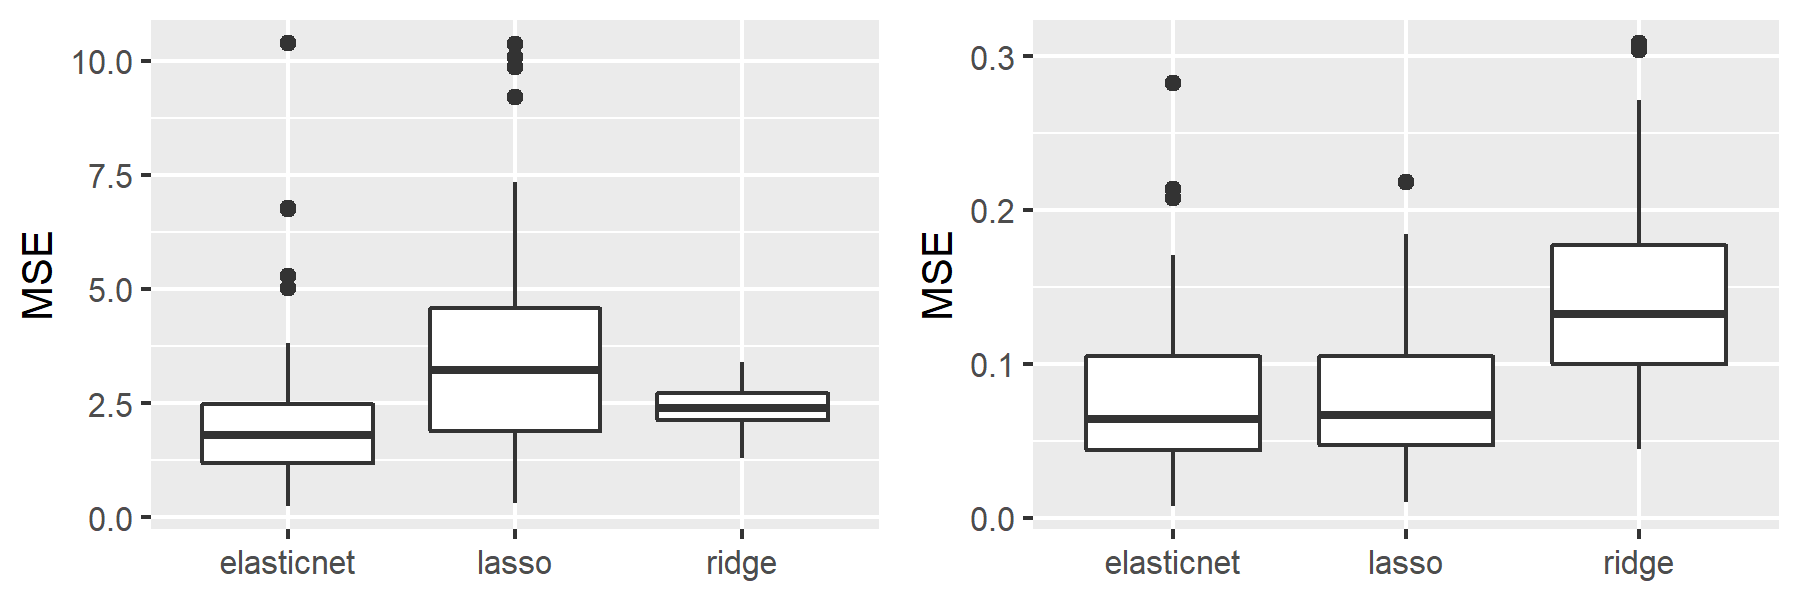
\includegraphics[width=\textwidth]{figure/enet_lasso_ridge_mse.png}
          
          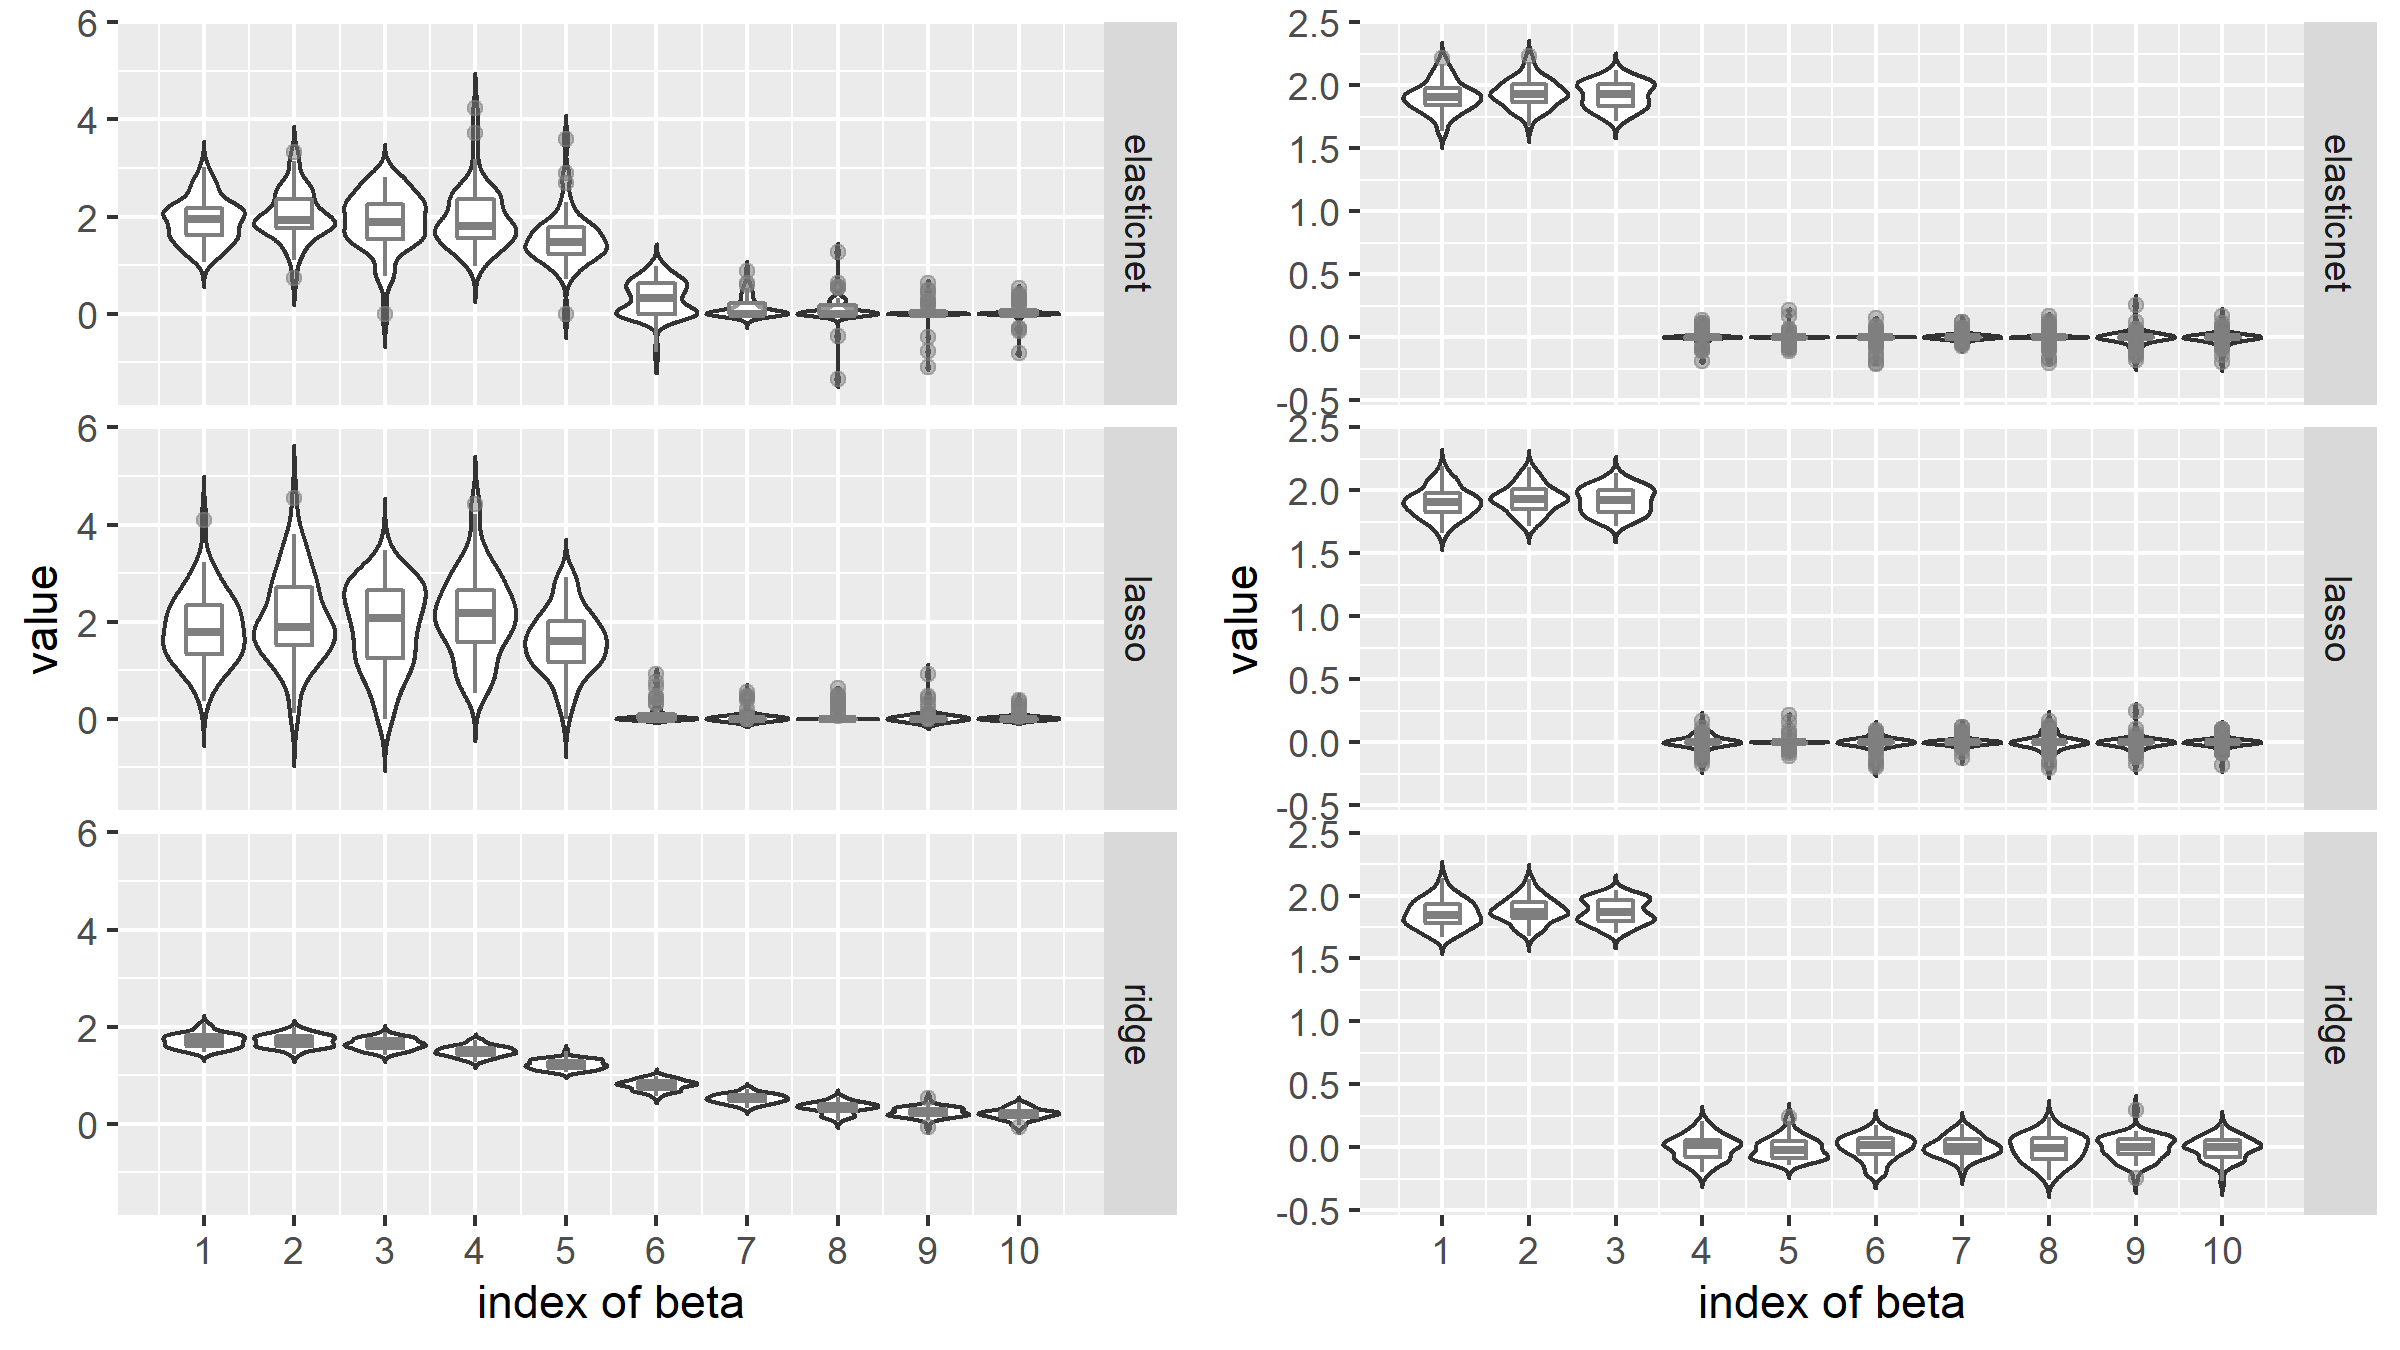
\includegraphics[width=\textwidth]{figure/enet_tradeoff.png}
\end{column}

\end{columns}
  
\end{frame2}


\begin{frame2}{Generalized Linear Models -- Implementation}
  \highlight{Implementation}

\begin{itemize}
  \item \textbf{R:}
  \begin{itemize}
    \item \textbf{Unregularized:} \texttt{mlr3} learner \texttt{LearnerRegrLM}, 
    calling \texttt{stats::lm()} / \texttt{mlr3} learner 
    \texttt{LearnerClassifLogReg}, calling \texttt{stats::glm()}
    \item \textbf{Regularized / ElasticNet:} \texttt{mlr3} learners 
    \texttt{LearnerClassifGlmnet} / 
    \texttt{LearnerRegrGlmnet}, calling \texttt{glmnet::glmnet()}
    \item For \textbf{large classification} data: \texttt{mlr3} learner     
    \texttt{LearnerClassifLiblineaR}, calling \texttt{LiblineaR::LiblineaR()} uses fast coordinate descent
  \end{itemize}
\end{itemize}
\end{frame2}

\begin{frame2}{Generalized Linear Models -- Implementation}
\begin{itemize}
  \item \textbf{Python:} From package \texttt{sklearn.linear\_model} 
  \begin{itemize}
    \item \textbf{Unregularized:}\\ 
    - \texttt{LinearRegression()}\\
    - \texttt{LogisticRegression(penalty = None)}
    \item \textbf{Regularized:}\\
    - \textit{Linear regression:} \texttt{Lasso(),Ridge(),ElasticNet()} \\
    - \textit{Logistic regression:} \texttt{LogisticRegression(penalty = \{‘l1’, ‘l2’, ‘elasticnet’\})}
    \item Package for advanced \textbf{statistical} models: \texttt{statsmodels.api} 
  \end{itemize}
\end{itemize}

%% WOULD DELTETE THIS!
%  \highlight{\textcolor{blue}{Check assumptions??} }\\
% Linear models are effective if the following assumptions are fulfilled:
%  \begin{itemize}
%   \item \textbf{linearity}: The expected response is a linear combination of the features.
%   \item \textbf{homoscedasticity}: The variance of residuals is equal for all features.
%   \item \textbf{independence}: All observations are independent of each other.
%   \item \textbf{normality}: Y is normally distributed for any fixed value of the features
% \end{itemize}
  
\end{frame2}

\begin{frame2}{Generalized Linear Models -- Pros \& Cons}

  \begin{columns}[onlytextwidth]
    \begin{column}{0.5\textwidth}
      \highlight{Advantages}
      
      \begin{procon}
        \setlength{\itemsep}{1pt}
        \setlength{\parskip}{1pt}
        \positem \textbf{Simple and fast} implementation
        \positem \textbf{Analytical} solution for L2 loss
        %\positem \textbf{Cheap} computation
        \positem Applicable for any \textbf{dataset size}, as long as number of 
        observations $\gg$ number of features
        \positem Flexibility \textbf{beyond linearity} with polynomials, 
        trigonometric transformations, interaction terms etc.
        \positem Intuitive \textbf{interpretability} via feature effects
        % \item fits \textbf{linearly} separable data sets very well
        \positem Statistical hypothesis \textbf{tests} for effects available
      \end{procon}
    \end{column}
  
    \begin{column}{0.5\textwidth}
      \highlight{Disadvantages}
      
      \begin{itemize}
        \negitem \textbf{Nonlinearity} of many real-world problems
        \negitem Further restrictive \textbf{assumptions}: linearly independent 
        features, homoskedastic residuals, normality of conditional response 
        %\textcolor{blue}{actually relevant in ML?}
        \negitem \textbf{Sensitivity}: outliers, noise
        \negitem LM can \textbf{overfit} (e.g., many features and few observations) 
        \negitem Feature \textbf{interactions} must be handcrafted\\
        $\rightarrow$ practically infeasible for higher orders
        %\negitem No handling of \textbf{missing} data
      \end{itemize}
    \end{column}
  \end{columns}
  
\end{frame2}


\begin{frame2}{Generalized Additive Models -- method summary}
  % \maketag{SUPERVISED} 
\maketag{regression} \maketag{classification} \maketag[50]{(NON)PARAMETRIC}
\maketag[50]{WHITE-BOX} \maketag[50]{Feature selection}

\highlight{General idea}
\begin{itemize}
  \item Same as GLM, but introduce \textbf{flexibility} through
  \textbf{nonlinear (smooth)} effects $f_j(x_j)$
  \item Typically, combination of linear \& smooth effects
  \item Smooth effects also conceivable for feature interactions
\end{itemize}

\highlight{Hypothesis space} ~~
$\Hspace = \left\{f: \Xspace \to \R ~|~\fx = \phi \left(\theta_0 + \textstyle \sumjp
f_j(x_j) \right) \right\}$,
suitable transformation $\phi(\cdot)$, intercept $\theta_0$, smooth
functions $f_j(\cdot)$

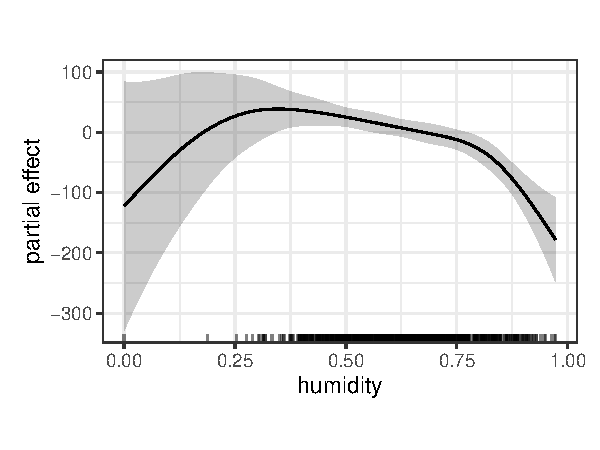
\includegraphics[width=0.28\textwidth]{figure/gam_bike_partial_effect}
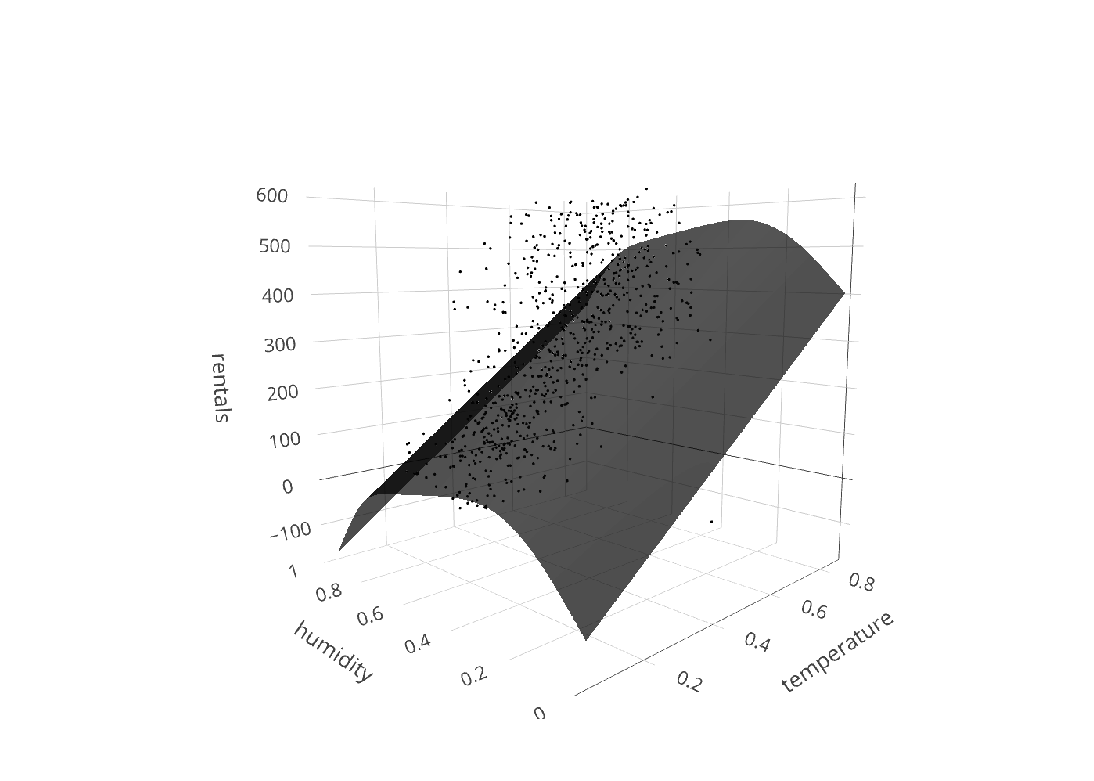
\includegraphics[width=0.35\textwidth, trim=0 0 0 80, clip]{figure/gam_bike_pred}

\tiny
Prediction of \texttt{bike rentals} from smooth term of \texttt{humidity}
(left: partial effect) and linear term of \texttt{temperature} (right: bivariate
prediction).
\normalsize

\end{frame2}


\begin{frame2}{Generalized Additive Models -- method summary}

\highlight{Smooth functions}

\begin{itemize}
  \item Non-/semi-/parametric approaches conceivable
  \item Frequently: express $f_j$ as weighted sum of \textbf{basis functions}
  $\rightsquigarrow$ model \textbf{linear} in weight coefficients again
  \begin{itemize}
      \item Use fixed basis of functions $b_1, \dots, b_K$ and estimate
      associated coefficients $\gamma_1, \dots, \gamma_K$ \\ $\rightsquigarrow$
      $f_j(x_j) = \textstyle \sum_{k=1}^{K_j} \gamma_{j, k} b_k(x_j)$
      \item Popular types of basis functions
      \begin{itemize}
        \footnotesize
        \item Polynomial $\rightsquigarrow$ smoothing/TP-/B-\textbf{splines}
        \item Radial $\rightsquigarrow$ \textbf{Kriging}
        \item Trigonometric $\rightsquigarrow$ \textbf{Fourier/wavelet} forms
      \end{itemize}
    \end{itemize}
    \item Alternatives: \textbf{local regression (LOESS)},
    kernel-smoothing, \dots
\end{itemize}

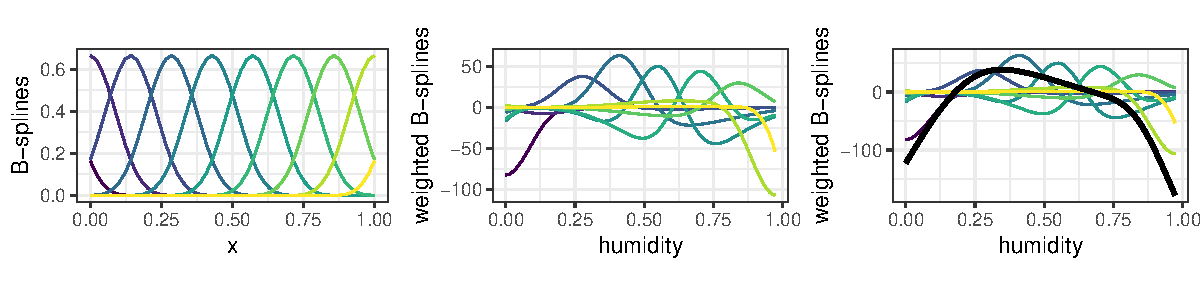
\includegraphics[width=0.7\textwidth]{figure/gam_bike_spline_basis}

\tiny
Left: B-spline basis with 9 basis functions.
Middle: BFs weighted with coefficients estimated for
\texttt{humidity}.
Right: sum of weighted BFs in black (= partial effect).

\end{frame2}

\begin{frame2}{Generalized Additive Models -- method summary}
\highlight{Regularization}
\begin{itemize}
    \item Smooth functions possibly very flexible $\rightsquigarrow$
    regularization vital to prevent overfitting
    \item Control \textbf{smoothness}
    \begin{itemize}
      \item \textbf{Basis-function approaches}: control number; impose penalty
      on coefficients
      (e.g., magnitude or differences between coefficients of neighboring
      components) \& control associated hyperparameter
      \item \textbf{Local smoothers}: control width of smoothing window
      (larger $\rightsquigarrow$ smoother)
    \end{itemize}
\end{itemize}

\begin{minipage}{0.65\textwidth}
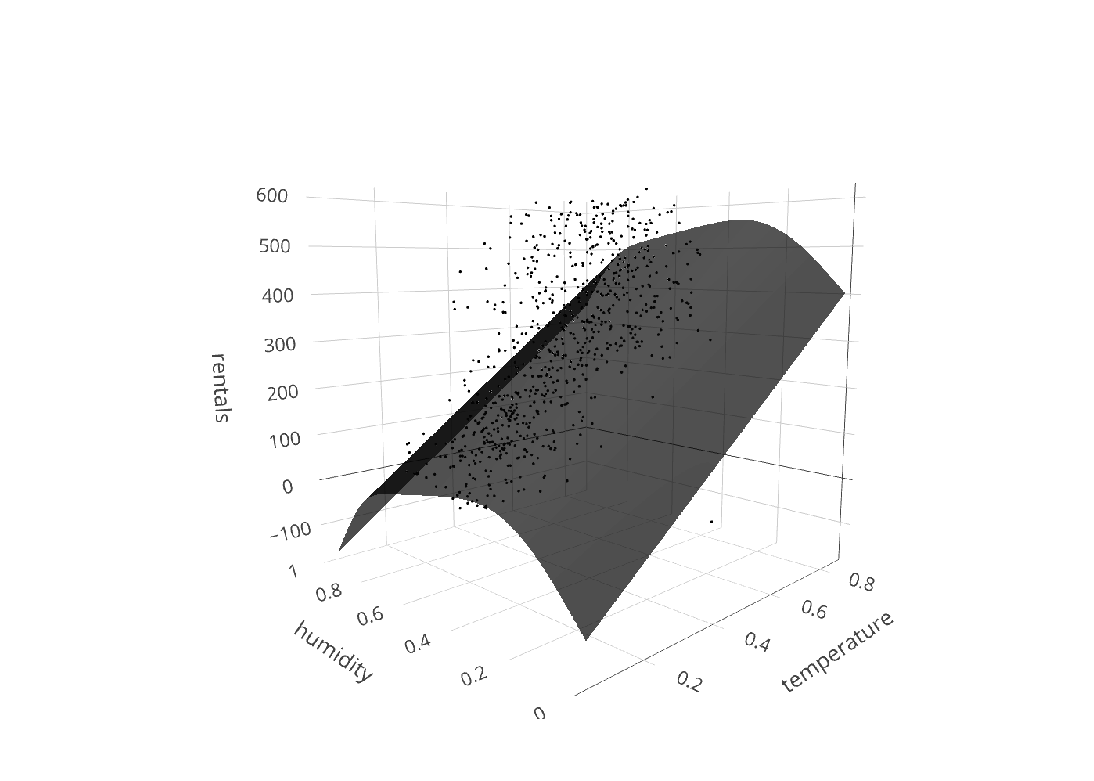
\includegraphics[width=0.45\textwidth, trim=0 0 80 80, clip]{
figure/gam_bike_pred}
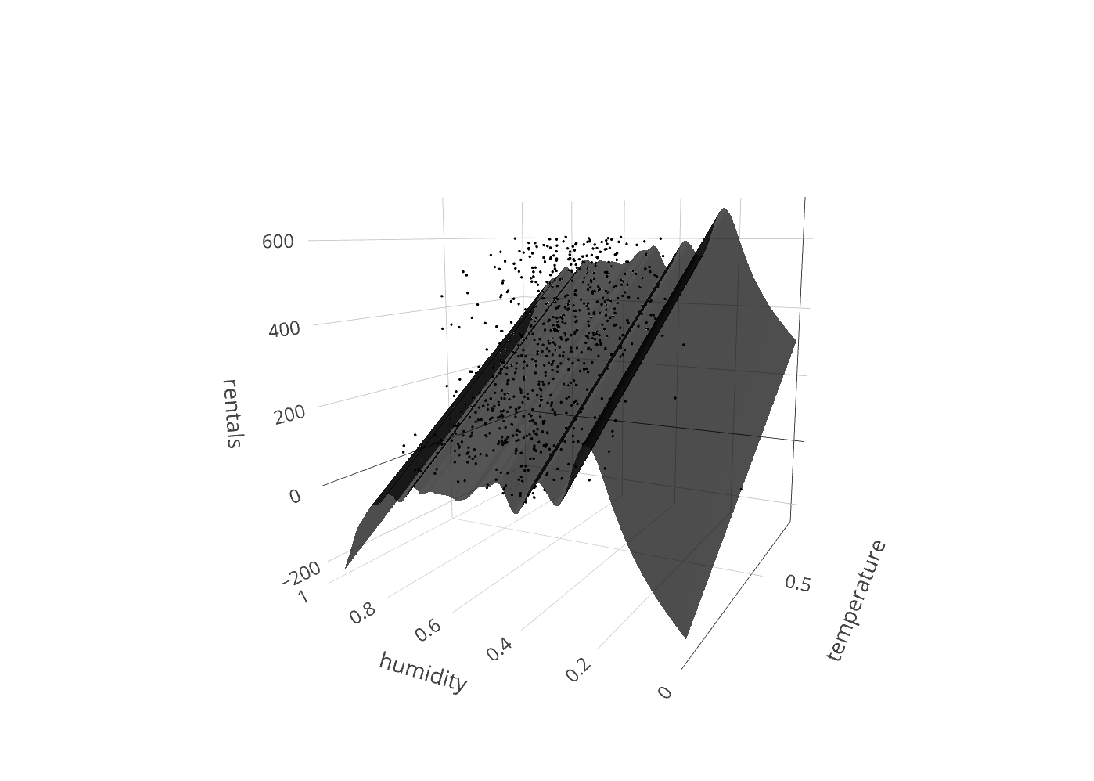
\includegraphics[width=0.45\textwidth, trim=80 0 0 80, clip]{
figure/gam_bike_pred_wiggly}
\hfill
\end{minipage}
\begin{minipage}{0.3\textwidth}
\tiny \raggedright
Prediction surfaces for \texttt{bike rentals} with 9 (left) and 500 (right)
basis functions in smooth \texttt{humidity} term.
Higher number of basis functions yields more local, less smooth model.
\end{minipage}

\end{frame2}

\begin{frame2}{Generalized Additive Models -- method summary}

\highlight{Loss functions} ~~ Same as in GLM $\rightsquigarrow$ essentially:
use \textbf{negative log-likelihood}

\highlight{Optimization}
\begin{itemize}
  \item \textbf{Coefficients} (of smooth + linear terms):
  penalized MLE, Bayesian inference
  \item \textbf{Smoothing hyperparameters}: typically, generalized
  cross-validation
\end{itemize}

\end{frame2}


\begin{frame2}{Generalized Additive Models -- implementation}

  \highlight{Implementation}

\begin{itemize}
  \item \textbf{R:} \texttt{mlr3} learner \texttt{LearnerRegrGam},
    calling \texttt{mgcv::gam()}
  \begin{itemize}
      \item Smooth terms: \texttt{s(\dots, bs="<basis>")} or \texttt{te(\dots)}
      for multivariate (tensorproduct) effects
      \item Link functions: \texttt{family=$\{$Gamma, Binomial, \dots $\}$}
  \end{itemize}
    \item \textbf{Python}: \texttt{GLMGam} from package \texttt{statsmodels};
    package \texttt{pygam}
\end{itemize}

\end{frame2}

\begin{frame2}{Generalized additive models -- Pros \& Cons}

\begin{columns}[onlytextwidth]
  \begin{column}{0.5\textwidth}
    \highlight{Advantages}

%    Strengths of GLMs, plus \dots
    \begin{itemize}
      \positem \textbf{Simple and fast}
%      \positem \textbf{Analytical} solution for L2 loss
      %\positem \textbf{Cheap} computation
      \positem Applicable for any \textbf{dataset size}, as long as number of
      observations $\gg$ number of features
      \positem High \textbf{flexibility} via smooth effects
      \positem Easy to \textbf{combine} linear \& nonlinear effects
      \positem Rather intuitive \textbf{interpretability} via feature effects
      % \item fits \textbf{linearly} separable data sets very well
      \positem Statistical hypothesis \textbf{tests} for effects available
    \end{itemize}
  \end{column}

  \begin{column}{0.5\textwidth}
    \highlight{Disadvantages}

%    Shortcomings of GLMs, plus \dots
    \begin{itemize}
      \negitem \textbf{Sensitivity} w.r.t. outliers and noisy data
      \negitem Feature \textbf{interactions} must be handcrafted\\
      $\rightarrow$ practically infeasible for higher orders
      \negitem Harder to \textbf{optimize} than GLM
      \negitem Additional \textbf{hyperparameters} (type of smooth functions,
      smoothness degree, \dots)
    \end{itemize}
  \end{column}
\end{columns}
  
\end{frame2}


\begin{frame2}{CART -- method summary}
  \footnotesize

% \maketag{Supervised} 
\maketag{regression} \maketag{classification}
\maketag{Nonparametric} \maketag{White-box} \maketag{Feature selection}

\splitVCC[0.6]{
  \highlight{General idea (CART -- Classification and Regression Trees)}
  \begin{itemize}
  \item Start at root node containing all data
  \item Perform repeated \textbf{axis-parallel binary splits} in feature space to obtain
  \textbf{rectangular partitions} at terminal nodes $Q_1, \dots, Q_M$
  \item Splits based on reduction of node \textbf{impurity} \\
  $\rightarrow$ empirical risk minimization (\textbf{ERM})
\end{itemize}
}{
  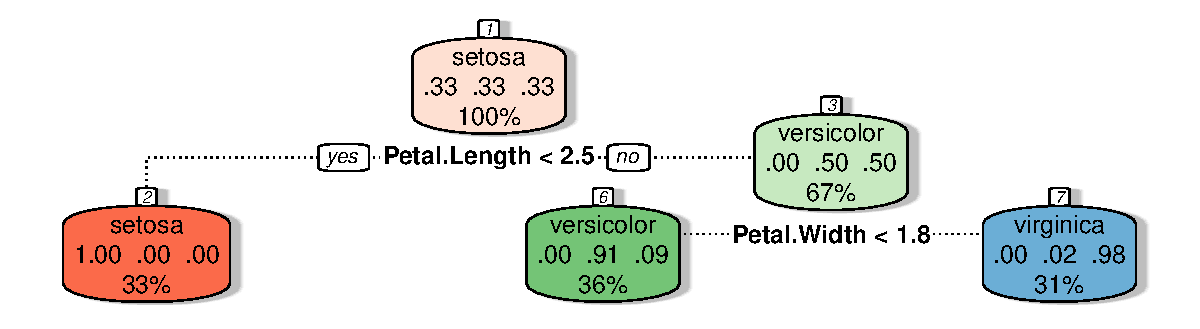
\includegraphics[width=\textwidth]{../cart/figure/cart_treegrow_22}
  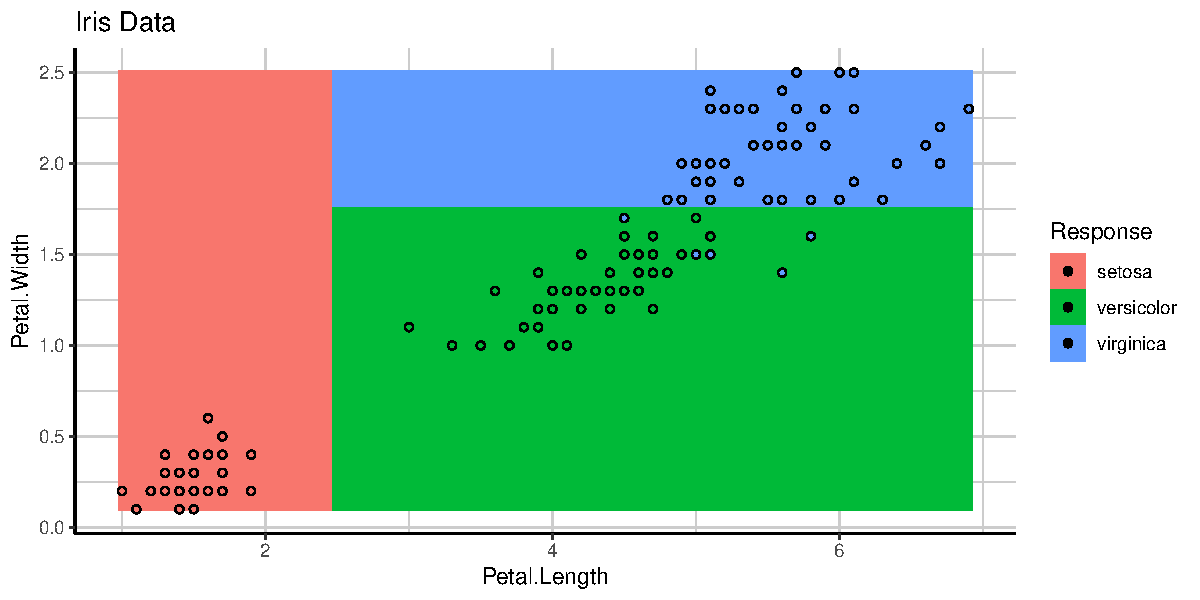
\includegraphics[width=\textwidth]{   ../cart/figure/cart_splitcriteria_1}
}



\begin{itemize}
  \item In each step:
  \begin{itemize}
    \item Find \textbf{optimal split} (feature-threshold combination) \\
    $\rightarrow$ greedy search
    \item Assign constant prediction $c_m$ to all obs. in $Q_m$\\
    $\rightarrow$ Regression: $c_m$ is average of $y$ \\
    $\rightarrow$ Classif.: $c_m$ is majority class (or class proportions)
    
  \item Stop when a pre-defined criterion is reached\\
  $\rightarrow$ See \highlight{Complexity control}
  \end{itemize}
\end{itemize}

\end{frame2}

\begin{frame2}{CART -- method summary}

%\medskip
    \highlight{Hypothesis space} ~~
$\Hspace = \left\{ \fx: \fx = \sum\limits_{m = 1}^M c_m \I(\xv \in Q_m) 
\right\}$

\footnotesize

\splitVCC[0.6]{
  \highlight{Empirical risk} \\
      \begin{itemize}
        \item Splitting \textbf{feature $x_j$ at split point $t$} divides a parent node $N_p$ into two child nodes:
      
          %\item Splitting \textbf{feature $x_j$ at split point $t$} divides a parent node $\Np$ into two child nodes:

                 $$ N_l = \{ (\xv, y) \in N_p: x_j \leq t \} \text{ and } N_r = \{ (\xv, y) \in N_p: x_j > t \} $$

      \end{itemize}
}{
  \centering 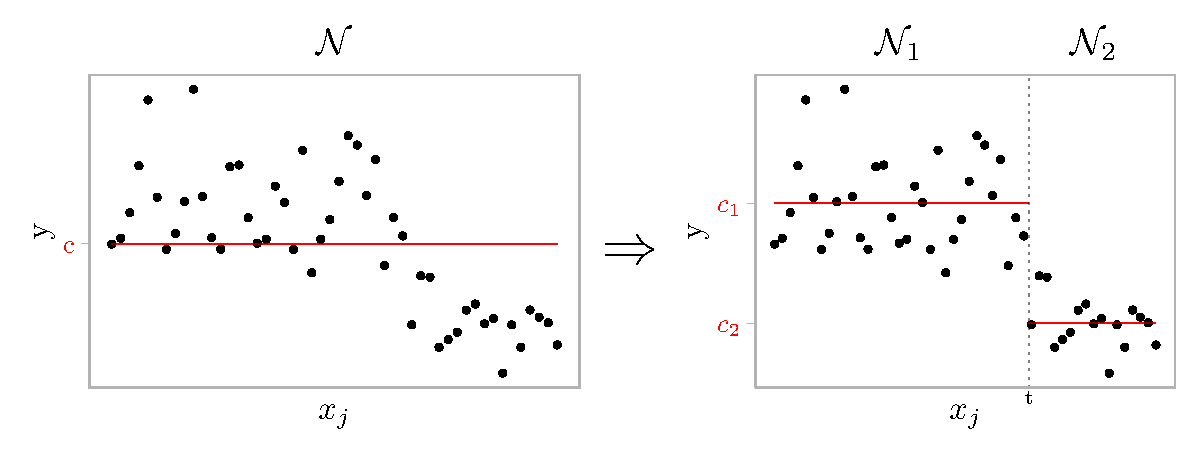
\includegraphics[width=0.975\textwidth]{../cart/figure/cart_splitcriteria_2.pdf} 
}


  \begin{itemize}
    \item Compute empirical risks in child nodes and minimize their sum to find best split (impurity reduction):
       \begin{align}
        \argmin_{j, t} \risk(N_p, j, t) &= \argmin_{j, t} \risk(N_l) + \risk(N_r) \;\;\; %\tfrac{|\Nr|}{|\Np|} 
        \end{align}
        Note: If $\risk$ is the average instead of the sum of loss functions, we need to reweight: $\tfrac{|N_{pt}|}{|N_p|} \risk(N_{pt})$
  \end{itemize}

\end{frame2}

\begin{frame2}{CART -- method summary}
  \begin{itemize}
        
    \item In general, compatible with arbitrary losses -- typical choices:
    \begin{itemize}
      \footnotesize
  
        \item $g$-way classification:
        \begin{tabular}{c |@{\vline}| c} 
   \textbf{Brier score} $\rightarrow$ \textbf{Gini} impurity & \textbf{Bernoulli} loss $\rightarrow$ \textbf{entropy} impurity \\ 
   \hline\\[-2ex]
   $\risk(N_p) = \sum\limits_{(\xv,y) \in N_p} \sum\limits_{k=1}^g
        \hat{\pik}^{(N_p)} (1 - \hat{\pik}^{(N_p)} )$ & $\risk(N_p) = -\sum\limits_{(\xv,y) \in N_p} \sum\limits_{k=1}^g
        \hat{\pik}^{(N_p)} \log \hat{\pik}^{(N_p)}$
  \end{tabular}
        
      \item Regression (\textbf{quadratic} loss): ~~
      $\risk(N_p) = \sum\limits_{(\xv,y) \in N_p} (y - c)^2$ with $c = \frac{1}{|N_p|} \sum\limits_{(\xv,y) \in N_p} y$
    \end{itemize}
  \end{itemize}
  

  
  \highlight{Optimization}
  
  \begin{itemize}
    \item \textbf{Exhaustive} search over all split candidates, choice of 
    risk-minimal split
    \item In practice: reduce number of split candidates (e.g., using quantiles instead of all observed values)
  \end{itemize}
  
  
  % \highlight{Hyperparameters} ~~ \textbf{Complexity}, i.e., 
  % number of terminal nodes $T$ (controlled indirectly, see \highlight{Implementation}) 
  

\end{frame2}


\begin{frame2}{CART -- Implementation \& Practical hints}
  \footnotesize

\highlight{Hyperparameters and complexity control}

\begin{itemize}
%\item \textbf{Complexity} control affects number of terminal nodes using different parameters
  \item Unless interrupted, splitting continues until we have pure leaf nodes (costly + overfitting)
  \item Hyperparameters: Complexity (i.e., number of terminal nodes) controlled via tree depth, minimum number of observations per node, maximum number of leaves, minimum risk reduction per split, ...
  \item Limit tree growth / complexity via
  \begin{itemize}
    \item \textbf{Early stopping:} stop growth prematurely \\ $\rightarrow$ hard 
    to determine good stopping point before actually trying all combinations
    \item \textbf{Pruning:} grow deep trees and cut back in risk-optimal manner afterwards
  \end{itemize}
\end{itemize}

\end{frame2}

\begin{frame2}{CART -- Implementation \& Practical hints}

% \highlight{Decision tree algorithms other than CART}
% %CART is a popular decision tree algorithm, 
% \begin{columns}[T, totalwidth=\linewidth]
%     \begin{column}{0.39\linewidth}
%     \vspace{-\parsep}
%         \begin{itemize}
% %\item AID (Sonquist and Morgan, 1964)
% \item CHAID (Kass, 1980)\\
% $\rightarrow$ Multi-way instead of binary splits
% \item C5.0 (Quinlan, 1993)
% \end{itemize}
%     \end{column}
%     \begin{column}{0.59\linewidth}
%     \vspace{-\parsep}
%         \begin{itemize}
% %\item Linear Model Trees (Potts, 2004)
% \item Unbiased Recursive Partitioning (Hothorn et al., 2006)\\
% $\rightarrow$ Conditional inference trees for unbiased splits
% \item Model-Based Recursive Partitioning (Hothorn et al., 2008)
% \end{itemize}
%     \end{column}
% \end{columns}
   
% \medskip

\highlight{Implementations}
\begin{itemize}
  \item \textbf{R:}
  \begin{itemize}
      \item \textbf{CART}: \texttt{mlr3} learners \texttt{LearnerClassifRpart} / 
    \texttt{LearnerRegrRpart}, calling \texttt{rpart::rpart()}
    \item \textbf{Conditional inference trees}: \texttt{partykit::ctree()} \\ mitigates overfitting by controlling tree size via p-value-based splitting
    \item \textbf{Model-based recursive partitioning}: \texttt{partykit::mob()} \\ fits a linear model within each terminal node of the decision tree
    \item \textbf{Rule-based models}: \texttt{Cubist::cubist()} for regression and \texttt{C50::C5.0()} for classification; more flexible frameworks for fitting various types of models (e.g., GLMs) within a tree's terminal nodes
  \end{itemize}
  \item \textbf{Python:} \texttt{DecisionTreeClassifier} / 
  \texttt{DecisionTreeRegressor} from package \texttt{scikit-learn}
\end{itemize}
\end{frame2}

\begin{frame2}{CART -- Pros \& Cons}
  \highlight{Dual purpose of CART} ~~ 
% As CART is a highly \textbf{unstable} learner, it is used as a base learner in bagging (random forest) or boosting ensembles to reduce the variance and improve its performance.
\begin{itemize}
    \item \textbf{Exploration purpose} to obtain interpretable decision rules (here: performance/tuning is secondary)
    \item \textbf{Prediction model}: CART as base learner in \textbf{ensembles} (bagging, random forest, boosting) can improve stability and performance (if tuned properly), but becomes less interpretable
\end{itemize}

\end{frame2}

\begin{frame2}{CART -- Pros \& Cons}
\begin{columns}[onlytextwidth]
  \begin{column}{0.5\textwidth}
    \highlight{Advantages}
    \footnotesize
    \begin{itemize}
      \positem \textbf{Easy} to understand \& visualize (\textbf{interpretable})
      \positem Built-in \textbf{feature selection}\\
      $\rightarrow$ e.g., when features are not used for splitting
      \positem Applicable to \textbf{categorical} features \\
      $\rightarrow$ e.g., $2^m$ possible binary splits for $m$ categories\\
       $\rightarrow$ trick for regr. with L2-loss and binary classif.: categories can be sorted $\Rightarrow$ $m-1$ binary splits 
      \positem Handling of \textbf{missings} possible via surrogate splits
      \positem Models  \textbf{interactions}, 
      %effects between features 
      %naturally included, 
      \positem \textbf{Fast} well scalable
      \positem High \textbf{flexibility} with custom split criteria or leaf-node 
      prediction rules
      %\positem Used in \textbf{ensembles} (bagging, random forest, boosting), improves stability and performance
    \end{itemize}
  \end{column}
  \begin{column}{0.5\textwidth}
    \highlight{Disadvantages}
    \footnotesize
    \begin{itemize}
      \negitem Rather \textbf{poor generalization} %when used stand-alone 
      \negitem High \textbf{variance/instability}: model can change a lot when training data is minimally changed
      \negitem Can \textbf{overfit} if tree is grown too deep
      \negitem Not well-suited to model \textbf{linear} relationships
      \negitem \textbf{Bias} toward features with many unique values or categories
    \end{itemize}
  \end{column}
\end{columns}
\end{frame2}

\begin{frame2}{Random Forests -- method summary}

\maketag{regression} \maketag{classification}
\maketag{NONPARAMETRIC} \maketag[50]{BLACK-BOX} \maketag{FEATURE SELECTION}


\highlight{General idea} 
\begin{itemize}
  \item \textbf{Bagging ensemble} of $M$ tree \textbf{base learners} fitted on \textbf{bootstrap} data samples\\
   ~~ $\Rightarrow$ Reduce \textbf{variance} by ensembling while slightly increasing \textbf{bias} by bootstrapping  
   \begin{itemize}
    \item Use unstable, \textbf{high-variance} base learners by letting trees grow to full size
    \item Promoting \textbf{decorrelation} by random subset of candidate features for each split
  \end{itemize}
  \item \textbf{Predict} via averaging (regression) or majority vote (classification) of base learners
\end{itemize}

\medskip

\highlight{Hypothesis space} ~~
$\Hspace = \left\{ \fx: \fx = \frac{1}{M} \sum\limits_{m = 1}^M 
\sum\limits_{t = 1}^{T^{[m]}} 
c_t^{[m]} \I(\xv \in Q_t^{[m]}) \right\}$

\end{frame2}

\begin{frame2}{Random Forests -- method summary}

  \splitVCC[0.65]{
    % FIGURE SOURCE: https://docs.google.com/presentation/d/1xodP6ayu1Gay6mMKgzVWYEFmSoeG5kNuqsaTkFFmd78  /edit
  \centering
  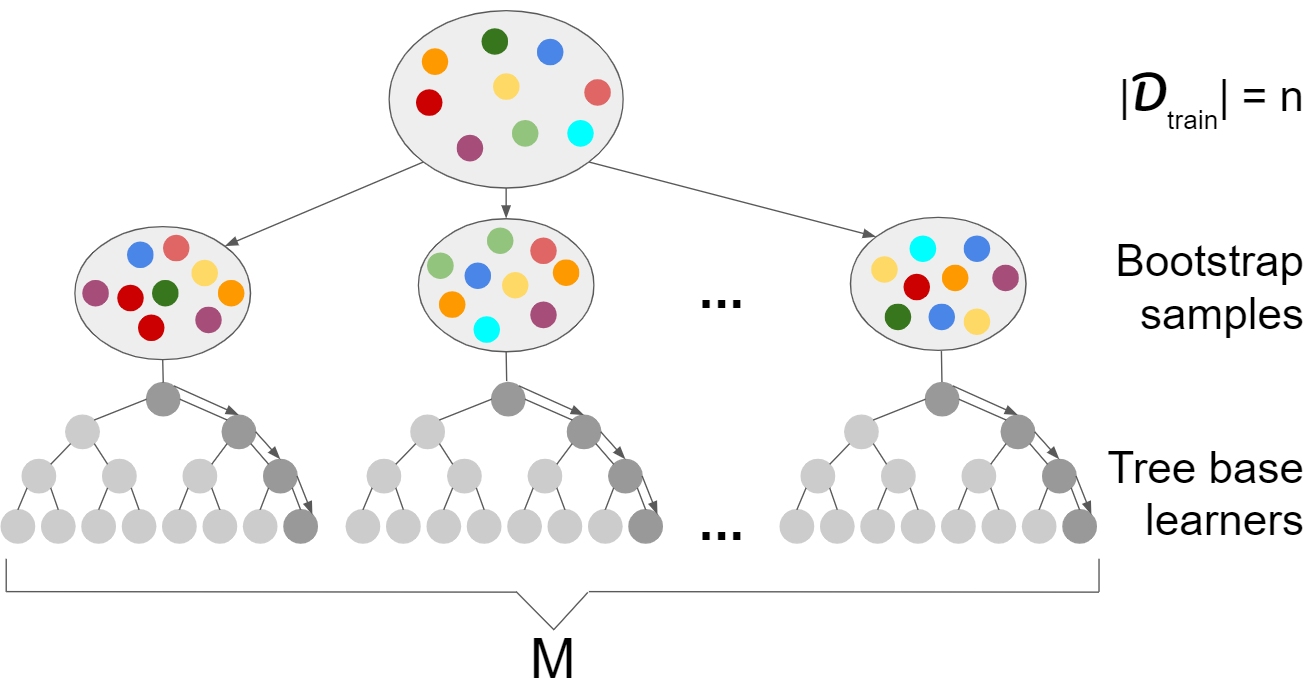
\includegraphics[width=0.6\textwidth]{figure/rf-bagging} \\
  \tiny Schematic depiction of bagging process
  }{
    \centering
  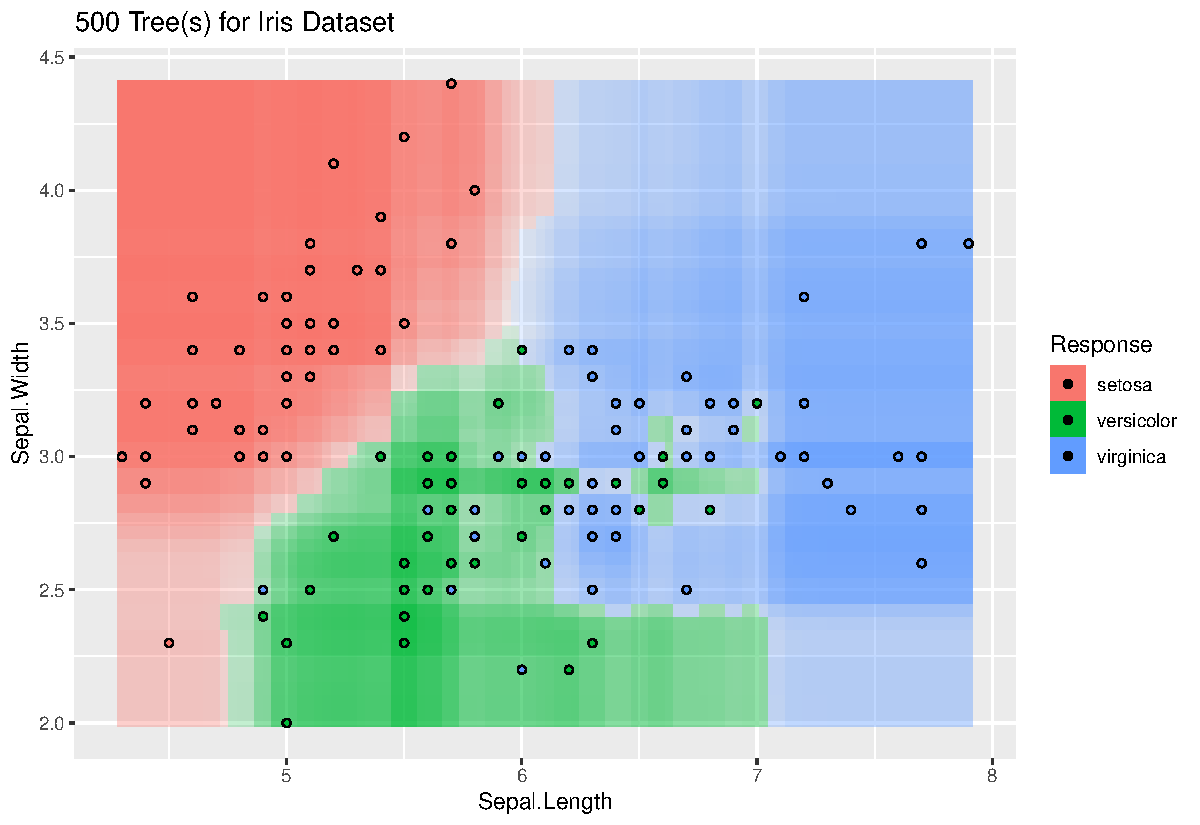
\includegraphics[width=0.9\textwidth]{
  ../forests/figure/cart_forest_intro_3} \\
  \tiny Prediction surface for \texttt{iris} data with 500-tree ensemble
  }



\highlight{Empirical risk \& Optimization} ~~ Just like tree base learners


\highlight{Out-of-bag (OOB) error}
\begin{itemize}
  \item Ensemble prediction for obs. outside individual trees' bootstrap training sample $\Rightarrow$ unseen test sample
  \item Use resulting loss as unbiased estimate of \textbf{generalization error}
  \item Mainly useful for tuning and less for model comparison as we usually compare all models uniformly by CV
\end{itemize}

\end{frame2}

\begin{frame2}{Random Forests -- method summary}

\highlight{Feature importance}

\begin{itemize}
  \item Based on \textbf{improvement in split criterion:} aggregate improvements 
  by all splits using $j$-th feature
  \item Based on \textbf{permutation:} permute $j$-th feature in 
  OOB observations and compute impact on OOB error
\end{itemize}


\highlight{Hyperparameters}

\begin{itemize}
  \item \textbf{Ensemble size}, i.e., number of trees
  \item \textbf{Complexity} of base learners, e.g., tree depth, min-split, min-leaf-size
  \item \textbf{Number of split candidates}, i.e., number of features to be considered at each split \\
  $\Rightarrow$ frequently used heuristics with total of $p$ features: 
  $\left \lfloor{\sqrt{p}}\right \rfloor$ for classification, $\left \lfloor{p/3}\right \rfloor$ for regression
\end{itemize}

% \highlight{Runtime behavior} ~~
% $\mathcal{O}(M \cdot n^2 \cdot p)$ for $M$ trees, $n$ observations and $p$ 
% features
\end{frame2}

\begin{frame2}{Random Forests -- Implementation \& Practical hints}
  \highlight{Extremely Randomized Trees}
\begin{itemize}
    \item Variance of trees can be further increased by \textbf{randomizing split points} instead of using the optimal one
    \item Alternatively consider $k$ random splits and pick the best one according to impurity 
\end{itemize}



\highlight{Tuning} 
\begin{itemize}
    \item \textbf{Ensemble size} should not be tuned as it only decreases variance $\longrightarrow$ choose sufficiently large ensemble
    \item While default values for \textbf{number of split points} is often good, tuning it can still improve performance
    \item Tuning the \textbf{minimum samples in leafs} and \textbf{minimum samples for splitting} can be benificial but no huge performance increases are to be expected 
\end{itemize}

\end{frame2}

\begin{frame2}{Random Forests -- Implementation \& Practical hints}

\highlight{Implementation}

\begin{itemize}
  \item \textbf{R:} \texttt{mlr3} learners \texttt{LearnerClassifRanger} / 
    \texttt{LearnerRegrRanger}, calling \texttt{ranger::ranger()} as a highly efficient and flexible implementation
  \item \textbf{Python:} \texttt{RandomForestClassifier} / 
  \texttt{RandomForestRegressor} from package \texttt{scikit-learn}
\end{itemize}
\end{frame2}

\begin{frame2}{Random Forests -- Pros \& Cons}

  \begin{columns}[onlytextwidth]
    \begin{column}{0.5\textwidth}
      \highlight{Advantages}
      \footnotesize
      \begin{itemize}
        \positem Retains most of \textbf{trees'} advantages (e.g., feature selection, feature interactions)
        \positem Fairly \textbf{good predictor}: mitigating base learners' variance through bagging
        \positem Quite \textbf{robust} w.r.t. small changes in data
        \positem Good with \textbf{high-dimensional} data, even in presence of noisy features
        % \positem Applicable to \textbf{unbalanced} data
        \positem Easy to \textbf{parallelize}
        \positem Robust to its hyperparameter configuration
        \positem Intuitive measures of \textbf{feature importance}
      \end{itemize}
    \end{column}
    \begin{column}{0.5\textwidth}
      \highlight{Disadvantages}
      \footnotesize
      \begin{itemize}
        \negitem Loss of individual trees' \textbf{interpretability}
        \negitem Can be suboptimal for \textbf{regression} when extrapolation is needed
        \negitem \textbf{Bias} toward selecting features with many categories (same as CART)
        \negitem Rather large model size and slow inference time for large ensembles
        \negitem Typically inferior in \textbf{performance} to tuned gradient tree boosting.
      \end{itemize}
    \end{column}
  \end{columns}
  
\end{frame2}

\begin{frame2}{Gradient Boosting -- method summary}
  % \maketag{supervised} 
\maketag{regression} \maketag{classification}
\maketag[50]{(NON)PARAMETRIC}
\maketag{BLACK-BOX}
\maketag{FEATURE SELECTION}



\highlight{General idea}

\begin{itemize}
  \item \textbf{Sequential ensemble} of $M$ \textbf{base learners} by greedy forward stagewise additive modeling
  \begin{itemize}
      \item In each iteration a base learner is fitted to current \textbf{pseudo residuals} $\Rightarrow$ one boosting iteration is one approximate \textbf{gradient step in function space}
      \item Base learners are typically \textbf{trees}, \textbf{linear regressions} or \textbf{splines}
  \end{itemize}
  \item \textbf{Predict} via (weighted) sum of base learners
  
\end{itemize}

\end{frame2}

\begin{frame2}{Gradient Boosting -- method summary}

\highlight{Hypothesis space} ~~
$\Hspace = \left\{ \fx: \fx = \sum_{m = 1}^M \beta m b(\xv, \theta m) \right\}$

\splitVCC[0.45]{
  \centering
  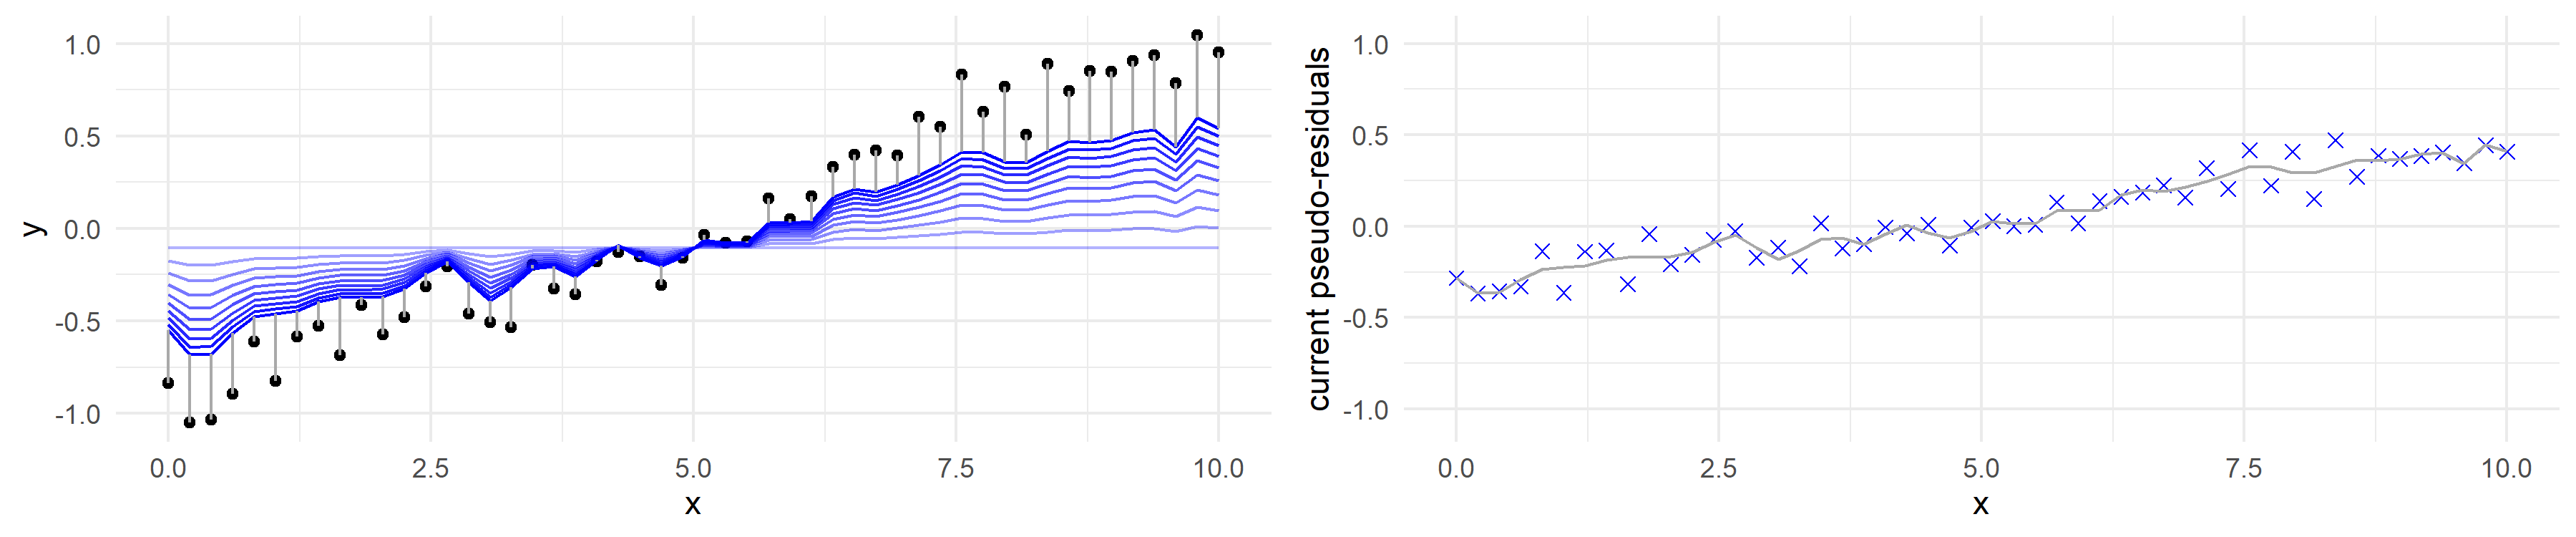
\includegraphics[width=\textwidth, trim=0 0 450 0, clip]{
  figure/illustration_gaussian_huber_2_10} \\
  \tiny{Boosting prediction function with GAM base learners for univariate 
  regression problem after 10 iterations}
}{
  % FIGURE SOURCE: http://arogozhnikov.github.io/2016/06/24/gradient_boosting_explained.html
  % 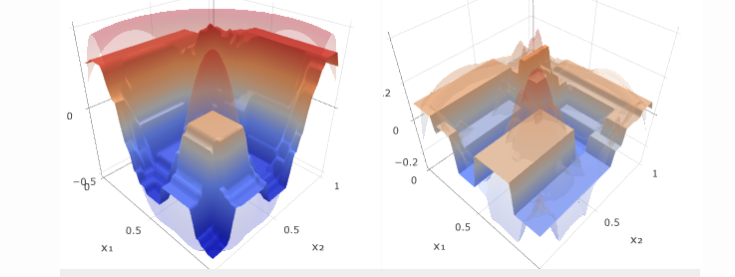
\includegraphics[width=\textwidth]{figure/gb-3d} \\
  \centering
  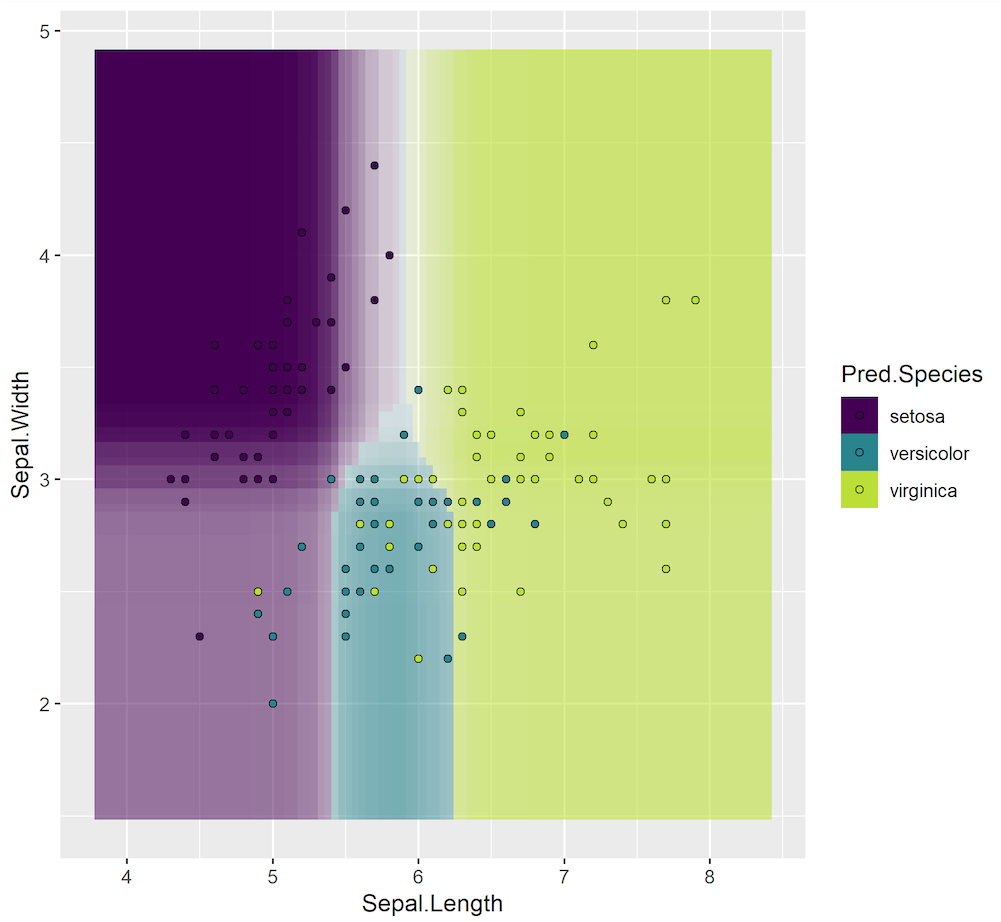
\includegraphics[width=0.5\textwidth]{
  figure/boosting_multiclass_100_single} \\
  \tiny{Boosting prediction surface with tree base learners for \texttt{iris} 
  data after 100 iterations (\textit{right:} contour lines of discriminant 
  functions)}
}

\footnotesize

\highlight{Empirical risk}

\begin{itemize}
  \item In general, compatible with any \textbf{differentiable} loss
  \item Base learner in iteration $m$ is fitted on \textbf{Pseudo residuals}: \\
  $\tilde{r}^{(i)} = - \pd{\Lxyi}{\fxi}$ by minimizing the \textbf{L2-loss}: $\sumin (\tilde{r}^{(i)} - b(\xi, \bm{\theta}))^2$
\end{itemize}

\end{frame2}

\begin{frame2}{Gradient Boosting -- method summary}


\highlight{Optimization} ~~
\begin{itemize}
    \item Same optimization procedure as base learner, while keeping the current ensemble $f m d h$ fixed\\
    $\Rightarrow$ Efficient and generally applicable since \textit{inner} loss is always L2
    \item $\beta m$ is found via \textbf{line search} or fixed to a \textbf{small constant value} and combined with the leaf values $ct m$ for tree base learners: $ct mt = \beta m \cdot ct m$
\end{itemize}


\highlight{Hyperparameters}

\begin{itemize}
  \item \textbf{Ensemble size}, i.e., number of base learners
  \item \textbf{Complexity} of base learners (depending on type used)
  \item \textbf{Learning rate} $\beta$, i.e., impact of next base learner
\end{itemize}


% \highlight{Runtime behavior} ~~ $\mathcal{O}(M \cdot n \cdot p)$ 
% for $M$ base learners, $n$ observations and $p$ features

\end{frame2}


\begin{frame2}{Gradient Boosting -- Practical hints}
  \footnotesize

\highlight{Scalable Gradient Boosting} 

\begin{itemize}
  \item \textbf{Feature and data subsampling} for each base learner fit
  \item \textbf{Parallelization} and \textbf{approximate split finding} for tree base learners
  \item GPU accelaration
\end{itemize}


\highlight{Explainable / Componentwise Gradient Boosting}
\begin{itemize}
    \item Base learners of \textbf{simple linear regression} models or \textbf{splines}, selecting a single feature in each iteration
    \item Allows \textbf{feature selection} and creates an \textbf{interpretable} model since uni- and bivariate effects can be visualized directly.
    \item Feature interactions can be learned via ranking techniques (e.g., GA$^2$M FAST)
\end{itemize}


\highlight{Tuning}
\begin{itemize}
    \item Use \textbf{early-stopping} to determine ensemble size
    \item Various \textbf{regularization parameters}, e.g., L1/L2, number of leaves, ... that need to be carefully tuned
    \item Tune learning rate and base learner complexity hyperparameters on \textbf{log-scale}
\end{itemize}

\end{frame2}

\begin{frame2}{Gradient Boosting -- Implementation}

\highlight{Gradient Tree Boosting}
\begin{itemize}
  \item \textbf{R:} \texttt{mlr3} learners \texttt{LearnerClassifXgboost} / 
  \texttt{LearnerRegrXgboost}, \texttt{LearnerClassifLightGBM} / 
  \texttt{LearnerRegrLightGBM}
  \item \textbf{Python:} \texttt{GradientBoostingClassifier} / 
  \texttt{GradientBoostingRegressor} from package \texttt{scikit-learn}, 
  \texttt{XGBClassifier} / \texttt{XGBRegressor} from package \texttt{xgboost},
  \texttt{lgb.train} from package \texttt{lightgbm}
\end{itemize}

$\Rightarrow$ \texttt{LightGBM} current state-of-the-art but slightly more complicated to use than \texttt{xgboost} 

\medskip

\highlight{Componentwise Gradient Boosting}
\begin{itemize}
    \item \textbf{R:} \texttt{mboost} from package \texttt{mboost}, 
    \texttt{boostLinear} / \texttt{boostSplines} from package \texttt{compboost}
   \item \textbf{Python:} /
\end{itemize}

$\Rightarrow$ \texttt{mboost} very flexible but slow while \texttt{compboost} is much faster with limited features

\end{frame2}

\begin{frame2}{Gradient Boosting -- Pros \& Cons}
  \footnotesize

\begin{columns}[onlytextwidth]
  \begin{column}{0.5\textwidth}
    \highlight{Advantages}
    \footnotesize
    \begin{itemize}
      \positem Retains of most of \textbf{base learners'} advantages 
      \positem Very \textbf{good predictor} due to aggressive loss minimization, typically only outperformed by heterogenous \textbf{stacking ensembles}
      \positem High \textbf{flexibility} via custom loss functions and choice of base learner
      \positem Highly efficient implementations exist (\texttt{lightgbm} / \texttt{xgboost}) that work well on large (distributed) data sets
      \positem Componentwise boosting: Good combination of (a) high performance (b) interpretable model and (c) feature selection
      % \positem Applicable to \textbf{unbalanced} data
    \end{itemize}
  \end{column}
  \begin{column}{0.5\textwidth}
    \highlight{Disadvantages}
    \footnotesize
    \begin{itemize}
      \negitem Loss of base learners' potential \textbf{interpretability}
      \negitem \textbf{Many hyperparameters} 
      to be carefully tuned
      \negitem Hard to \textbf{parallelize} ($\rightsquigarrow$ solved by efficient implementation)
    \end{itemize}
  \end{column}
\end{columns}

\end{frame2}



\begin{frame2}{Linear SVM -- method summary}
  \maketag{CLASSIFICATION} \maketag[50]{REGRESSION} \maketag{PARAMETRIC} 
\maketag{WHITE-BOX} 

\splitVCC[0.7]{
  highlight{General idea (Soft-margin SVM)}
\begin{itemize}
\item Find linear decision boundary (\textbf{separating hyperplane}) that 
\begin{itemize}
  \item maximizes distance (\textbf{margin} $\gamma$) to closest points (\textbf{support vectors, SVs}) on each side of decision boundary
  \item while minimizing margin violations (points either on \textbf{wrong side of hyperplane} or \textbf{between dashed margin line and hyperplane})
\end{itemize}

%\item \textbf{Interpretable} weighted sum of scalar product with positive coefficients for support vectors
%\item Extension to \textbf{regression} is possible but requires modifications 
%\\ $\Rightarrow$ here: only classification case
\end{itemize}
}{
  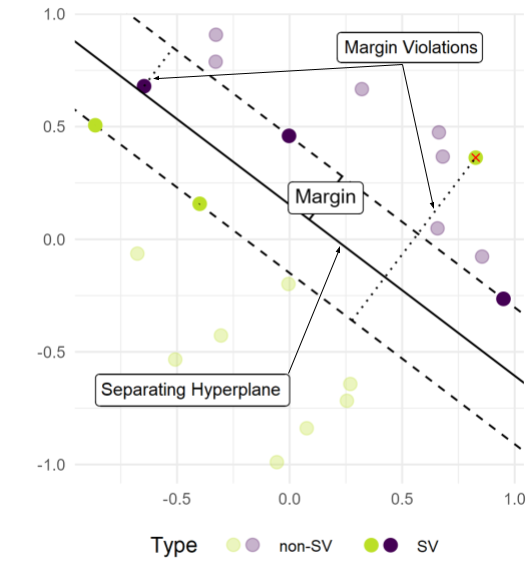
\includegraphics[width=\linewidth]{figure/svm_wording.png} \\
  \begin{center}
  \tiny{Soft-margin SVM with margin violations}
  \end{center}
}

\begin{itemize}
  \item 3 types of training points
\begin{itemize}
  \item \textbf{non-SVs} with no impact on decision boundary
  \item \textbf{SVs that are margin violators} and affect decision boundary
  \item \textbf{SVs located exactly on dashed margin lines} and affect decision boundary
\end{itemize}
\end{itemize}


\end{frame2}

\begin{frame2}{Linear SVM -- method summary}

\highlight{Hypothesis space (primal)} ~~ 
$\Hspace = \left\{\fx ~:~\fx = \thetav^\top \xv + \theta_0 \right\}$\\

\splitVCC[0.61]{

\highlight{Empirical risk} ~~ Soft-margin SVM as \textbf{L2-regularized ERM}: 
   \centerline{$\frac{1}{2} \|\thetav\|_2^2 + C \sumin \Lxyi$}
   \vspace{-\topsep}
\begin{itemize}
\setlength{\parskip}{0pt} 
\setlength{\itemsep}{0pt plus 1pt}
  \item $\|\thetav\| = 1 / \gamma$ ($\hat{=}$ maximizing margin) \\
  \item $C > 0$: penalization for margin violations
  \item Loss aims at minimizing margin violations\\
  $\rightarrow$ Classif. (\textbf{hinge} loss): $L(y,f) = \max(1-yf, 0)$ \\
  %\phantom{$\rightarrow$}$\Rightarrow$ other loss functions applicable (e.g., \textbf{Huber} loss)\\
  $\rightarrow$ Regr. (\textbf{$\eps$-insensitive} loss):   $L(y,f) = \max(|y-f| - \eps, 0)$ 
\end{itemize}
\vspace{-\topsep}

}{
  \centering
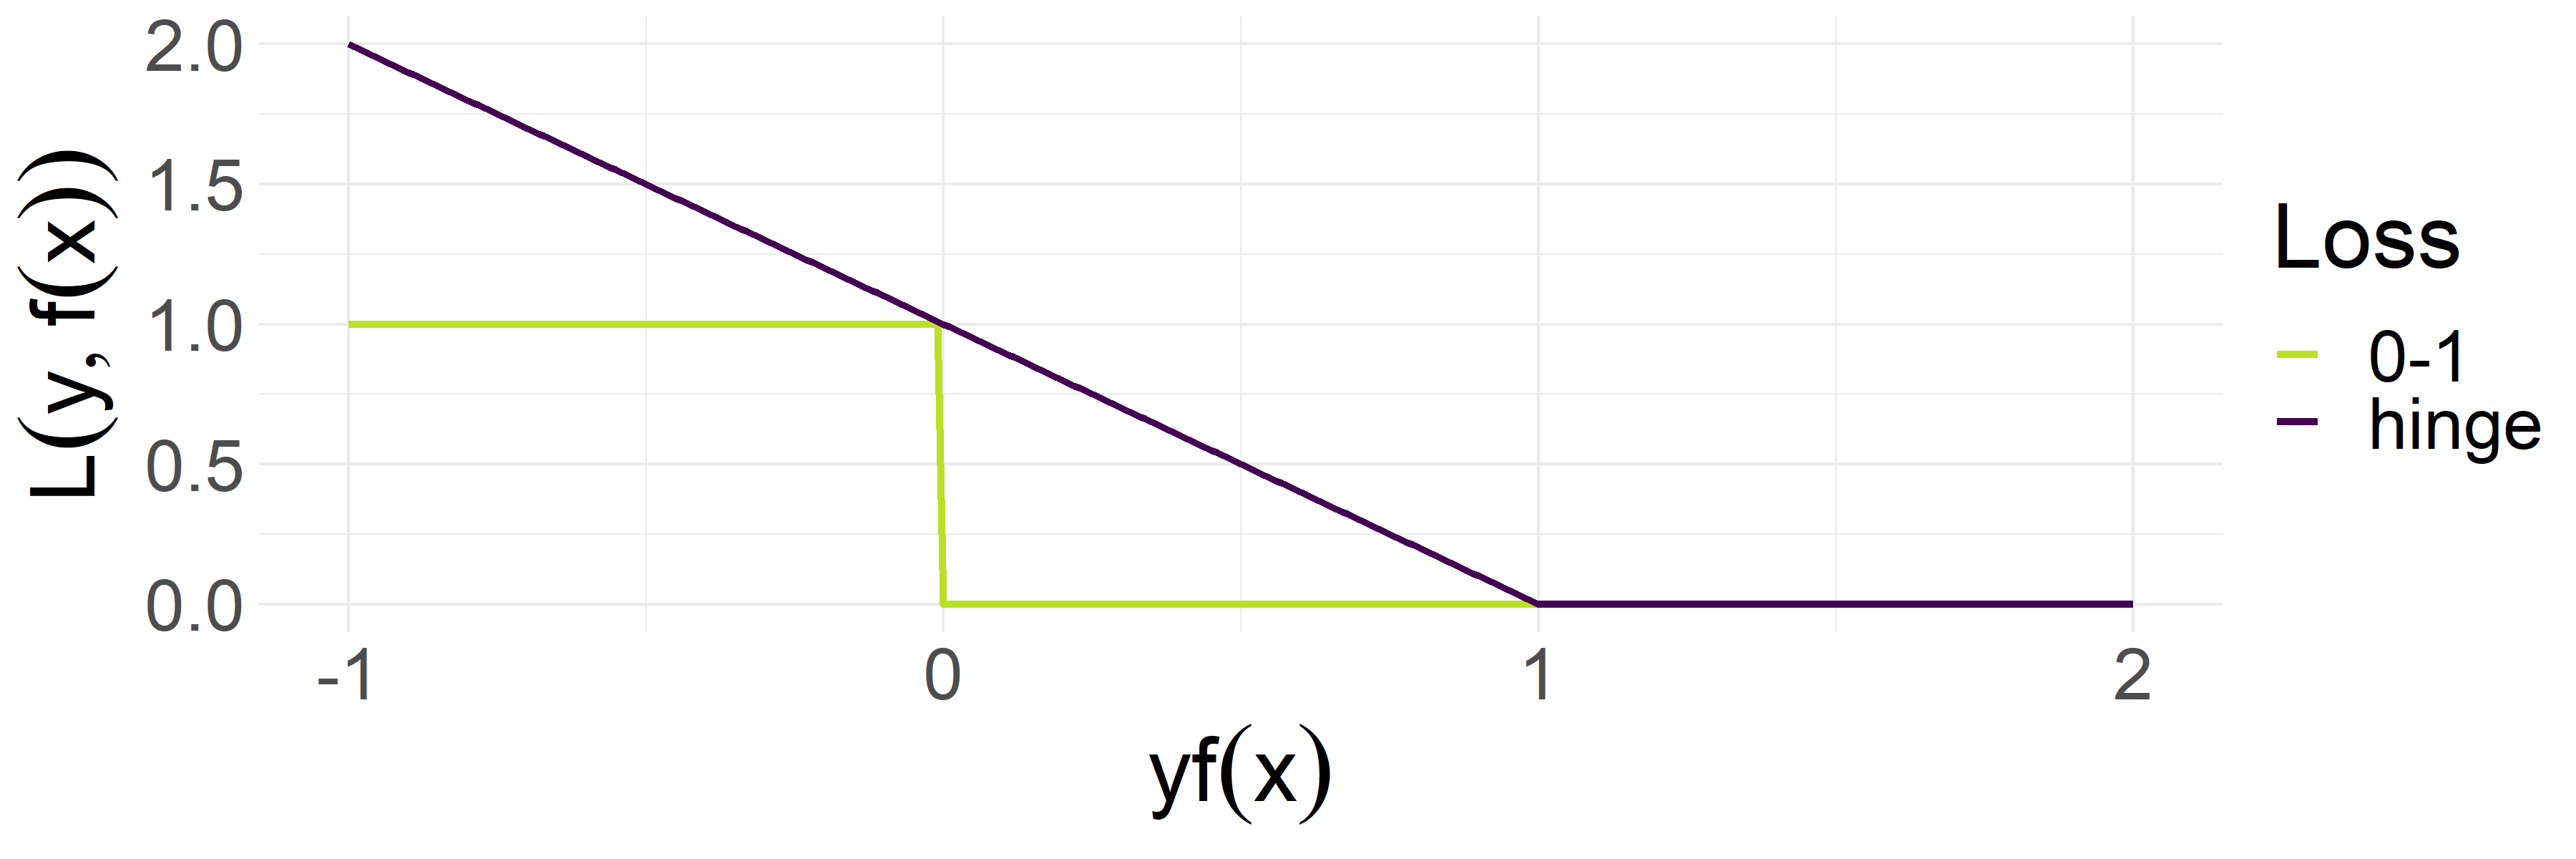
\includegraphics[height=\textwidth, keepaspectratio=true]{
figure/plot_loss_hinge.png}
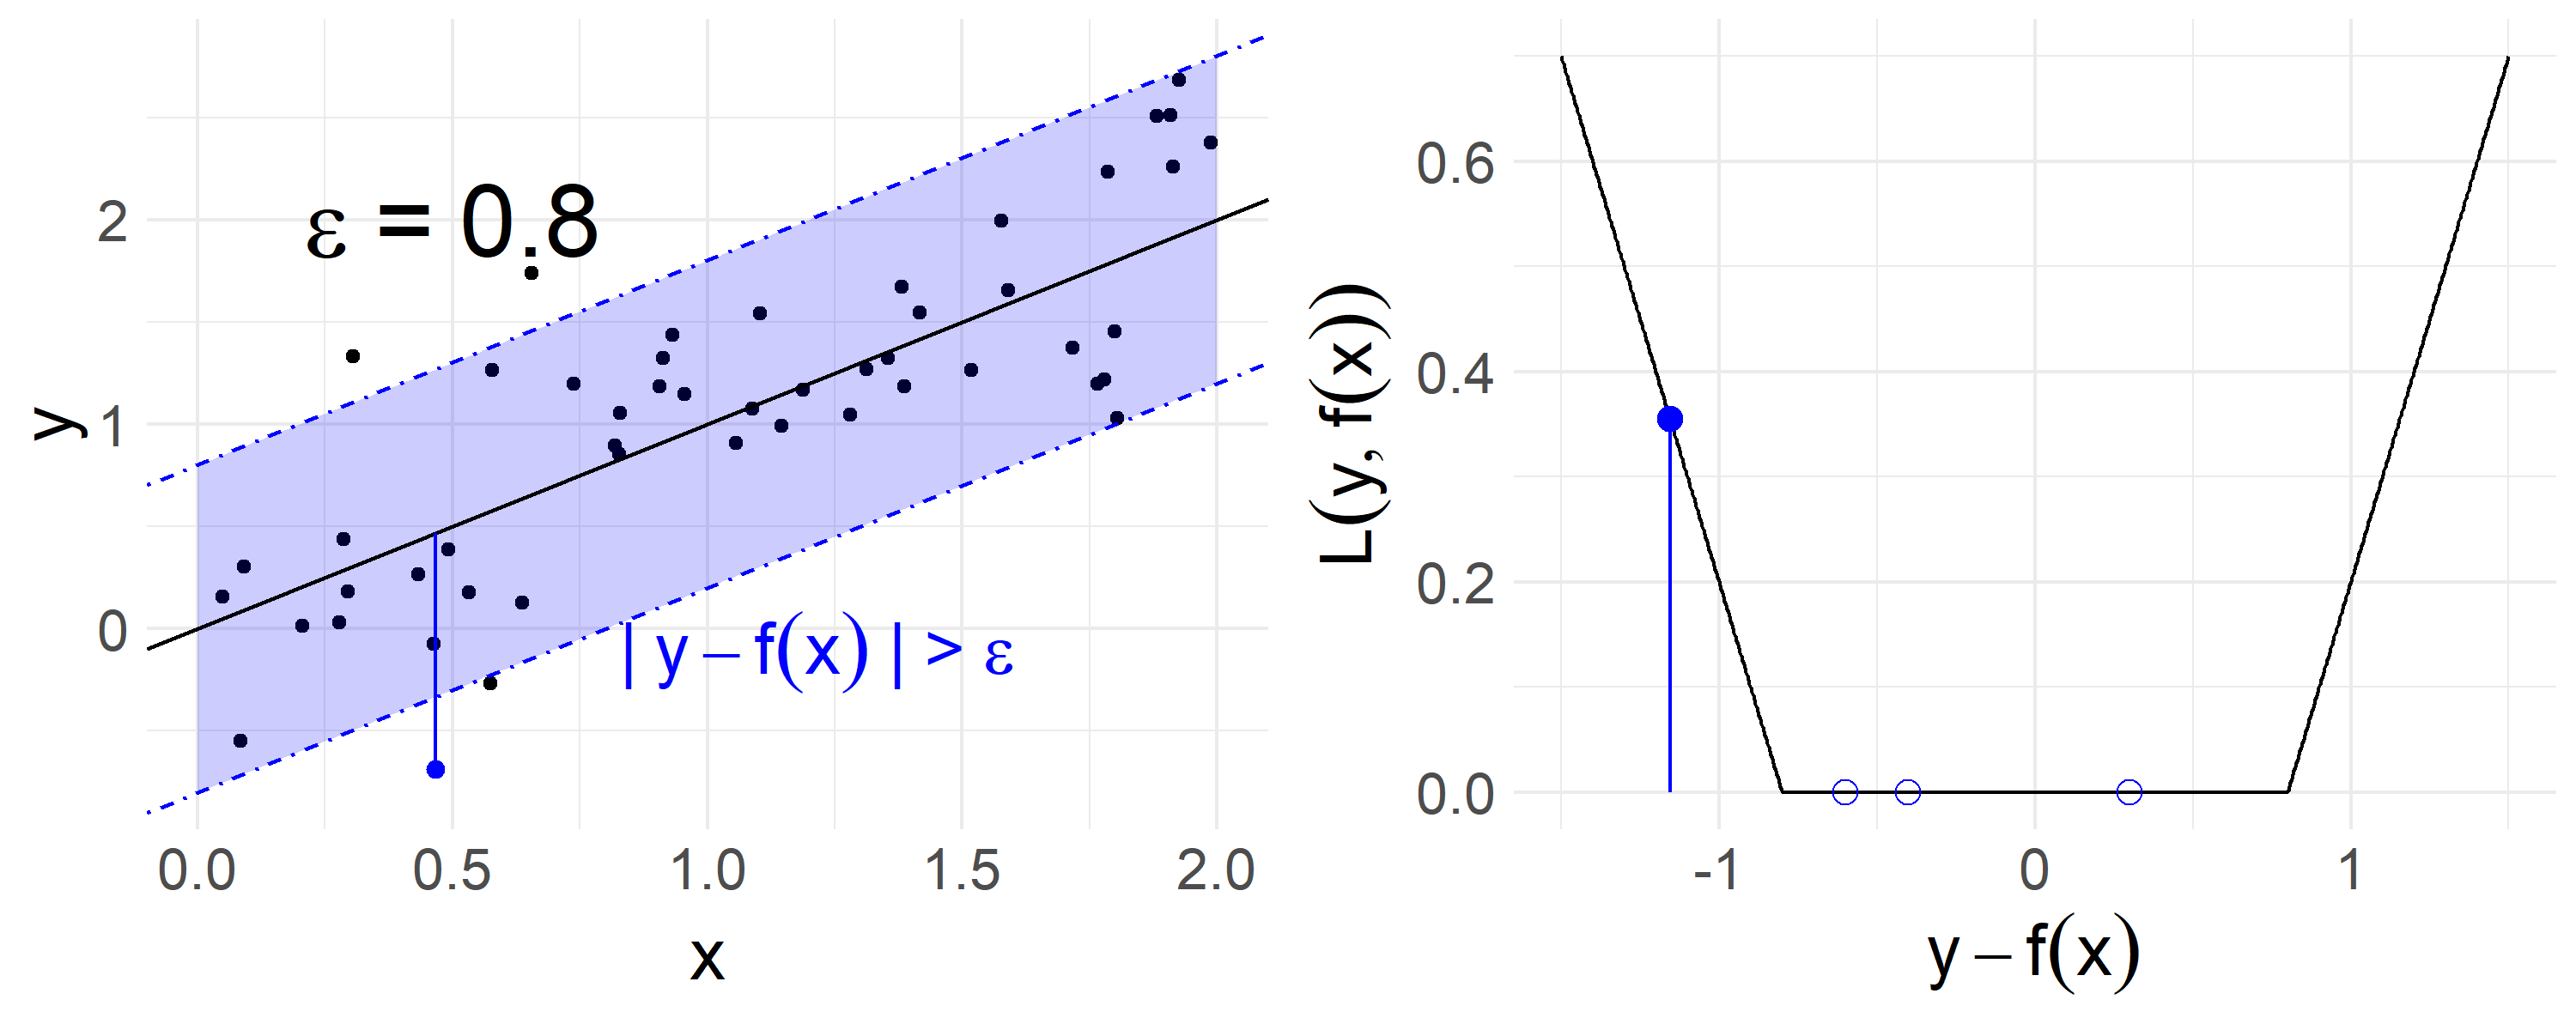
\includegraphics[height=\textwidth, keepaspectratio=true]{
figure/loss_eps_insensitive.png}
}

\end{frame2}

\begin{frame2}{Linear SVM -- method summary}

\highlight{Dual problem} ~~ %lecture_cim2\2020\08-linear-svm\slides-3-soft-margin-svm.Rnw
%\textcolor{blue}{Motivation: \dots}
SVMs as a constraint optimization (primal) problem (maximize margin s.t. constraints on obs. to limit margin violations) can be formulated as a Lagrangian dual problem with Lagrange multipliers $\alpha_i \geq 0$: % by integrating the constraints to the objective using 
$$\max\limits_{\alpha v \in \R^n} \Leftrightarrow \;\; \text{ s.t. } \;\; 0 \le \alpha_i \le C ~~ \forall i \in \nset \text{ and } \sum_{i=1}^n \alpha_i \yi = 0$$


\highlight{Solution} ~~ 
Non-SVs have $\alpha_i = 0$ as they do not affect the hyperplane

$$\fx = \sumin \alpha_i \yi \langle \xi, \xv \rangle  + \theta_0$$
%\text{ with } \alpha_i \geq 0,  \sumin \alpha_i \yi = 0 $$


\highlight{Optimization}

\begin{itemize}
\item Typically, tackling \textbf{dual} problem (though feasible 
in corresponding primal) via \textbf{quadratic programming}
\item Popular: \textbf{sequential minimal optimization} $\Rightarrow$ 
iterative algorithm based on breaking down objective into bivariate quadratic 
problems with analytical solutions
\end{itemize}

\end{frame2}

\begin{frame2}{Linear SVM -- method summary}

\highlight{Hyperparameters} ~~ Cost parameter \textbf{$C$} to control maximization of the margin vs. minimizing margin violations

\splitVCC[0.5]{
  \centering
      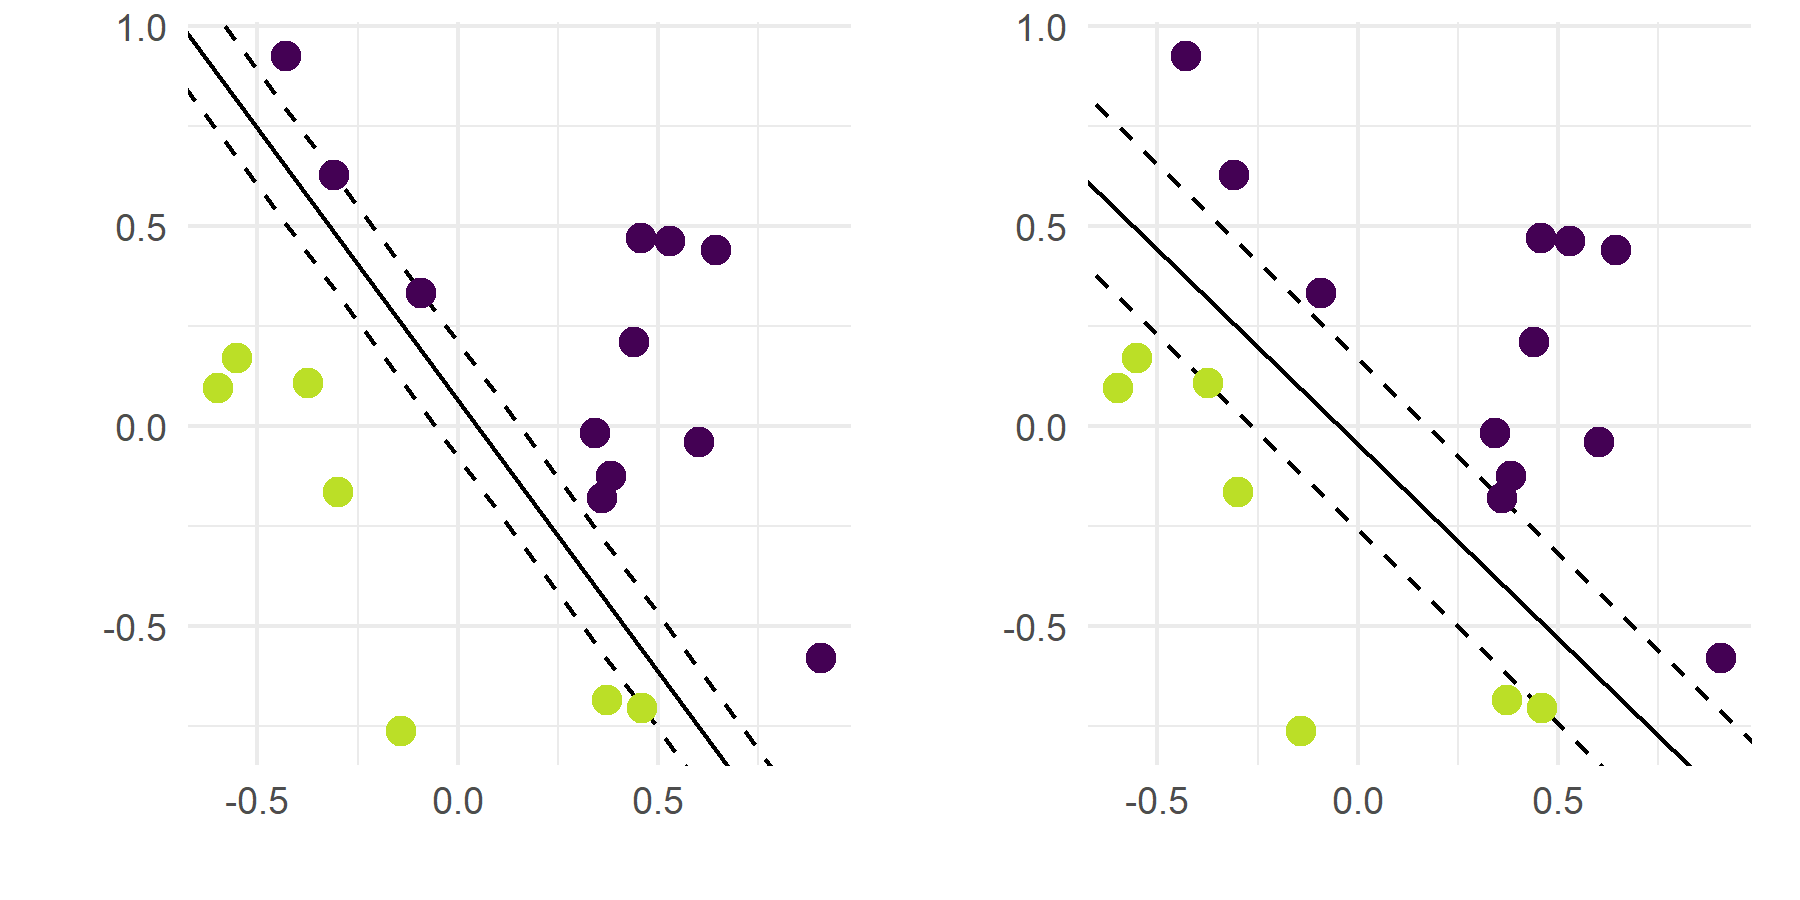
\includegraphics[width=\textwidth]{
figure/linear_classif_2.png}  \\
\tiny{Hard-margin SVM: margin is maximized by boundary on the right}
}{
  \centering
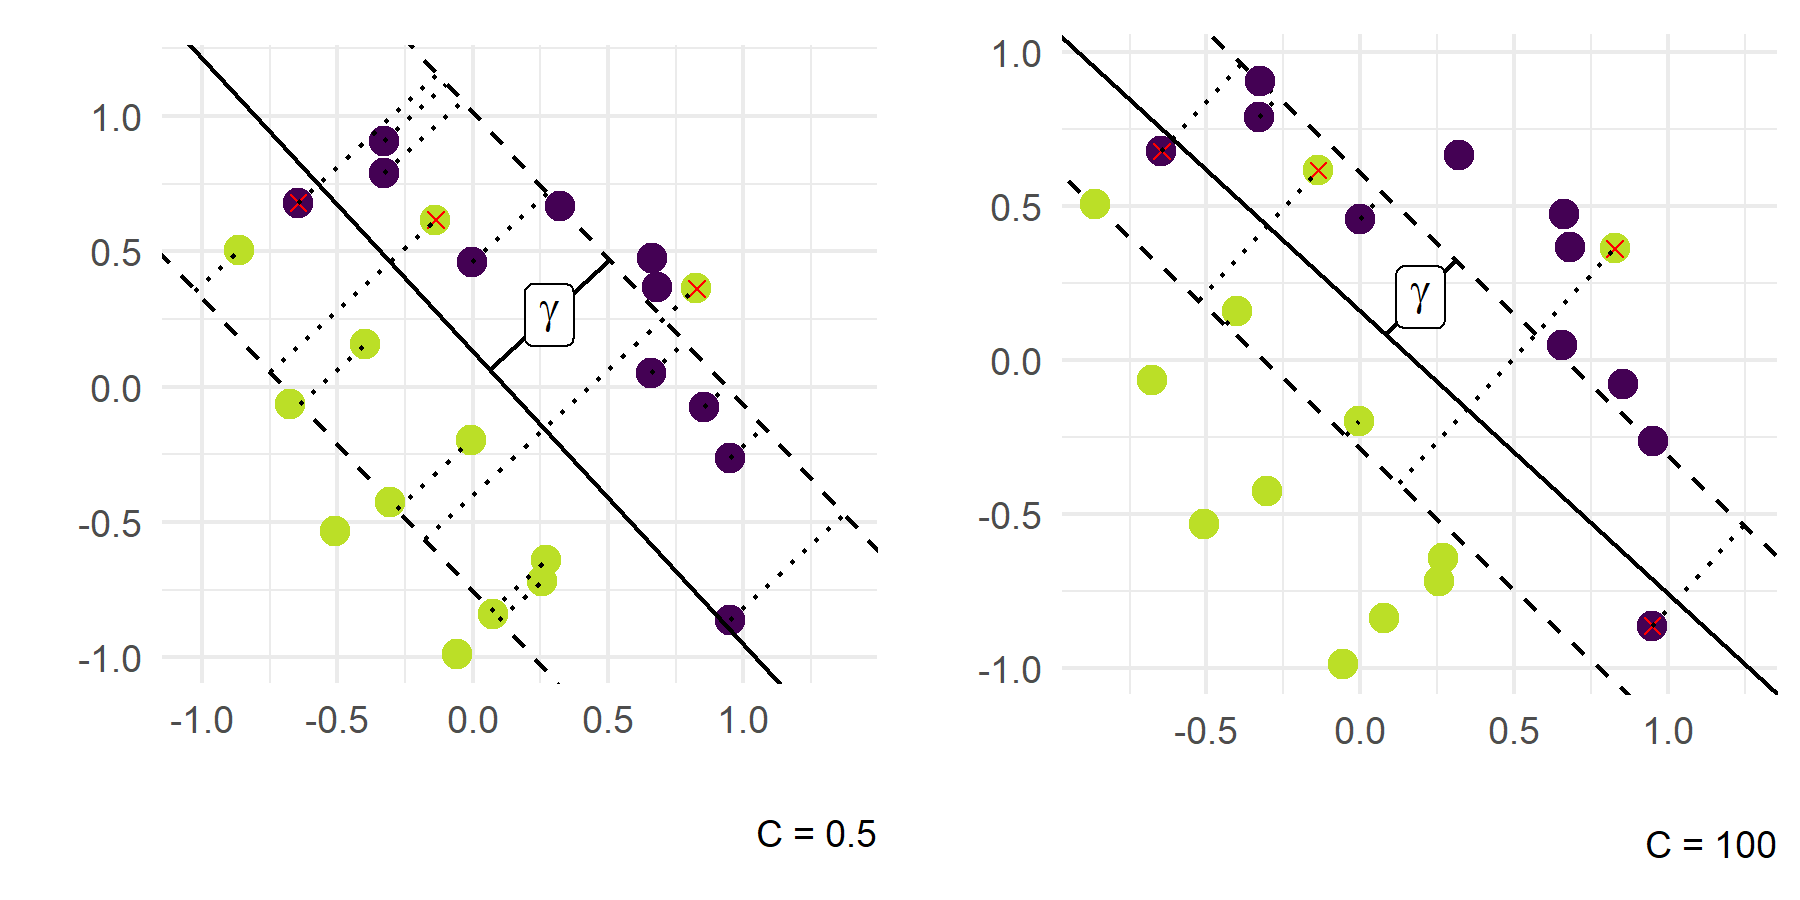
\includegraphics[width=\textwidth]{
figure/margin_violations.png}  \\
\tiny{Soft-margin SVM: large margin and few margin violations on the right (best trade-off)}
}

\normalsize

\end{frame2}

\begin{frame2}
  \footnotesize

\highlight{Preprocessing} ~~
Features should be scaled before applying SVMs (applies generally to regularized models)

\splitVCC[0.52]{
  \highlight{Tuning}

\begin{itemize}
  \item Tuning of cost parameter $C$ advisable\\
  $\Rightarrow$ strong influence 
  on resulting hyperplane
  \item $C$ it is often tuned on a log-scale grid for optimal and space-filling search space
\end{itemize}
}{
  \begin{tikzpicture}[scale=1]
    \draw [->](-0.3,0)-- (5,0) coordinate;
    \draw [->](-0.3,-1)-- (5,-1) coordinate;
    \foreach \x/\xtext/\xxtext in {0/0/1,0.5/0.5/,1/1/,1.5/1.5/,2/2/,2.5/2.5/,3/3/20,3.5/3.5/,4/4/55,4.5/4.5/90,4.60517//100} {
      \draw [very thick] (\x,-2pt) -- ++(0, 4pt) node[xshift = -6pt, yshift=-3pt,anchor=south west,baseline]{\strut$\xtext$};
      \draw [very thick] ({exp(\x)*4.5/100},-1cm+2pt) -- ++(0,-4pt) node[anchor=north]{$\xxtext$};
      \draw [->] (\x,-2pt) .. controls (\x,-1) and ({exp(\x)*4.5/100},-0.65) .. ({exp(\x)*4.5/100},-1cm);
    }
    \draw [very thick] (0,-2pt) -- ++(0, 4pt) node[xshift = -6pt, yshift=-3pt,anchor=south west,baseline]{\strut$0$};
    \draw[very thick] (4.60517,2pt) -- ++(0,-4pt) node[xshift = -1pt, yshift=3pt,anchor=north west,baseline]{\strut$log(100)$};
    \draw [very thick] (4.5/100,-1cm+2pt) -- ++(0,-4pt) node[anchor=north]{$1$};
    \draw [very thick] (4.5,-1cm+2pt) -- ++(0,-4pt) node[anchor=north]{$100$};
  \end{tikzpicture}
}

\end{frame2}

\begin{frame2}{Linear SVM -- implementation}

\highlight{Implementation} 
\begin{itemize}
  \item \textbf{R:} \texttt{mlr3} learners \texttt{LearnerClassifSVM} /
  \texttt{LearnerRegrSVM}, calling \texttt{e1071::svm()} with linear kernel (\texttt{libSVM} interface).
  Further implementations in \texttt{mlr3extralearners} based on
  \begin{itemize}
      \item \texttt{kernlab::ksvm()} allowing custom kernels
      \item \texttt{LiblineaR::LiblineaR()} for a fast implementation with linear kernel
  \end{itemize}
  \item \textbf{Python:} \texttt{sklearn.svm.SVC} from package 
  \texttt{scikit-learn} / package \texttt{libSVM}
\end{itemize}
\end{frame2}

\begin{frame2}{nonlinear SVM -- method summary}

  \footnotesize
  
  % \maketag{SUPERVISED} 
  \maketag{CLASSIFICATION} \maketag[50]{REGRESSION} \maketag{NONPARAMETRIC} 
  \maketag{BLACK-BOX}
  
  
  \highlight{General idea}
  \begin{itemize}
    \item Move \textbf{beyond linearity} by mapping data to 
    transformed space where they are linearly separable
    \item \textbf{Kernel trick} %\textcolor{blue}{(based on Mercer's theorem,  existence of reproducing kernel Hilbert space)}: 
    \begin{itemize}
      % \item Replace two-step operation feature map $\phi$ $\leadsto$ inner product 
      % by \textbf{kernel} $k: \Xspace \times \Xspace \rightarrow \R$, s.t.
      % $\scp{\phix}{\phixt} = \kxxt$
      \item No need for explicit construction of feature maps
      \item Replace inner product of feature map $\phi: \Xspace \to \Phi$ by \textbf{kernel}: $\scp{\phi x}{\phi xt} = kxxt$
    \end{itemize}
    %\item Loss of interpretability through nonlinear feature map
  \end{itemize}
  
  

  
  % \operatorname{sign}(\mathbf{w} \cdot \Phi(\mathbf{x})+b)
  
  \highlight{Hypothesis space} ~~
  % $\Hspace = \left \{ \fx = \sumin \alpha_i \yi k(\xi, \xv)  + \theta_0 ~|~
  % \theta_0, \alpha_i \in \R ~ \forall i \right \} $
  %\textcolor{blue}{$\Hspace = \{ \operatorname{sign}(\sumin \alpha_i \yi k(\xi, \xv)  + \theta_0) |\ (\theta_0, \thetav) \in \R^{p+1} \} $}
  %$\left \{ \fx = \sumin \alpha_i \yi  k(\xi, \xv)   +     \theta_0 ~|~ \alpha_i \geq 0 ~ \forall i \right \}$
  
  $\Hspace  = \left \{\fx ~:~ \fx = \sign \left( \thetav^\top \phi x + \theta_0 \right) \right \}$ (primal)
  
  $\Hspace  = \left \{\fx ~:~ \fx = \sign \left( \sumin \alpha_i \yi k(\xi, \xv) + \theta_0 \right) ~|~ \alpha_i \geq 0,  \sumin \alpha_i \yi = 0 \right \}$ (dual)%\\
  %$\Rightarrow$ \textbf{Note:} Non-SVs have $\alpha_i = 0$ as they do not affect the hyperplane
  
  % \langle \phi \left( \xi \right), \phi(\xv) \rangle

  \splitVCC[0.24]{
    centering
    \includegraphics[width=0.8\textwidth]{
    figure/circles_ds.png} \\
    \tiny{Nonlinear problem in original space} 
  }{
    \centering
    \includegraphics[width=0.9\textwidth, trim=0 30 0 50, clip]{
    figure/circles_feature_map.png} \\
    \tiny{Mapping to 3D space and subsequent linear separation -- implicitly handled by kernel in nonlinear SVM}
  }

  
  
  % \begin{minipage}[t]{0.33\textwidth}
  %   \centering
  %   \includegraphics[width=0.5\textwidth]{
  %   figure/circles_ds.png} \\
  %   \tiny{Nonlinear problem in original space} 
  % \end{minipage}
  % \begin{minipage}[t]{0.66\textwidth}
  %   \centering
  %   \includegraphics[width=0.9\textwidth, trim=0 30 0 0, clip]{
  %   figure/circles_feature_map.png} \\
  %   \tiny{Mapping to 3D space and subsequent linear separation -- implicitly 
  %   handled by kernel in nonlinear SVM}
  % \end{minipage}
  
\end{frame2}

\begin{frame2}{nonlinear SVM -- method summary}

\highlight{Dual problem} ~~ \textbf{Kernelize} dual (soft-margin) SVM problem, 
replacing all inner products by kernels:
$$\max_{\alpha v} \sumin \alpha_i - \frac{1}{2}\sumin \sumjn
\alpha_i\alpha_j\yi y^{(j)} \textcolor{blue}{k(\xi, \xi[j])}, ~~ \text{s.t. } ~~ 
0 \le \alpha_i \le C, ~~ \sumin \alpha_i \yi = 0.
$$



\highlight{Hyperparameters} ~~ Cost $C$ of margin violations, kernel 
hyperparameters (e.g., width of RBF kernel)

\end{frame2}

\begin{frame2}{nonlinear SVM -- method summary}

\splitVCC[0.59]{
  \highlight{Interpretation as basis function approach}
  \begin{itemize}
    \item \textbf{Representer theorem:} solution of dual soft-margin SVM problem is
    $\thetav = \sum_{j=1}^n \beta_j \phi (\xi[j] )$ \\
    \item Sparse, weighted sum of \textbf{basis functions}\\
    $\rightarrow \beta_j = 0$ 
    for non-SVs
    \item Result: \textbf{local} model with smoothness depending on kernel
  \end{itemize}
}{
  \centering
  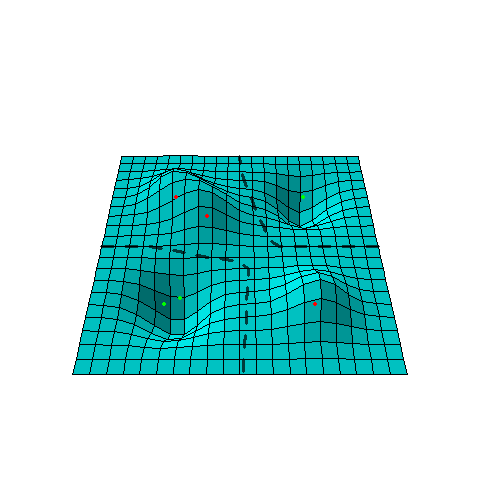
\includegraphics[width=\textwidth, trim=50 100 50 150, clip]{
  figure/svm_rbf_as_basis.png} \\
  \tiny{RBF kernel as mixture of Gaussian basis functions, forming
  bumpy, nonlinear decision surface to discern red and green points}
}



\end{frame2}


\begin{frame2}{nonlinear SVM -- Implementation \& Practical hints}

  \footnotesize
  
  \highlight{Common kernels}
  
  \begin{itemize}
    \item \textbf{Linear} kernel: dot product of given observations ~~ 
    $\Rightarrow kxxt = \xv^\top \xtil$ ~~ $\Rightarrow$ linear SVM
    \item \textbf{Polynomial} kernel of degree $d \in \N$: monomials (i.e., 
    feature interactions) up to $d$-th 
    order ~~$\Rightarrow 
    kxxt = \left(\xv^\top \xtil + b \right)^d, ~ b \geq 0$
    \item \textbf{Radial basis function (RBF)} kernel: infinite-dimensional 
    feature space, allowing for perfect separation of all finite 
    datasets ~~ $\Rightarrow kxxt = \exp \left( -\gamma \| \xv - \xtil \|_2^2 
    \right )$ with 
    bandwidth parameter $\gamma > 0$
  \end{itemize}
   

  
   \highlight{Tuning}
   
   \begin{itemize}
    \item High sensitivity w.r.t. hyperparameters, especially those of kernel
    ~~ $\Rightarrow$ \textbf{tuning} very important
    \item For RBF kernels, use \textbf{RBF sigma heuristic} to determine 
    bandwidth
  \end{itemize}
  
  
  \highlight{Implementation} 
  \begin{itemize}
    \item \textbf{R:} \texttt{mlr3} learners \texttt{LearnerClassifSVM} /
    \texttt{LearnerRegrSVM}, calling \texttt{e1071::svm()} with nonlinear kernel (\texttt{libSVM} interface),
    \texttt{kernlab::ksvm()} allowing custom kernels
    \item \textbf{Python:} \texttt{sklearn.svm.SVC} from package 
    \texttt{scikit-learn} / package \texttt{libSVM}
  \end{itemize}
  
\end{frame2}

\begin{frame2}{SVM -- Pro's \& Con's}

\begin{columns}[T, totalwidth=\textwidth]
  \begin{column}{0.5\textwidth}
    \highlight{Advantages}
    \footnotesize
    \begin{itemize}
      % \positem High \textbf{accuracy}
      \positem Often \textbf{sparse} solution (w.r.t. observations)
      \positem Robust against overfitting (\textbf{regularized}); especially in 
      high-dimensional space
      \positem \textbf{Stable} solutions (w.r.t. changes in train data)\\
      $\rightarrow$ Non-SV do not affect decision boundary
      \positem Convex optimization problem \\
      $\rightarrow$ local minimum $\hat{=}$ global minimum
      %\positem \textbf{memory efficient} (only use non-SVs)
    \end{itemize}
    
    % \highlight{Advantages (nonlinear SVM)}
    % \begin{itemize}
    %    \positem Can learn \textbf{nonlinear decision boundaries}
    %    \positem \textbf{Very flexible} due to custom kernels \\
    %    $\rightarrow$ RBF kernel yields local model \\
    %    $\rightarrow$ kernel for time series, strings etc.
    % \end{itemize}
  \end{column}

  \begin{column}{0.5\textwidth}
    \highlight{Disadvantages}
    \footnotesize
    \begin{itemize}
      \negitem \textbf{Long} training times $\rightarrow O(n^2 p + n^3)$
      %\negitem \textbf{Limited scalability} to larger data sets 
      %\textcolor{blue}{\textbf{??}}
      \negitem Confined to \textbf{linear model}
      \negitem Restricted to \textbf{continuous features}
      \negitem Optimization can also fail or get stuck
      % \negitem Poor \textbf{interpretability}
      %\negitem No handling of \textbf{missing} data
    \end{itemize}

    %     \highlight{Disadvantages (nonlinear SVM)}
    % \begin{itemize}
    %    \negitem Poor \textbf{interpretability} due to complex kernel
    %    \negitem \textbf{Not easy tunable} as it is highly important to choose the right kernel (which also introduces further hyperparameters)
    % \end{itemize}
  \end{column}
\end{columns}

\end{frame2}

\begin{frame2}{SVM -- Pro's \& Con's}



\begin{columns}[b, totalwidth=\textwidth]
  \begin{column}{0.5\textwidth}    
    \highlight{Advantages (nonlinear SVM)}
    \begin{itemize}
       \positem Can learn \textbf{nonlinear decision boundaries}
       \positem \textbf{Very flexible} due to custom kernels \\
       $\rightarrow$ RBF kernel yields local model \\
       $\rightarrow$ kernel for time series, strings etc.
    \end{itemize}
  \end{column}

  \begin{column}{0.5\textwidth}

        \highlight{Disadvantages (nonlinear SVM)}
    \begin{itemize}
       \negitem Poor \textbf{interpretability} due to complex kernel
       \negitem \textbf{Not easy tunable} as it is highly important to choose the right kernel (which also introduces further hyperparameters)
    \end{itemize}
  \end{column}
\end{columns}

% \conclbox{Very accurate solution for high-dimensional data that is linearly 
% separable}

\end{frame2}

\begin{frame2}{Neural Networks -- method summary}

  % \maketag{un/SUPERVISED} 
  \maketag{regression} \maketag{classification}
  \maketag[50]{(non)parametric}
  \maketag{BLACK-BOX} % \maketag{feature selection}
  
  \medskip
  
  \highlight{General idea}
  \begin{itemize}
    \item Learn \textbf{composite function} through series of nonlinear feature 
    transformations, represented as \textbf{neurons}, organized hierarchically 
    in \textbf{layers}
    \begin{itemize}
      \item Basic neuron operation: 1) affine \textbf{transformation} $\phi$ (weighted sum of inputs), 
      % multiplying inputs with weights (possibly including bias term), 
      2) nonlinear \textbf{activation} $\sigma$
      % , applying (nonlinear) function to transformed inputs
      \item Combinations of simple building 
      blocks to create a complex model
    \end{itemize}
    \item Optimize via \textbf{mini-batch stochastic gradient descent (SGD)} variants:
    \begin{itemize}
      \item Gradient of each weight can be infered from the \textbf{computational graph} of the network\\
      $\rightarrow$ \textbf{Automatic Differentiation} (AutoDiff)
      \item Algorithm to compute weight updates based on the loss is called \textbf{Backpropagation}
      %\textbf{Forward pass}: predict result with current parameters and 
      %compute empirical risk 
      %\item \textbf{Backward pass}: update each parameter in proportion to its 
      %error contribution $\Rightarrow$ gradients
    \end{itemize}
  \end{itemize}
  
  \medskip
   
  \highlight{Hypothesis space} ~~
  $\Hspace = \left\{ \fx: \fx = \tau \circ \phi \circ \sigma^{(h)} \circ
  \phi^{(h)} \circ \sigma^{(h - 1)} \circ \phi^{(h - 1)} \circ ... \circ 
  \sigma^{(1)} \circ \phi^{(1)} (\xv) \right\}$
  
  \smallskip
  \begin{center}
  \begin{minipage}[b]{0.24\textwidth}
    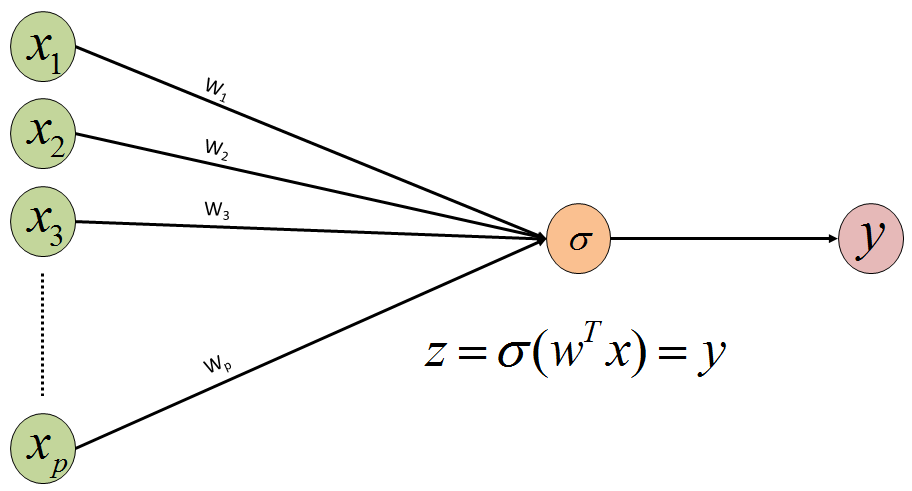
\includegraphics[width=0.9\textwidth]{figure/nn-single-neuron} \\
    %\tiny{Single neuron}
  \end{minipage}%
  \begin{minipage}[b]{0.24\textwidth}
    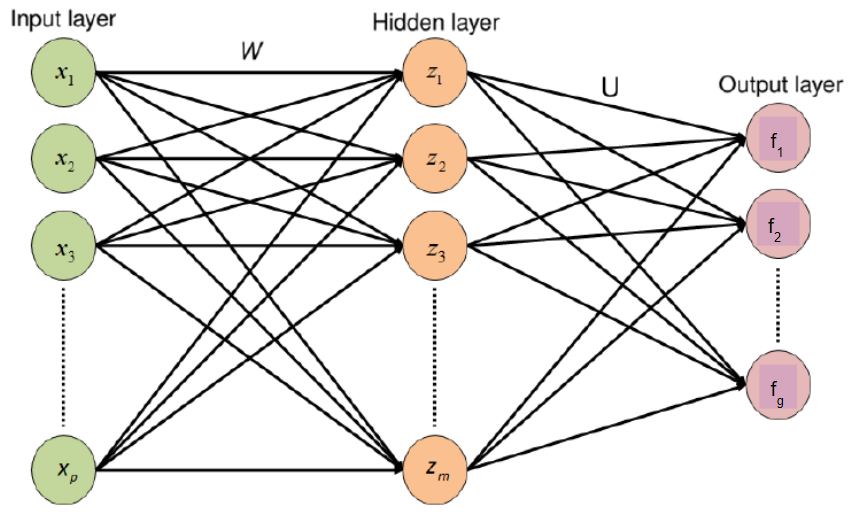
\includegraphics[width=0.9\textwidth]{figure/nn-feedforward} \\
    %\tiny{(Fully-connected) Feedforward network, 1 hidden layer}
  \end{minipage}%
  \end{center}

  \framebreak

  \footnotesize

  \highlight{Architecture}
  
  \begin{itemize}
      \item Input layer: original features $\xv$
      \item Hidden layers: nonlinear transformation of previous layer $\phi^{(h)} = \sigma^{(h - 1)}(\phi^{(h-1)})$
      \item Output layer: number of output neurons and activation depends on problem $\tau(\phi)$
      \begin{itemize}
      \item Regression: one output neuron, $\tau = $ identity
      \item Binary classification: one output neuron, $\tau = \frac{1}{1 + \exp(- \thx)}$ (logistic sigmoid)
      \item Multiclass Classification: $g$ output neurons, $\tau_j = \frac{\exp(f_j)}{\sum_{j=1}^g \exp(f_j)}$ (softmax)
  \end{itemize}
  \end{itemize}
  
  
  \highlight{Empirical risk} In general, compatible with any differentiable loss
  
  \medskip

  \framebreak
  
  \highlight{Optimization}
  
  \begin{itemize}
    \item Variety of different optimizers, mostly based on some form of 
    \textbf{stochastic gradient descent (SGD)}\\
    \item Improvements: 
      \begin{itemize}
          \item[(1)] Accumulation of previous gradients $\rightarrow$ \textbf{Momentum}
          \item[(2)] Weight specific scaling based on previous squared gradients $\rightarrow$ \textbf{RMSProb}\\
          $\Rightarrow$ \textbf{ADAM} combines (1) and (2) 
          \item[(3)] Learning rate schedules, e.g., decaying or cyclical learning rates
      \end{itemize}
      \item Training progress is measured in full passes over the full training data, called \textbf{epochs}
      \item \textbf{Batch size} is a hyperparameter and limited by input data dimension
    % \item Crucial role of \textbf{regularization} due to high expressivity of 
    % NNs' hypothesis spaces
  \end{itemize}

  \framebreak

  \highlight{Network types} ~~ Large variety of architectures for different data modelities
\begin{itemize}
  \item \textbf{Feedforward NNs / multi-layer perceptrons (MLPs):} sequence of 
  \textbf{fully-connected} layers $\Rightarrow$ tabular data
  \item \textbf{Convolutional NNs (CNNs):} sequence of feature map extractors 
  with spatial awareness $\Rightarrow$ images, time series
  \item \textbf{Recurrent NNs (RNNs):} handling of sequential, variable-length 
  information $\Rightarrow$ times series, text, audio
  \item \textbf{Transformers:} Learning invariances from data, handling multiple/any data modalities
  %\item Unsupervised: \textbf{autoencoders}, \textbf{generative adversarial networks (GANs)}, \dots
  % \item \textbf{Autoencoders:} learning unsupervised embeddings
  % \item \textbf{Generative adversarial networks (GANs):} learning to generate 
  % artificial samples
\end{itemize}

\begin{minipage}[b]{0.49\textwidth}
\begin{center}
  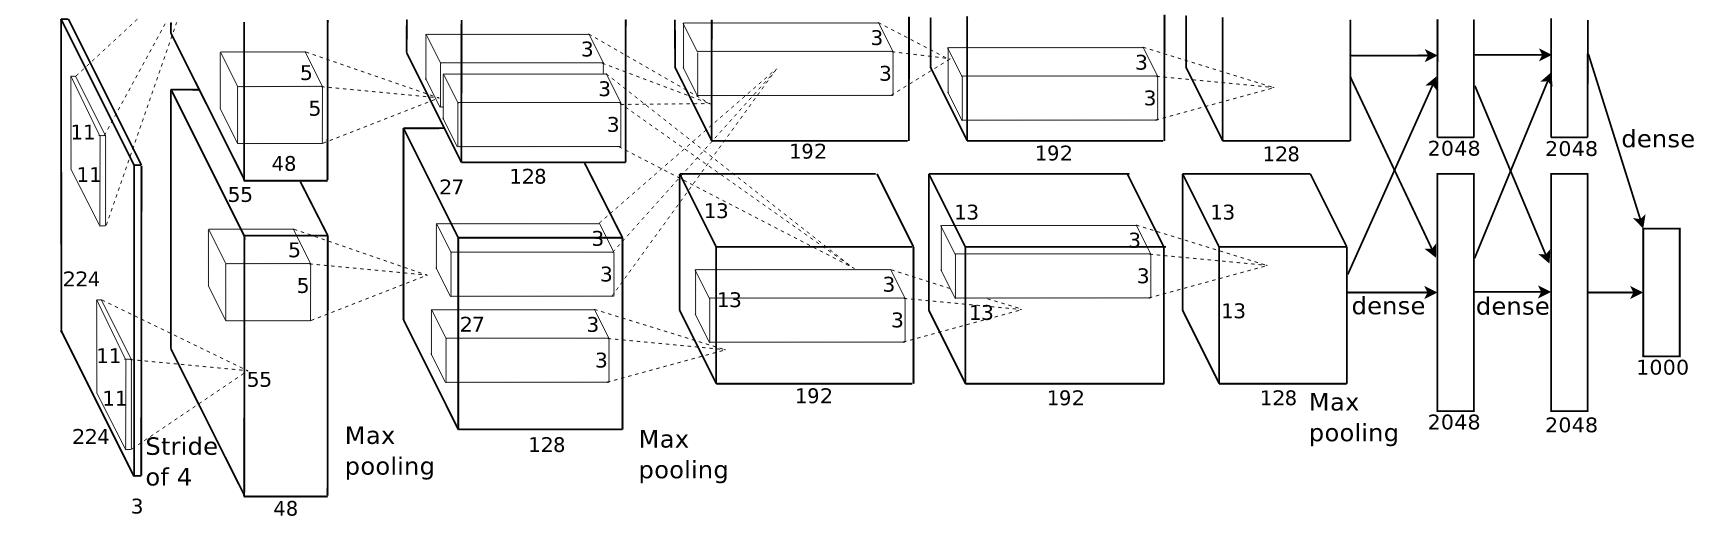
\includegraphics[width=.9\textwidth]{figure/nn-cnn-1} \\
  \tiny{Convolutional network architecture}\\ \medskip
  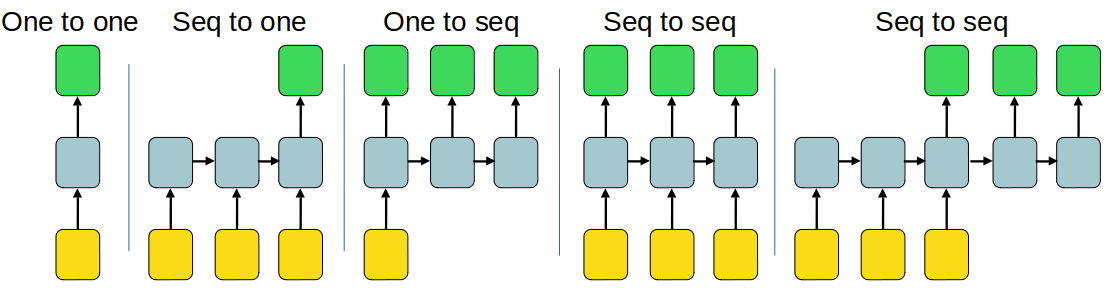
\includegraphics[width=.9\textwidth]{figure/one_to_one.png} \\
  \tiny{Recurrent network architecture}
\end{center}
\end{minipage}
\begin{minipage}[b]{0.49\textwidth}
\begin{center}
  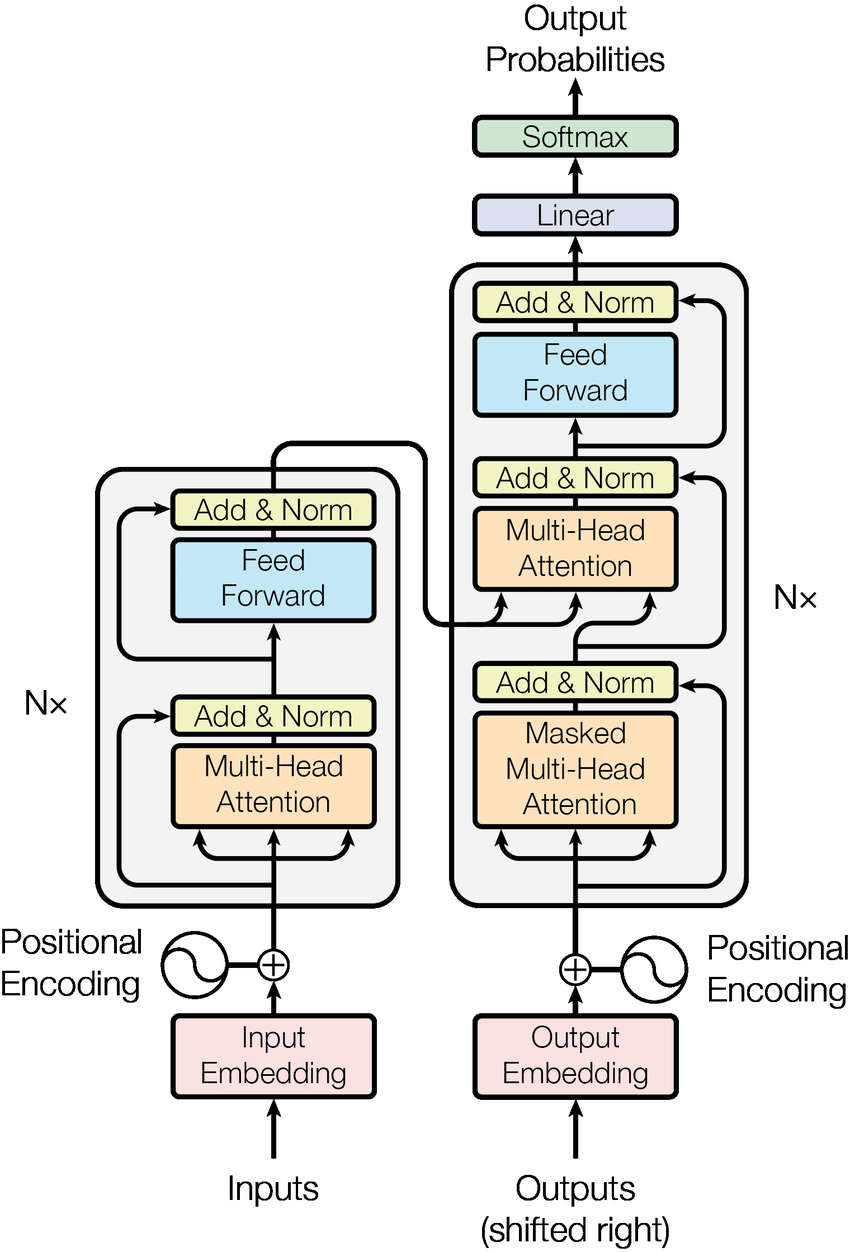
\includegraphics[width=.4\textwidth]{figure/transformer.png} \\
  \tiny{Transformer network architecture}
\end{center}
\end{minipage}

\framebreak

\footnotesize


\highlight{Hyperparameters}

\begin{itemize}
  \item \textbf{Architecture}:
  \begin{itemize}
    \item Lots of design choices $\Rightarrow$ tuning problem of its own.
    \item Typically: hierachical optimization of components (cells) and macro structure of network\\ 
    $\rightarrow$ \textbf{Neural Architecture Search (NAS)}
    \item Many predifined (well working) architectures exist for standard tasks
  \end{itemize}
  \item \textbf{Training}:
  \begin{itemize}
    \item Initial learning rate and various regularization parameters
    \item Number of epochs is determined by \textbf{early-stopping}
    \item \textbf{Data-augmentation}, e.g., applying random rotations to input images
    %Crucial due to \textbf{overparameterization} and strong 
    %\textbf{nonconvexity} 
    %\item E.g., weight initialization, choice of optimizer, learning rate, 
    %batch size, number of epochs, \dots
  \end{itemize}
\end{itemize}

\medskip

\framebreak

\highlight{Foundation models}

\begin{itemize}
    \item \textbf{Enormous} models trained on vast amounts of (general) data, e.g., all of wikipedia, in \textbf{self-supervised} fashion
    \item Used as starting point (\textbf{pre-trained}) and fine-tuned via \textbf{transfer} or \textbf{few-shot} learning for other tasks requiring little data
    \item Examples: GPT-3 for language, CLIP for vision-language, \dots
\end{itemize}

%\begin{itemize}
%    \item Makes choice of the architecture dispensable\\
%          $\Rightarrow$ Pre-defined architecture with pre-trained weights is used
%    \item Reduces training cost a lot, since pre-trained weights are only adapted during fine-tuning
%    \item \textbf{Pre-training} done in a self-supervised fashion on ubiquituous amount of data\\
%          $\Rightarrow$ In self-supervised learning, labels are generated from the data itself, no human labeling effort needed
%\end{itemize}

% \highlight{Runtime behavior} ~~ \textcolor{blue}{???}
  
\end{frame2}

\begin{frame2}
  {Neural Networks -- Implementation \& Practical hints}

\highlight{General hints}
\begin{itemize}
    \item Instead of NAS, use a standard architecture and tune training hyperparameters
    \item Training pipeline (data-augmentation, training schedules, ...) is more crucial than the specific architecture
    \item While NNets are state-of-the-art for \textbf{computer vision (CV)} and \textbf{natural language processing (NLP)}, we recommend not to use them for tabular data because alternatives perform better
    \item Computational efforts for training (and inference) can be very high, requiring specific hardware.\\
    $\rightarrow$ Using a service (esp. for foundation models) can be more cost efficient
\end{itemize}

%\highlight{Some options for regularization} 
%\begin{itemize}
%  \item Control weight magnitude with \textbf{weight decay} (L2 
%  regularization)
%  \item Interrupt training when validation error starts to pick up 
%  $\Rightarrow$ \textbf{early stopping}
%  \item Use \textbf{dropout} to deactivate neurons at random, thus down-sizing 
%  network
%  \item Expand training data and enforce invariances via \textbf{augmentation}
%  \item \dots
%\end{itemize}

%\highlight{Optimization tricks}
%\begin{itemize}
%  \item Accelerate training via optimizer (ADAM, Momentum)
%  \item Control learning rate with \textbf{schedulers}, or keep it 
%  \textbf{adaptive}
%  \item Use \textbf{batch normalization} for stability by keeping input distributions fixed throughout transformations
%  \item \dots
%\end{itemize}

% \highlight{Types of neural networks (RNNs, CNNs)}
% 
% \begin{itemize}
%   \item \textbf{Recurrent neural networks (RNNs}: Deep NN that make use of 
%   \textbf{sequential} information with temporal \textbf{dependencies} \\
%   $\rightarrow$ Frequently applied to \textbf{natural language processing}
%   \item \textbf{Convolutional neural networks (CNNs)}: Regularized version of the 
%   fully connected feed-forward NN (where each neuron is connected to all 
%   neurons of the subsequent layer) that abstracts inputs to feature maps via 
%   \textbf{convolution} \\
%   $\rightarrow$ Frequently applied to \textbf{image recognition}
% 
% \end{itemize}
% 
% \medskip
% 
% \highlight{Problem of neural architecture search (NAS)}
% 
% NN are \textbf{not off-the-shelf} methods -- the network architecture needs to 
% be tailored to each problem anew \\
% $\rightarrow$ Automated machine learning attempts to learn architectures

\medskip
 
\highlight{Implementation}

\begin{itemize}
  \item \textbf{R:} Use python libraries (below) via \texttt{reticulate}, but not really recommended except for toy applications.
  \item \textbf{Python libraries:} 
  \begin{itemize}
      \item \texttt{keras} for simple high level API 
      \item \texttt{PyTorch} for flexible design with a focus on research
      \item \texttt{TensorFlow} for flexible design with a focus on deployment / industry
      \item \texttt{huggingface} for pre-trained / foundation models
  \end{itemize}
\end{itemize}
\end{frame2}

\begin{frame2}
  {Neural Networks -- Pros \& Cons}

\footnotesize

\begin{columns}[onlytextwidth]
  \begin{column}{0.5\textwidth}
    \highlight{Advantages}
    \footnotesize
    \begin{itemize}
      \positem Applicable to \textbf{complex, nonlinear} problems
      \positem Very \textbf{versatile} w.r.t. architectures
      \positem State-of-the-art for CV and NLP
      \positem Strong \textbf{performance} if done right
      \positem Built-in \textbf{feature extraction}, obtained by intermediate
      representations
      \positem Easy handling of \textbf{high-dimensional} data
      \positem \textbf{Parallelizable} training 
    \end{itemize}
  \end{column}

  \begin{column}{0.5\textwidth}
    \highlight{Disadvantages}
    \footnotesize
    \begin{itemize}
      \negitem Typically, high computational \textbf{cost}
      \negitem High demand for \textbf{training data} 
      \negitem Strong tendency to \textbf{overfit}
      \negitem Requiring lots of \textbf{tuning expertise} 
      \negitem \textbf{Black-box} model -- hard to interpret or explain
    \end{itemize}
  \end{column}
\end{columns}
\end{frame2}


\endlecture
\end{document}






